\documentclass{sig-alternate-05-2015}
\usepackage[T1]{fontenc}
\usepackage[utf8]{inputenc}
\synctex=-1 
\usepackage[english]{babel}

\usepackage[hidelinks]{hyperref} % back-referencing + hyperlinks

\usepackage{xspace}
%\usepackage{subscript}
\usepackage{multirow}
\usepackage[font=small]{caption}
\captionsetup{skip=4pt}

\usepackage{subcaption}
\usepackage{graphicx}
\usepackage{comment}
\usepackage{tabularx}

\usepackage[normalem]{ulem}
\usepackage{fixltx2e}
\usepackage{booktabs}
\usepackage{pslatex}
%\usepackage{mathptmx,helvet,courier}
\usepackage[inline]{enumitem}
\usepackage{flushend}

\newcommand{\mytitle}{How the R Community Creates and Curates Knowledge:\\A Comparative Study of Stack Overflow and Mailing Lists}
\newcommand{\myauthor}{Carlos Arturo Gómez Teshima et al.}
\newcommand{\mysubject}{Interplay of multiple media channels}
\newcommand{\mykeywords}{Knowledge curation, Case study}

% PDF metadata. Disable when using latexdiff and enable for final version.
%\usepackage[unicode=true,
%            bookmarks=false,breaklinks=true,pdfborder={0 0 0},
%            backref=none,colorlinks=false]{hyperref}
\hypersetup{pdftitle={\mytitle},
             pdfauthor={\myauthor},
             pdfsubject={\mysubject},
             pdfkeywords={\mykeywords}
}


\newenvironment{packed_enum}{
\begin{enumerate}[itemsep=3pt, topsep=2pt, leftmargin=2.4em, parsep=0pt]
}{\end{enumerate}}

% Comments
% commands for inserting comments
\usepackage{color}
\usepackage{ifthen}
\newboolean{showcomments}
\setboolean{showcomments}{true} % toggle to show or hide comments
\ifthenelse{\boolean{showcomments}}
  {
		%\usepackage{showkeys} %Show lables and refs
		\newcommand{\nbb}[2]{
		% \fbox{\bfseries\sffamily\scriptsize#1}
		\fcolorbox{black}{yellow}{\bfseries\sffamily\scriptsize#1}
		{\sf$\blacktriangleright$\textcolor{blue}{\textit{#2}}$\blacktriangleleft$}
		% \marginpar{\fbox{\bfseries\sffamily#1}}
		}
        \newcommand{\dmg}[1]{{\color{blue}\emph{Daniel says: #1}}\xspace}
        \newcommand{\alexey}[1]{{\color{cyan}\emph{Alexey says: #1}}\xspace}
        \newcommand{\gpoo}[1]{{\color{red}\emph{Germán says: #1}}\xspace}
        \newcommand{\peggy}[1]{{\color{magenta}\emph{Peggy says: #1}}\xspace}
        \newcommand{\cassie}[1]{{\color{magenta}\emph{Cassie says: #1}}\xspace}
        \newcommand{\todo}[1]{\textcolor{red}{{\sc #1}}}
        \newcommand{\internalnote}[1]{\marginpar{\scriptsize note: #1}}
        \newcommand{\version}{\emph{\scriptsize{$-$\today$-$}}}
		\newcommand{\remarks}[1]{\color{red}[#1]\color{black}}
		\newcommand{\modified}[1]{\color{blue}[#1]\color{black}}
		\newcommand{\raw}{$\rightarrow$}
		\newcommand{\ins}[1]{\textcolor{blue}{\uline{#1}}} % please insert
		\newcommand{\del}[1]{\textcolor{red}{\sout{#1}}} % please delete
		\newcommand{\chg}[2]{\textcolor{red}{\sout{#1}}{\raw}\textcolor{blue}{\uline{#2}}} % please change
		\newcommand{\ugh}[1]{\textcolor{red}{\uwave{#1}}} % please rephrase
		\newcommand{\cn}{\textcolor{blue}{[citation needed]}\xspace}
  }
  {
        \newcommand{\dmg}[1]{}
        \newcommand{\gpoo}[1]{}
		\newcommand{\nbb}[2]{}
        \newcommand{\todo}[1]{}
        \newcommand{\internalnote}[1]{}
		\newcommand{\remarks}[1]{}
		\newcommand{\modified}[1]{#1}
		\newcommand{\version}{}
		\newcommand{\ugh}[1]{#1} % please rephrase
		\newcommand{\ins}[1]{#1} % please insert
		\newcommand{\del}[1]{} % please delete
		\newcommand{\chg}[2]{#2} % please change
		\newcommand{\cn}{}{}
  }

\newcommand{\channel}{communication channel\xspace}
\newcommand{\channels}{communication channels\xspace}
\newcommand{\Channel}{Communication channel\xspace}
\newcommand{\Channels}{Communication channels\xspace}

\newcommand{\SO}{Stack Overflow\xspace}
\newcommand{\RH}{R-help\xspace}

\newcommand{\rqa}{What types of knowledge are shared on Stack Overflow and the R-help mailing list within the R community?}
\newcommand{\rqb}{How is the knowledge constructed on Stack Overflow and the R-help mailing list?}
\newcommand{\rqc}{Why do certain users post to both Stack Overflow and the R-help mailing list?}
%\newcommand{\rqd}{What are the advantages and disadvantages of using Stack Overlow or the R-help mailing list?}

\newcommand{\reca}{Choose the correct channel}
\newcommand{\recb}{Be aware of the channel rules and the basic concepts and nomenclature used}
\newcommand{\recc}{Provide good background to the question}
\newcommand{\recd}{Learn to use external resources}
\newcommand{\rece}{Act altruistically}




%%% Local Variables:
%%% mode: latex
%%% TeX-master: "knowledge-curation.tex"
%%% End:


\begin{document}

% Copyright
\setcopyright{acmcopyright}
%\setcopyright{acmlicensed}
%\setcopyright{rightsretained}
%\setcopyright{usgov}
%\setcopyright{usgovmixed}
%\setcopyright{cagov}
%\setcopyright{cagovmixed}


% DOI
%\doi{10.475/123_4}

% ISBN
%\isbn{123-4567-24-567/08/06}

%Conference
\conferenceinfo{MSR '16}{May 14--15, 2016, Austin, TX, USA}

%\acmPrice{\$15.00}

%
% --- Author Metadata here ---
\conferenceinfo{MSR}{'16 Austin, Texas USA}
%\CopyrightYear{2007} % Allows default copyright year (20XX) to be over-ridden - IF NEED BE.
%\crdata{0-12345-67-8/90/01}  % Allows default copyright data (0-89791-88-6/97/05) to be over-ridden - IF NEED BE.
% --- End of Author Metadata ---

%
% General information
%
\title{\mytitle}

\numberofauthors{5}

\author{
\alignauthor
Carlos Gomez Teshima\\
       \affaddr{University of Victoria}\\
       \affaddr{Victoria, BC, Canada}\\
       \email{teshima@uvic.ca}
% 2nd. author
\alignauthor
Margaret-Anne Storey\\
       \affaddr{University of Victoria}\\
       \affaddr{Victoria, BC, Canada}\\
       \email{mstorey@uvic.ca}
% 3rd. author
\alignauthor 
Daniel M. German\\
       \affaddr{University of Victoria}\\
       \affaddr{Victoria, BC, Canada}\\
       \email{dmg@uvic.ca}
\and
\alignauthor
Alexey Zagalsky\\
	\affaddr{University of Victoria}\\
	\affaddr{Victoria, BC, Canada}\\
	\email{alexeyza@uvic.ca}
\alignauthor 
Lorena Casteñeda\\
       \affaddr{University of Victoria}\\
       \affaddr{Victoria, BC, Canada}\\
       \email{lcastane@uvic.ca}
}

\date{\the\year}

\maketitle

\begin{abstract}
	Media channels play an important role in the flow, construction, and curation of knowledge in software development. Understanding how developers use media channels is key to improving developer practices and supporting channel evolution. In this thesis, I investigate the way developers use media channels to curate knowledge within the R software development community. By applying a case study methodology consisting of mining archival data and survey methods, I investigate the R community on Stack Overflow and the R-help mailing list, using a qualitative approach. The findings reveal that Stack Overflow and mailing lists foster knowledge co-construction differently---crowd-sourced and participatory respectively. Furthermore, developers use actively both channels to optimize knowledge exchange and curation.

	My thesis contributes to the understanding of knowledge curation by developer communities, and describes a model for a systematic comparison of two or more media channels, within a community of practice. This model allows knowledge categorization and can be used in future studies to explore knowledge flow within multiple media channels. Moreover, based on my observations in conjunction with the survey data analysis, I extracted a set of recommendations to assist practitioners in the use of multiple Question and Answer (Q\&A) channels.
\end{abstract}

% FIXME:
%
% The code below should be generated by the tool at
% http://dl.acm.org/ccs.cfm
% Please copy and paste the code instead of the example below. 
%
 \begin{CCSXML}
<ccs2012>
<concept>
<concept_id>10011007.10011074.10011784</concept_id>
<concept_desc>Software and its engineering~Search-based software engineering</concept_desc>
<concept_significance>500</concept_significance>
</concept>
</ccs2012>
\end{CCSXML}

\ccsdesc[500]{Software and its engineering~Search-based software engineering}

%
% End generated code
%

%
%  Use this command to print the description
%
\printccsdesc

\keywords{Empirical Software Engineering; Case Study; text tagging}


\section{Introduction}
\label{cha:introduction}

	% Software development today
	Today's software development is more about just-in-time learning than reading manuals~\cite{Hartmann2008}.
	With instantaneous access to information on the Web, programmers do not have to be experts in a particular technology to build an application.
	Programmers can consult a variety of online resources (like Stack Overflow\footnote{\url{http://stackoverflow.com/}} and Nabble\footnote{\url{http://www.nabble.com/}}) by entering combinations of keywords in a search engine (e.g., Google).
	If they cannot find the correct answer there are many easy-to-use \textit{media channels} for assistance. For example, after posting a question to a specific media channel, programmers can access high-quality answers from a global user base that can easily address most programming problems within minutes or seconds~\cite{Mamykina2011}.

	% Role of media channels
	Media channels play an important role in today's knowledge economy, as well as the collaboration, coordination, and communication activities that occur between programmers. However, selecting the most appropriate media channel to transmit an idea can be challenging, given the variety of equally suitable tools and sites.
	To decide, a programmer considers which of the many channel characteristics will benefit most. Consideration might be some of the following: experts on the channel, flexibility on topics allowed, or even if the channel is asynchronous, socially enabled, or has gamification elements~\cite{Vasilescu2014c}.

	% Media channels connect communities
	Media channels are more than just delivery systems---they connect users with a \textit{community of practice} or groups of people with a common interest.
	Each community has its own implicit or explicit norms (e.g., see the R mailing list posting guide\footnote{\url{https://www.r-project.org/posting-guide.html}}).
	Any violation of the community norms or channel rules may result in unfriendly responses from the community, or being flagged with a bad reputation (e.g., Stack Overflow flags\footnote{\url{http://stackoverflow.com/help/privileges/flag-posts}}).
	Depending on the media channel, a bad online reputation can affect real life events.
	For instance, Singer \textit{et al}. found that reputation on Stack Overflow is used by recruiters to assess programmer performance~\cite{Singer2013}.

	There are multiple studies that investigate software development media channels, which provide insights on the way channels are used~\cite{Guzzi2013, Storey2014, Singer2014},  topic trends~\cite{Barua2012, Kavaler2013, Wang2013d}, best practices~\cite{Asaduzzaman2013, Treude2011, Allamanis2013}, and \textit{social programmer} behaviours~\cite{Lang2013}.
	Understanding channels is key to improve the developer practices, communication, coordination, and knowledge sharing.
	However, a review of the literature substantiates that only a few studies investigate the interplay between channels.
	Some studies that provide valuable insights on channel migration processes~\cite{Vasilescu2014c}, synergy between channels~\cite{Vasilescu2013a, Bird2006, Kavaler2013}, and channel usage~\cite{Stolee2010,Storey2014}, and yet, there is a need to analyse and compare media channels and the way programmers use them~\cite{Vasilescu2014b}.
	Questions raised that still beg unanswered are: Is one communication channel replacing the other, or are they cooperating?, Why communities have more than one channel to solve the same problem? In which circumstances one communication channel should be used over another?.

	This thesis investigated the way \textit{knowledge} (or user generated content) is curated within a particular software development community.
	For this study I chose the R community, since it provided broader relevance outside the software development community by including users with no or limited programming experience (e.g., biologist or statisticians).
	My overarching goal was to provide tools for further studies that analyse and compare the knowledge flowing through media channels.
	Thus, the R developer community has the potential for a broader selection of users' backgrounds and more diverse knowledge types. 

	By applying a qualitative \textit{exploratory case study} methodology, as proposed by Runeson \textit{et al}.~\cite{Runeson2012}, I analysed the R community on Stack Overflow\footnote{From now on, every time I refer to Stack Overflow, I are referring to the R community on Stack Overflow.} and the R-help mailing list\footnote{\url{https://stat.ethz.ch/mailman/listinfo/r-help}}, that is, the main programming related Q\&A channels that the R community contains.
	Additionally, I conducted a survey to bring further insights on the findings.
	With this findings, I constructed a series of categories that supports knowledge classification and knowledge comparison of the main type of messages (i.e., questions, answers, updates, flags and comments), which these two channels provided.
	Based on the knowledge categories analysis, I compared the way knowledge was shared on Stack Overflow and the R-help mailing list.
	Finally, I provided a set of recommendations to assist in the usage of multiple Q\&A channels, and when linking resources that are external to both channels.

\section{Research Questions}

	This thesis is based on an open challenge from Vasilescu's dissertation \textit{Social Aspects of Collaboration in Online Software Communities}~\cite{Vasilescu2014b}, that states \textit{``...to better understand the effects associated with a transition from mailing lists to social Q\&A and, e.g., whether mailing lists will eventually die off, future research could also consider analysing the content of the discussions from the two venues...''}, thus my desire is to understand the knowledge flow through channels that serve the same purpose. 

	My overarching goal was to investigate the way programmers share knowledge on Q\&A channels, the interplay of Q\&A media channels within a community, the construction of knowledge on media channels, a set of recommendation to use multiple media channels, and the way programmers use external resources in their messages.
	Therefore, the research presented in this thesis is motivated by the following research questions:

	\begin{enumerate}[\bfseries RQ-1.]
		\item What types of knowledge are shared on Stack Overflow and the R-help mailing list within the R community?

		\item How is the knowledge constructed on Stack Overflow and the R-help mailing list? 

		\item How does the sharing of links on Stack Overflow and the R-help mailing list support knowledge construction? 

		\item Why do certain users post to both Stack Overflow and the R-help mailing list?

	\end{enumerate}

\section{Contributions}

	The contributions of this thesis are summarized as follows:

	%\begin{enumerate}[\bfseries1.]
	\begin{description}
		\item[Comparison of how knowledge is shared on the two channels.]

		I compared the way knowledge is shared on both channels based on the findings of this thesis and the survey data.
		My objective was to identify the differences of how knowledge is shared on Stack Overflow and the R-help mailing list.

		\item[Categorization of messages on Q\&A media channels.]

		I built a categorization of knowledge based on the analysis of data that flows through media channels. 
		My objective was that categories should support further studies when comparing media channels based on the knowledge flowing through them.
		With these categorizations I gained insights about knowledge that flows through the channels, and the differences between them.

		\item[A set of recommendations for using multiple Q\&A media channels.]

		I created and provided a set of recommendations for using multiple media channels based on the observation and analysis of the data.
		It is meant to improve multiple media channel usage by providing a best practices reference.	

		\item[A tool to extract information from mailing lists.]

		Mailing list repositories such as R-help contain valuable information about user behaviours, best practices, topics, problems, and discussions.
		However, such information exists as unstructured data that needs special processing before it can be studied.
		To that end, I developed GTMail\footnote{This tool is available online \url{https://github.com/cagomezt/GTMail}.}, a software tool capable of dealing with multiple standardization issues when presented on mailing list data (e.g., duplicates, text formatting), extracting URLs embedded in email bodies, eliminating unnecessary information, and uploading the data to a database for further analysis.
		My tool is compatible with MBOX mailing list formats, and therefore, can be used in any other research that involves mailing list repositories.
	\end{description}

	\begin{figure}[!htb]
		\centering
		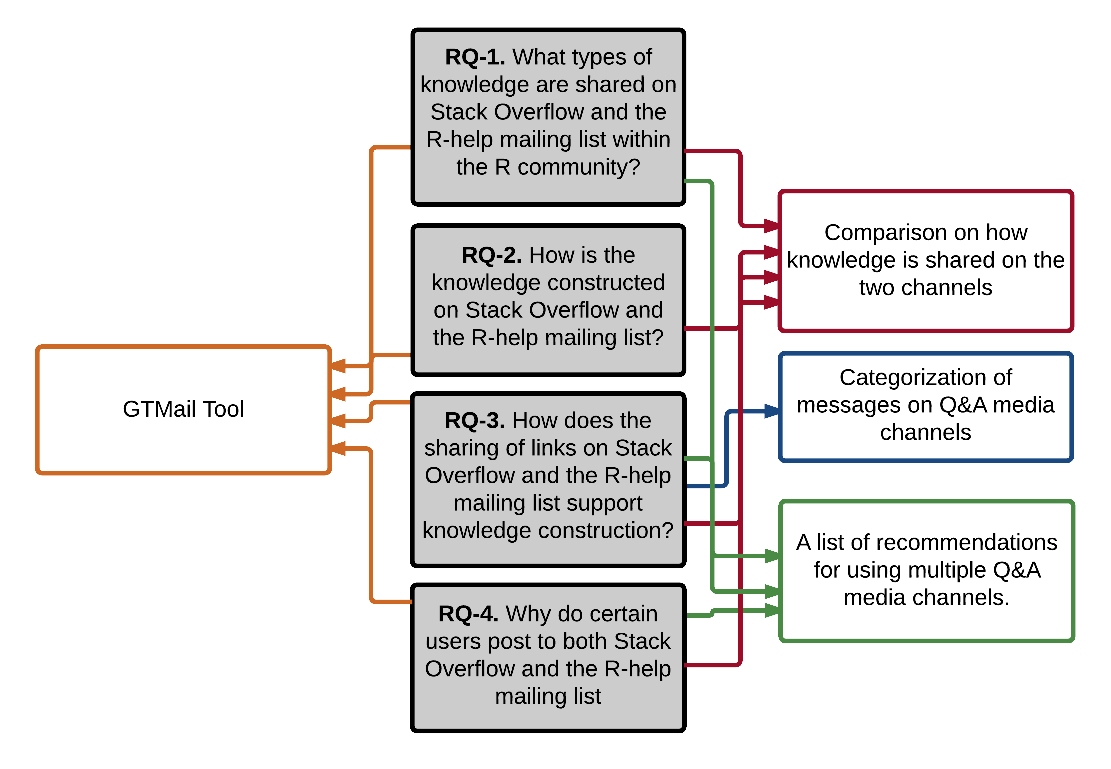
\includegraphics[width=1\columnwidth]{Figures/RQ-contributions}
		\caption{Mapping between the research questions in this thesis and the contributions.}
		\label{fig:RQ-contributions}
	\end{figure}

	Figure \ref{fig:RQ-contributions} depicts the mapping between my research questions and my contributions. 
	In the figure, GTMail tool is mapped with all research questions because the tool processes the data used in this thesis.


\section{Background}
\label{cha:background}
	% What I pretend with this part without title is to provide a non detailed introduction to all the rest of the chapter that put in context the reader. 
	% about the evolution of the channels and the ine
	Prior to the 21st century, books and classrooms were the main way to learn new programming languages and to answer questions.
	Software development was an activity performed by small geographically co-located groups using email and phone calls as the main way to coordinate activities, ask questions, collaborate with others, and share knowledge~\cite{Storey2014}.

	The emergence of new \textit{media channels} (e.g., wikis, forums, and Q\&A Websites) and \textit{communities of practice} caused a stir in the industry.  
	Project-related activities are now scattered among many channels (e.g., bug trackers, source code repositories, and project management tools)~\cite{Guzzi2013}, and learning new programming languages has become a just-in-time activity performed with the help of online resources (e.g., Stack Overflow)~\cite{Sim2013,Storey2010,Hartmann2008}.
	Many projects are now global and open to the public through online repositories (e.g., GitHub and  Bitbucket), collaboration is not limited by geographical barriers, and a new type of programmer has emerged: \textit{the social programmer}. 

	In contrast to traditional programmers, multiple sources of information make awareness one of the main issues that social programmers have to overcome on a daily basis.
	According to Storey \textit{et al}.~\cite{Storey2010, Storey2014}, the variety of channels available and personal preferences or company standards, imposes the social programmer to use multiple channels in unison.
	Regardless of how social programmers select their preferred channels, they have to invest time in learning the way each channel works.
	Also, channels are becoming increasingly complex with more options for communicating, making media literacy a complex issue.
	%information is available everywhere but the quality of it is also a concern that the social programmer have to deal with.

	These changes have attracted much of attention in the academy, and researchers have identified various aspects of media channels within communities of practice.
	For instance, we have algorithms to detect experts on social channels~\cite{Pal2011a,Pal2012a}, models that explain the propagation of information through channels~\cite{Jin2013, Jiang2013}, an understanding of the relationships between the evolution of the community and its products~\cite{German2013}, and discovered ways that social programmers are using media channels~\cite{Sowe2008a, Singh2009, Parnin2013}. 
	However, there are still many issues that current programmers need to understand, including the synergy between media channels and the way media channels are affecting communities of practices. 
	Based in my review, just a few researchers have investigated these topics. 
	Bird \textit{et al}.~\cite{Bird2006} correlated the activity in mailing lists with the activity in source code;
	Storey \textit{et al}.~\cite{Storey2014, Storey2010} identified the role of social media in software engineering;
	Kavaler \textit{et al}.~\cite{Kavaler2013} identified a complementary perspective on using APIs and the questions asked on Stack Overflow;
	and, Vasilescu \textit{et al}.~\cite{Vasilescu2013a} investigated the interplay between Stack Overflow and the software development process, which were reflected on changes committed in a source code management system (i.e., GitHub).

	The remainder of this chapter describes the background elements of this study, including the definition of media channels and communities of practice. It also introduces the R community along with the two main Q\&A media channels selected for this inquiry: the R-help mailing list and the Stack Overflow. 

\subsection{Media Channels}

	% What is a media channel?
	According to the Oxford dictionary\footnote{\url{http://www.oxforddictionaries.com/definition/english}}, a medium is \textit{``a means by which something is communicated or expressed''}. 
	Furthermore, a channel is \textit{``a method or system for communication or distribution''}.
	Taken together, a media channel is \textit{``a method or system by which information is communicated or distributed to others using different means''}.

	From the aforementioned definition, we know that a media channel is composed of users, messages, and a channel. 
	\textit{Users} are the active part of the media channel and are also responsible for the creation of messages. 
	\textit{Messages} contain the knowledge that is to be transmitted to the receiver and can take different forms depending on the channel's characteristics (e.g., text, graphics, video, sound, or a combination of characteristics).
	The \textit{channel} provides a method or system to coordinate, communicate, collaborate and share knowledge with other users~\cite{Storey2014}.

	According to Storey \textit{et al.}~\cite{Storey2014}, channel affordances are affected by their characteristics.
	Therefore, depending on the channel, some tasks are easier to accomplish than others.
	For instance, Stack Overflow is changing the way in which developers collaborate, share knowledge, learn, and communicate among themselves~\cite{Storey2014}, and may even replace the mailing list usage~\cite{Vasilescu2014b}.
	This is a consequence, according to Vasilescu \textit{et al}., of Stack Overflow's gamification system, rich interface, and social media features.

	Other authors have focused their efforts on different components and aspects of channels.
	Treude \textit{et al}. categorized questions according to their topic~\cite{Treude2011}, 
	Asaduzzaman \textit{et al}.~\cite{Asaduzzaman2013} investigated the characteristics of unanswered questions,
	and Jiang \textit{et al}. studied the way messages are disseminated on social coding sites. 
	Lastly, Vasilescu \textit{et al}. proposed a method to quantify the risk of not having maintainers for code implemented in a certain programming language~\cite{Vasilescu2013b}.

\subsection{Community of Practice}
	% What it is
	According to Wenger~\cite{Wenger2000}, a community of practice is defined as \textit{``groups of people who share a concern or a passion for something they do and learn how to do it better as they interact regularly''}. 
	In contrast with formal work groups and project teams, community members are part of the community by their own will~\cite{Wenger2000}.
	Members work towards a common objective, learning from each other, and helping each other in the process.

	% Components
	The core components of a community of practice are the domain, the practice, and the community~\cite{Wenger2011}.
	The \textit{domain}, or shared interest, defines the identity of the community.
	The \textit{practice} identifies members of a community as \textit{practitioners} that are constantly developing and sharing a set of resources (e.g., tools, documentation, histories, or experiences) to address recurring problems. 
	While the \textit{community}, comprises the activities in which members engage in discussions to help each other share information, enabling them to learn from the community.

	% Why are they important
	A community of practice is more than the sum of its parts.
	It helps members solve problems quickly, transfer best practices, develop professional skills, identify experts, form social bounds between members, and drive strategies~\cite{Wenger2011, Storey2014}.
	Communities of practice also accumulate and update knowledge through practitioners~\cite{Wenger2010}, enabling them to take a collective responsibility for managing the knowledge according to their needs~\cite{Wenger2011}.
	Wenger~\cite{Wenger2011} proposes that given the proper structure, practitioners can be the best option to manage the construction of knowledge (e.g., Stack Overflow). 

	% How they change
	Communities of practice are like living organisms, evolving and adapting according to their context, producing new tools for the community, and external sites.
	Communities change their practices and structure regularly while adapting dynamically to new situations.
	For example, Mozilla adopted the Mercurial tool~\cite{Rodriguez-Bustos2012} and changed their version release strategy~\cite{Khomh2012} as a way to keep up with a fast changing business environment.

\subsection{The R Community}

	The R project\footnote{\url{https://www.r-project.org/}} was born in 1993, as a free and open source programming language and software environment for statistical computing, bioinformatics, and graphics~\cite{Ihaka1996}. 
	R is an implementation of the S programming language combined with lexical scoping inspired by Scheme. 
	It was created by Ross Ihaka and Robert Gentleman and is now developed by the R Development Core Team.
	Today, the R community contains more than 2 million users, classified into two groups: 1.\textit{R-core} (with 20 users) consists of the software development team that maintains and evolves the R language, and 2.\textit{Periphery} includes everybody else (i.e., language users and package developers).

	I chose to study the R community because it exemplifies a typical open source community, and has been evolving for almost 20 years. 
	It provides broader relevance outside the software development community, since it includes users with no or limited programming experience (e.g., biologists or statisticians). 
	Its entire history of mailing list communication is archived and publicly available.
	Recently, the R community was also the subject of extensive research in community evolution~\cite{German2013} and the interplay between channels~\cite{Vasilescu2014c}. 

	In this thesis, I wanted to identify the interplay between media channels that serve the same purpose within a community. 
	Thus, I have focused my efforts on analysing the R-help mailing list and Stack Overflow.
	As media channels, the R-help mailing list and Stack Overflow provide similar benefits to the R community (i.e., Stack Overflow\footnote{\url{http://stackoverflow.com/tour}} and R-help\footnote{\url{https://www.r-project.org/mail.html}}).
	The R-help mailing list and Stack Overflow are one of the many channels available within the R community.
	However, I chose them because they are the channels which description are more similar in terms of the community support.

\subsubsection{R-help Mailing List}
	%\remarks{IF I HAVE TIME TALK MORE ABOUT THE OTHER CHANNELS}

	Among the communication channels that the R community uses (e.g., SVN, bug tracker system, and R Journal), there is a group of mailing lists devoted to helping community members answer questions and solve problems related to programming and the R language: the R-help, R-package-devel, R-devel, R-packages, and Bioconductor mailing lists.
	Through email, R users can send their questions to different mailing lists depending on the topic.
	Members subscribed to the R mailing lists can contribute by answering the user directly or posting to the list.
	In the last case, the email subject is kept as an identifier for the reader.

	The main objective of the R-help mailing list is to discuss problems and solutions using R. 
	However, other messages are encouraged, such as announcements (not covered by `R-announce' or `R-packages'), documentation of R, benchmarks, and examples using R. 
	It is worth noting that the R-help mailing lists are used by people who want to use R but are not necessarily knowledgeable about (or interested in) programming. 
	As a mailing list, R-help does not provide a user interface to manage the email threads.

	The R-help mailing list used to be the main media channel for asking and answering question within the R community.
	According to Vasilescu \textit{et al}.~\cite{Vasilescu2014c}, a significant number of users migrated from the R-help mailing list to Stack Overflow. 
	Despite the reduced number of users, the R-help mailing list is still a very active list; 
	on average, a subscriber can receive 55 emails a day.

\subsubsection{Stack Overflow}
\label{subsec:Rtag}

	In contrast to the R-help mailing list, Stack Overflow incorporates a rich visual and user-friendly interface with social media and gamification features.
	The social aspect of the website improves participation and provides strong support for creating and sharing knowledge as well as encouraging informal mentorship~\cite{Jenkins2009, Storey2014}.
	Meanwhile, gamification provides a system based on reputation points and badges to reward users' participation\footnote{\url{http://stackoverflow.com/help/privileges}}, thus earning points that enable functionality inside the site.
	For example, 20 points allow users to participate in the site's chat rooms, 100 points allow users to edit wiki posts, 2000 points allow users to edit questions and answers, and with 25000 points, users can access site analytics.
	Stack Overflow also provides trophies for display in users' profiles\footnote{\url{http://stackoverflow.com/help/badges}}, and a bounty reputation system to attract the interest of unanswered questions.
	According to various studies, gamification mechanisms boost participation~\cite{Vasilescu2014} and enable mutual assessment~\cite{Singer2013}.

	Stack Overflow's interface is rich with information. Figures \ref{fig:SOInterface_A} and \ref{fig:SOInterface_B} depict the interface separated into two sections. Figure \ref{fig:SOInterface_A} describes the post in relation to the \textit{question}. 
	The elements are numbered from 1 to 8, and are described as follows:
	(1) the title of the question;
	(2) the number of positive votes for the question, as well as two buttons (up and down arrows) to allow users to vote up (positive) or down (negative);
	(3) a star button to mark the question as a favourite and the number of users that have marked the question as such;
	(4) tags applied to the question;
	(5) a button to add a short, text-based comment to the question (posted below the button);
	(6) the body of the question which might contain, along with the description, other aids such as images, source code, examples, and links;
	(7) the last user that edited the question along with their reputation points;.
	and (8) information about the user who posted the question, including their alias, silver and copper badges, and the date of the posted question.

	\begin{figure}[!htb]
	\centering
	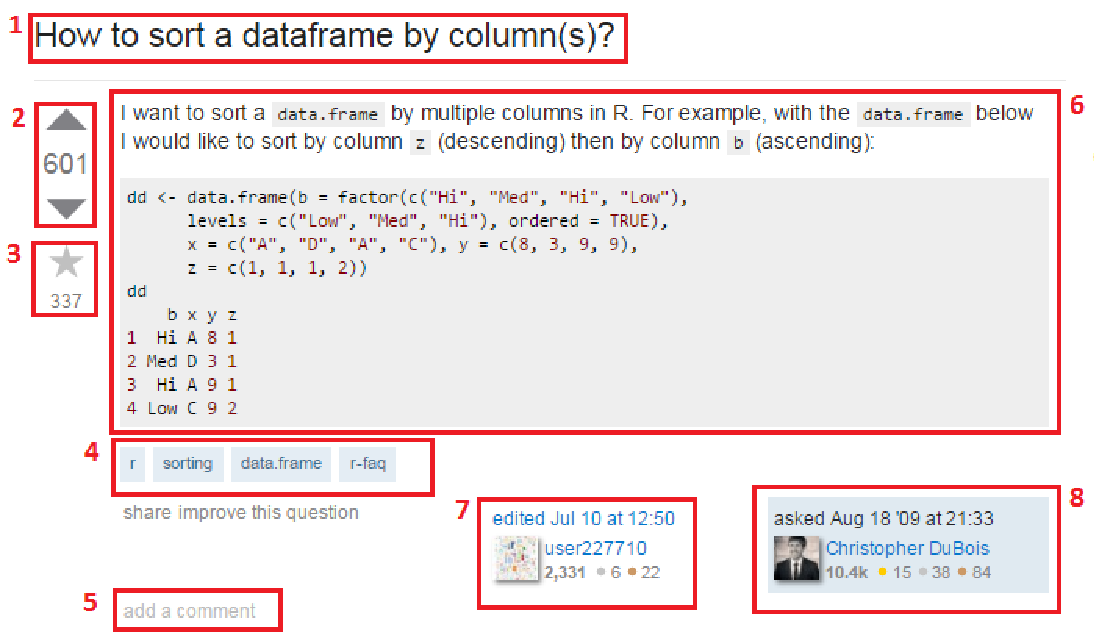
\includegraphics[width=0.8\columnwidth]{Figures/SOInterface_A}
	\caption{Stack Overflow interface [Question section]}
	\label{fig:SOInterface_A}
	\end{figure}

	Figure \ref{fig:SOInterface_B} shows the post in relation to the \textit{answer} located below the question in the interface.
	The elements are numbered 1 to 8, and are described as follows:
	(1) the number of answers provided to the question;
	(2) sorting buttons that allow users to display the answers by latest activity, oldest first, or most recent first;
	(3) the number of positive votes for the answer, as well as two buttons (up and down arrows) to allow users to vote up (positive) or down (negative);
	(4) a check mark to indicate that the owner of the question marked the answer as the solution to the question;
	(5) the body of the answer which might contain, along with the proposed solution, other aids such as images, source code, examples, and links;
	(6)	the last user that edited the question along with their reputation points;
	(7) information about the user who posted the question, including their alias, silver and copper badges, and the date of the posted question;
	and (8) the comments to the answer, which are fairly short and limited to include only text.

	\begin{figure}[!htb]
	\centering
	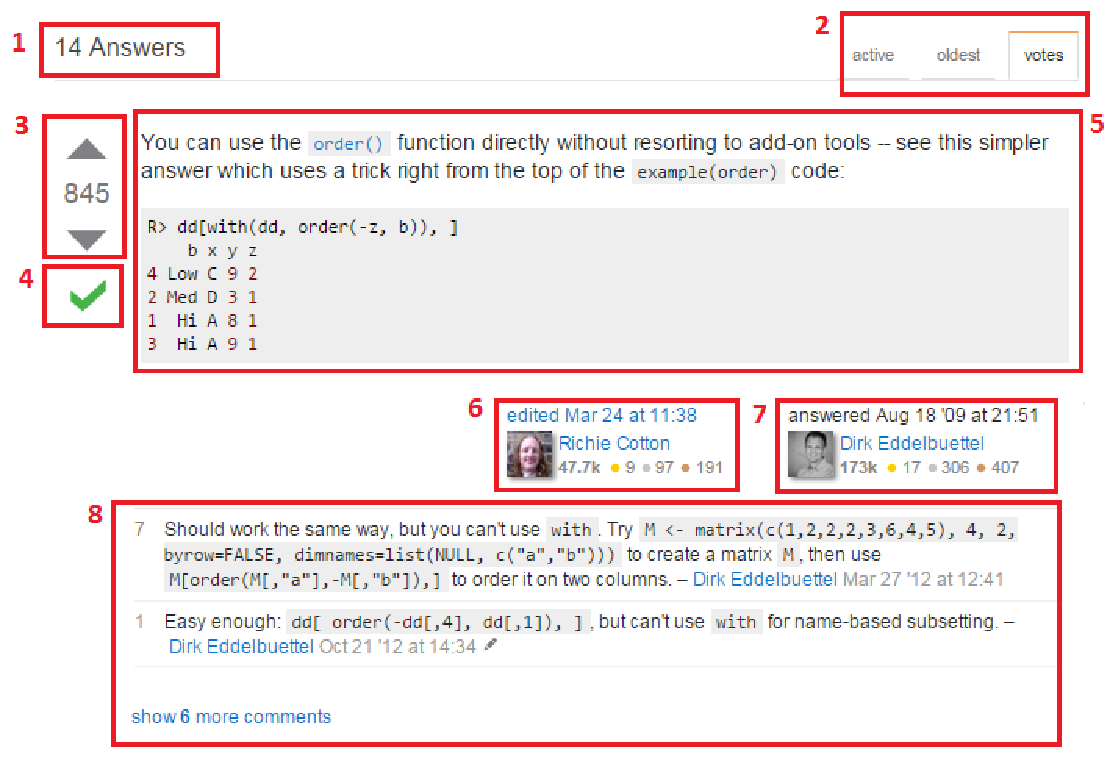
\includegraphics[width=0.8\columnwidth]{Figures/SOInterface_B}
	\caption{Stack Overflow interface [Answer Section]}
	\label{fig:SOInterface_B}
	\end{figure}

	The adoption of social media has occurred at a much faster rate than any previous communication technology \cite{Chui2012}.
	In the last decade, Stack Overflow has become the most popular media channel for answering software development related questions, nearly replacing previous methods of communication that accomplished the same objective (e.g., mailing list)~\cite{Vasilescu2014c}.
	%<<
	Figure \ref{fig:VasilescuFA1} shows the number of questions asked each month on Stack Overflow, Cross Validate and the R-help mailing list (TOP), and the number of questions answered on the R-help mailing list (after September 2008) and Stack Exchange each month (BOTTOM).
	%>>
	Despite Stack Overflow's advantages over Q\&A mailing lists such as the R-help (i.e., social network features, gamification environment and rich visual user interface), there are still many users who prefer the latter.
	Later in this thesis, we learn about the way programmers use Stack Overflow and the R-help mailing list to gain and share knowledge.

	\begin{figure}
		\centering
		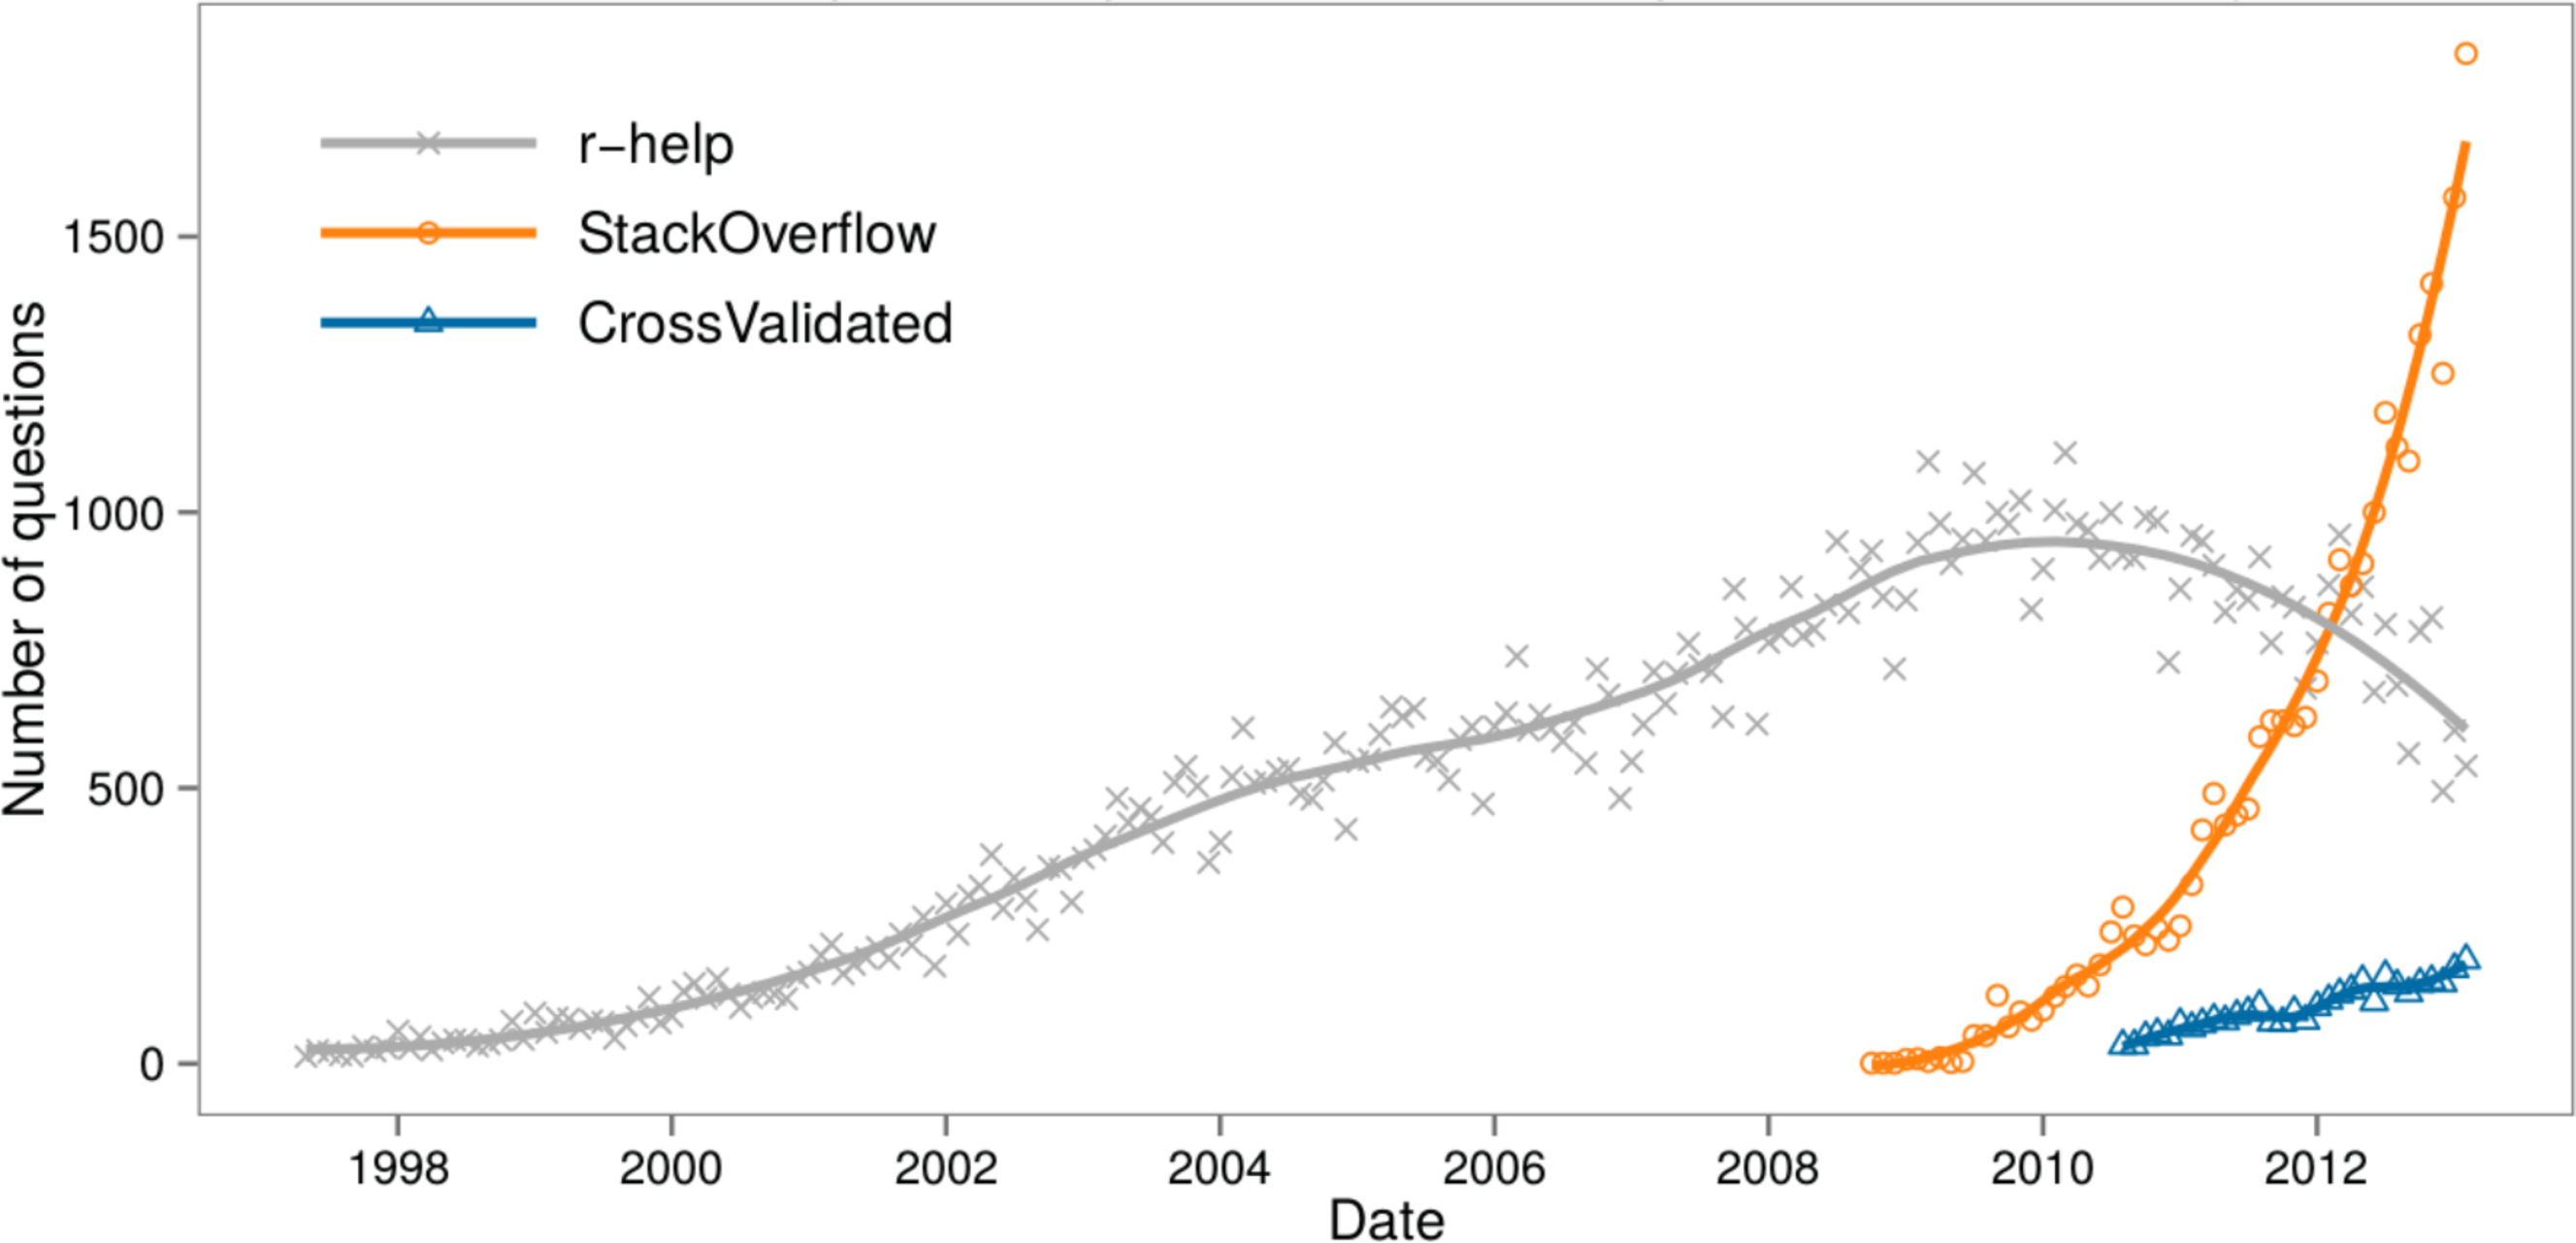
\includegraphics[width=1\columnwidth]{Figures/VasilescuFA1}
		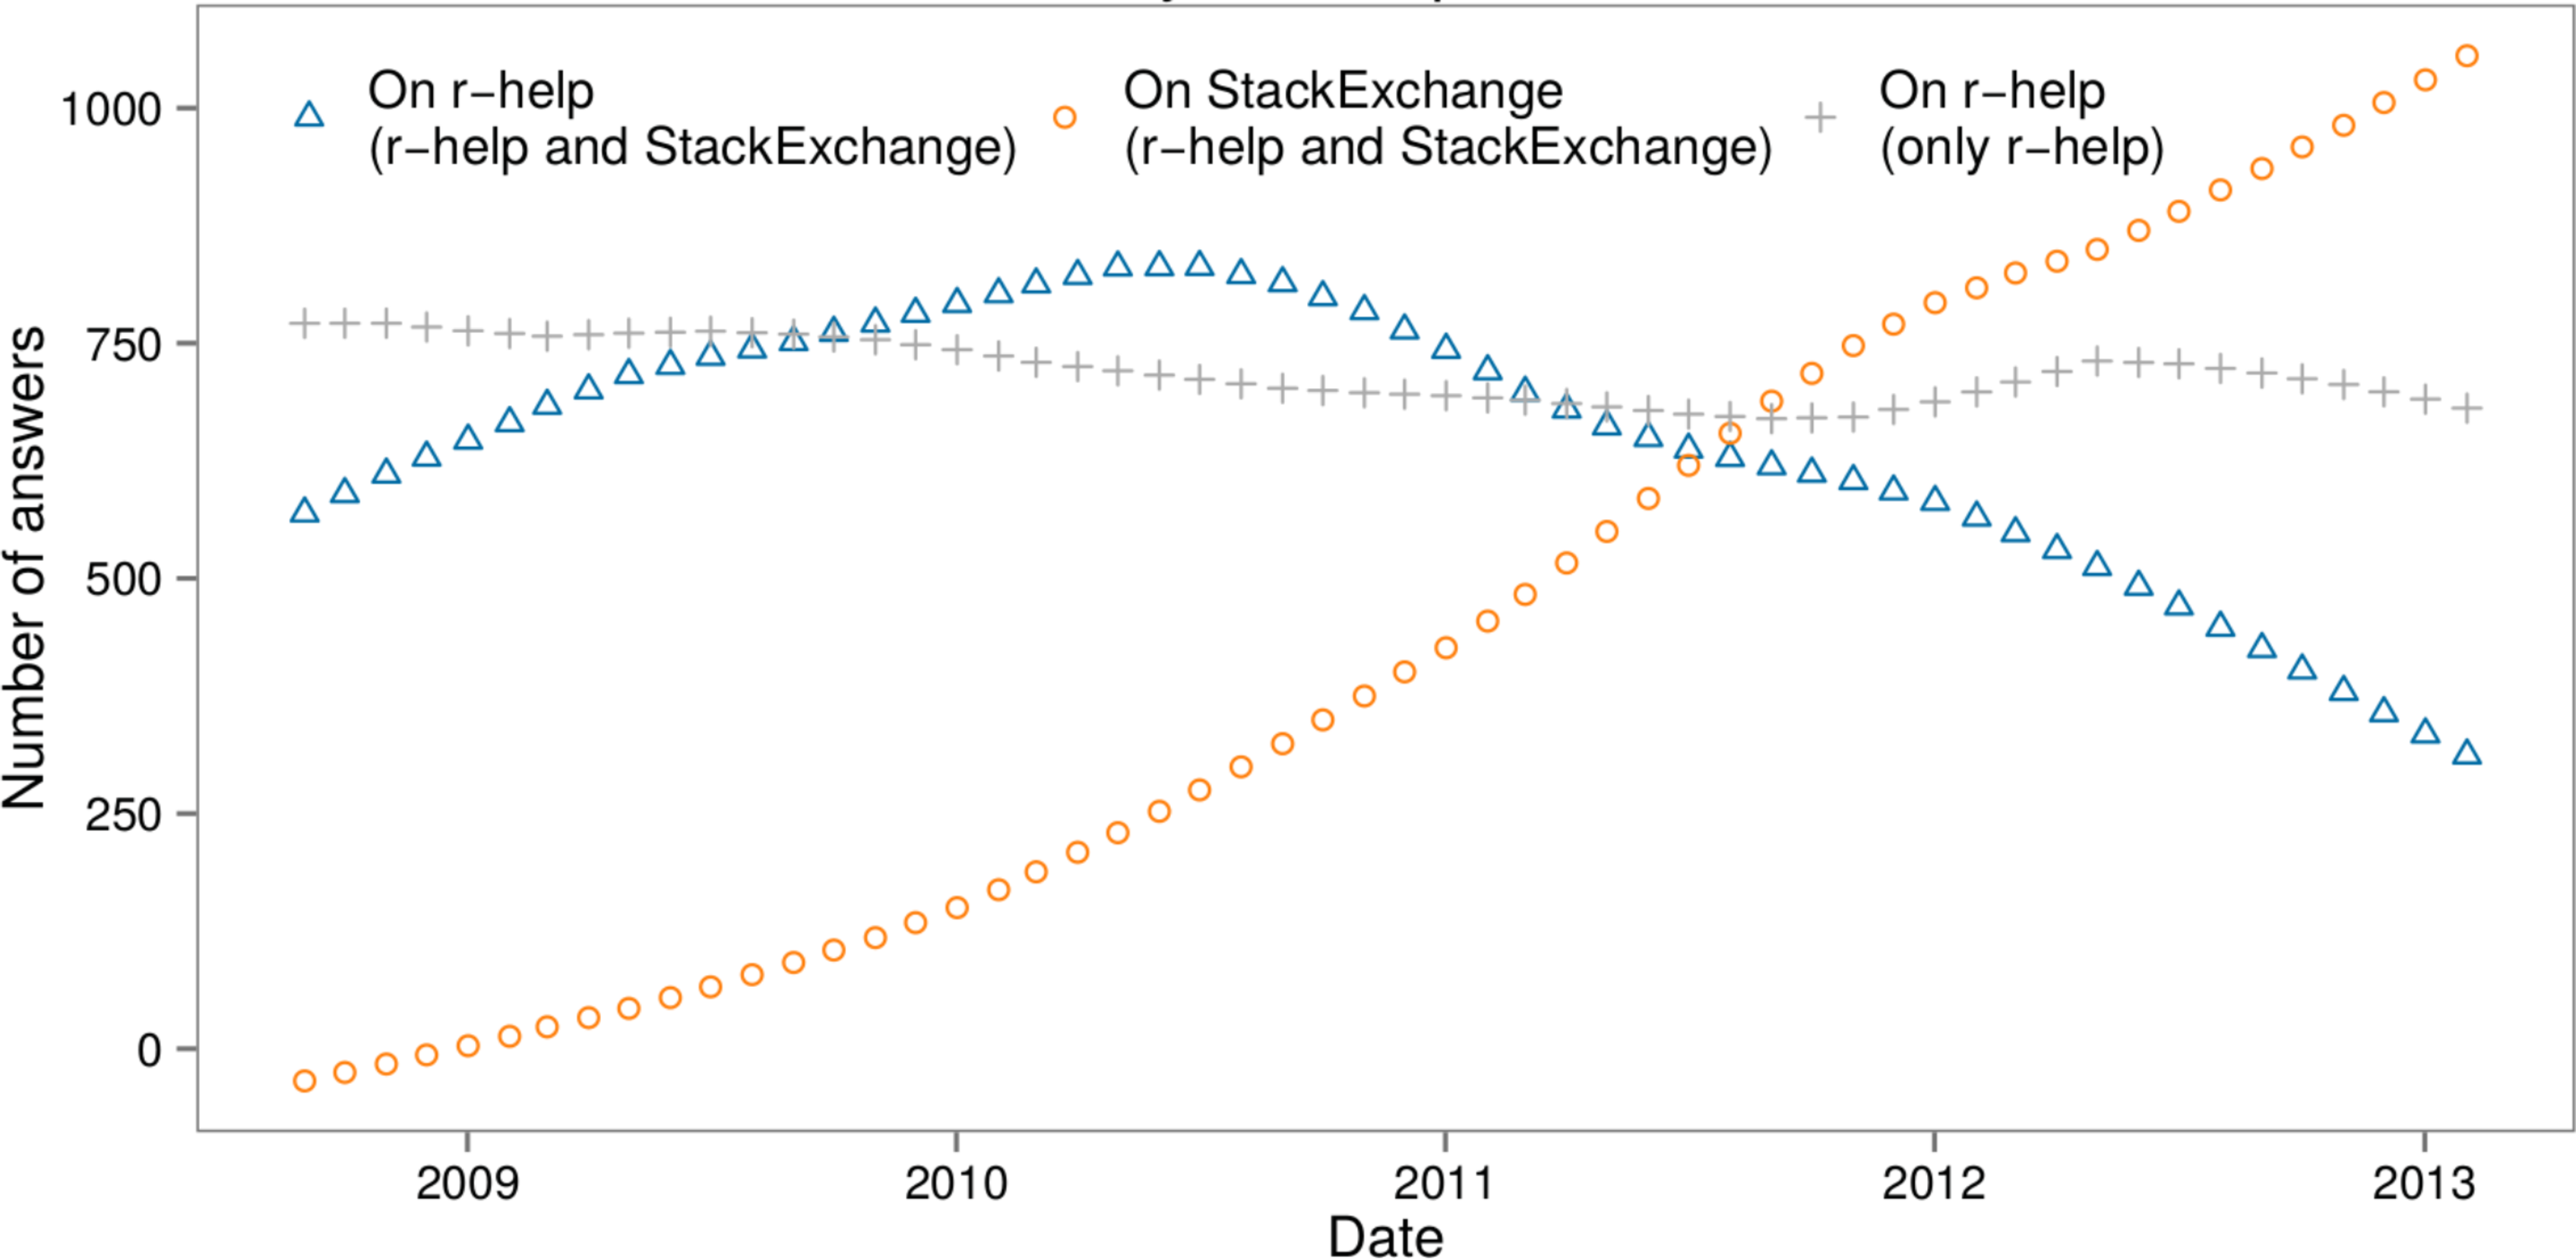
\includegraphics[width=1\columnwidth]{Figures/VasilescuFA2}
		\caption{(TOP) Number of questions asked (threads started) each month on R-help and Stack Exchange (Stack Overflow and Cross Validated)~\cite{Vasilescu2014c}. (BOTTOM) The number of questions answered on the R-help mailing list (after September 2008) and Stack Exchange each month: participants exclusive to the mailing list versus those also active on Stack Exchange~\cite{Vasilescu2014c}.}
		\label{fig:VasilescuFA1}
	\end{figure}


\section{Methodology}
\label{cha:methodology}

	This chapter describes the elements of the methodology, including the research questions, the adopted case study methodology, and the phases of the study.
	This chapter also outlines the procedure used to collect and analyse the data in this study.

%\subsection{Research Questions}

%	The four research questions that guided this thesis are:

%\paragraph*{RQ-1. What types of knowledge are shared on Stack Overflow and the R-help mailing list within the R community?}

%	In the R community, the R-help mailing list serves the same purpose as Stack Overflow.
%	This led to the question of \emph{what types of knowledge are shared on Stack Overflow and the R-help mailing list?}
%	To answer this question I proceeded to analyse and categorize the knowledge in questions, answers, updates, comments and flags on Stack Overflow and the R-help mailing list.
%	Based on the analysis I was able to contrast the way knowledge flows through Stack Overflow and the R-help mailing list.

%\paragraph*{RQ-2. How is the knowledge constructed on Stack Overflow and the R-help mailing list?}

%	As discussed before, Stack Overflow and the R-help mailing list support the R community. 
%	Such a statement implies that the interactions hosted by these two media channels are of a collaborative nature.
%	I wondered if the same applies to the creation and sharing of knowledge in these two channels.
%	My goal was to identify the mechanisms and strategies on Stack Overflow and the R-help mailing list used to construct knowledge collaboratively and individually (if any).

%\paragraph*{RQ-3. How does the sharing of links on Stack Overflow and the R-help mailing list support knowledge construction?}

%	On the Internet, links support the reuse and referencing of data from other resources.
%	Links contain information that is valuable for messages, and depending on how they are used, links can support knowledge sharing practices in different ways.
%	For instance, a link can expand what is known about a topic by referencing more complete sources of information, or provide data to reproduce certain behaviours on source code examples.
%    Previously, I have identified the types of links on Stack Overflow and how they support diffusion of knowledge~\cite{Gomez2013}.
%	For this study, I pursued the identification of how links contribute to the construction of knowledge.
%	Thus, I categorized links posted in the body of messages on Stack Overflow and the R-help mailing list based on their type (e.g., Q\&A Website, and Forums), and how each type of link supported the knowledge construction.

%\paragraph*{RQ-4. Why do certain users post to both Stack Overflow and the R-help mailing list?}

%	As mentioned by Vasilescu~\cite{Vasilescu2014b}, there is a group of users that are active on Stack Overflow and the R-help mailing list. 
%	I wondered if there were any advantages or disadvantages on using both channels.
%	With that in mind, I identified a list of active users in both channels and used open coding methods to analyse their posts.

\subsection{Case Study Methodology}

	As claimed by Yin~\cite{Yin2009,Yin2012}, a case study facilitates the exploration of a phenomenon within its context using a variety of data sources.
	In software engineering, a \textit{case study} is defined as  \textit{``an empirical enquiry that draws on multiple sources of evidence to investigate one instance (or a small number of instances) of a contemporary software engineering phenomenon within its real-life context, especially when the boundary between phenomenon and context cannot be clearly specified''}~\cite{Runeson2012}.

	According to Yin~\cite{Yin2012}, a case study should be used when: 
	(1) ``How'' or ``why'' questions are trying to be answered; 
	(2) the researcher cannot manipulate the behaviours of those involved in the study; 
	(3) the context is an important part of the study; 
	(4) there are no clear differences in what is happening between the phenomenon and the context; 
	and (5) when multiple sources of evidence have to be covered. 
	Because these conditions apply to the nature of this study and its research questions, I selected the case study methodology for this work. 
	Specifically, this thesis is an exploratory case study to explain the interplay of multiple media channels within a community in terms of the knowledge created and shared.
	%Our goal is to gain insights and compare the usage of selected media channels within the R community. \remarks{Check if this is the same everywhere}

	The study is divided in two phases that were performed in parallel: mining of data archives, and the survey.
	Figure \ref{fig:StudyPhases} depicts the general organization of the study design.
	In the next sections of this chapter, each phase is explained in detail.

	\begin{figure} [!ht]
		\centering
		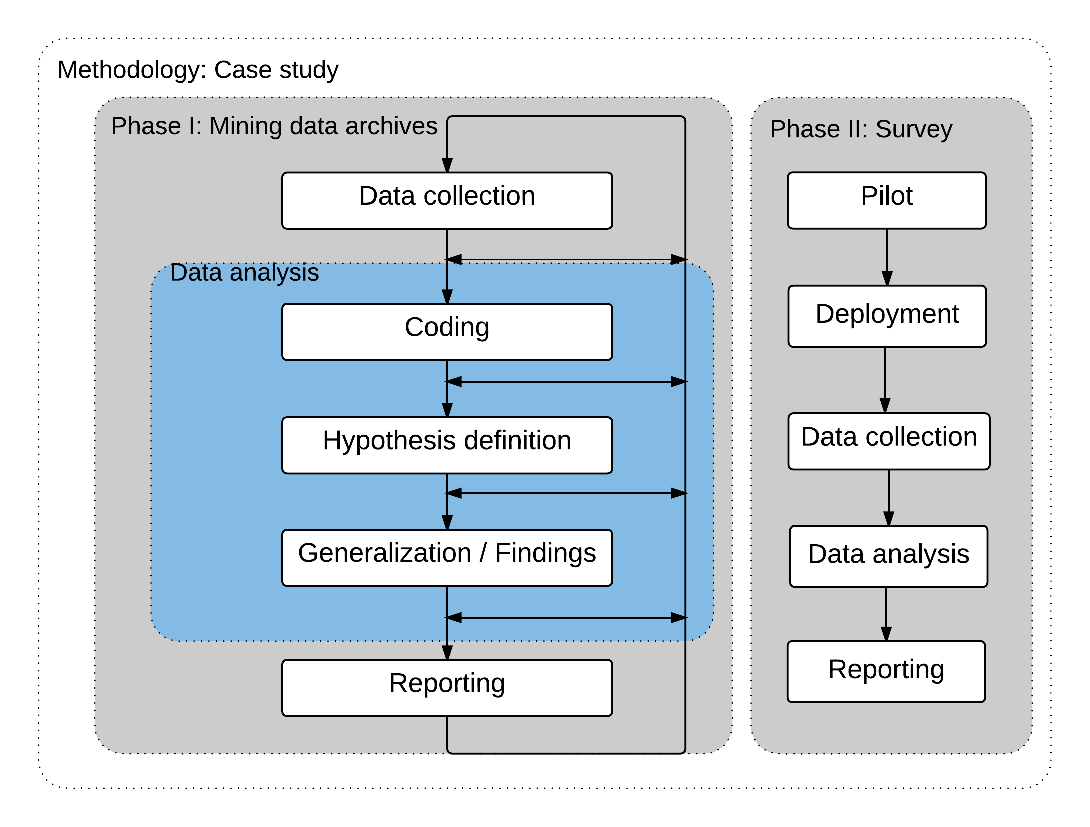
\includegraphics[width=0.9\columnwidth]{Figures/StudyPhases}
		\caption{General overview of the study design}
		\label{fig:StudyPhases}
	\end{figure}

\subsection{Phase 1: Mining Data Archives} 
\label{sec:studyDesign}

	The mining of the data archives method involved a three step process: data collection, data analysis, and reporting~\cite{Runeson2012}.
	The \textbf{data collection} step involved in gathering the body of data required for analysis. 
	This data was a selected set of R-related posts from Stack Overflow and the R-help mailing list.
	In the \textbf{data analysis} step, I analysed the data looking for answers for the research questions.
	Finally, the \textbf{report} step, consolidated the results, which are presented in Chapter~\ref{cha:findings}.

\subsubsection{Data Collection and Preparation}
\label{subsec:preparation}

	Stack Overflow and the R-help mailing list store their messages in publicly available archives.
	The records available for Stack Overflow start in 2008 (the birth of Stack Overflow), while the R-help archives go back to 1997.
	To make both data sets comparable, I analysed the data from 2008 until 2013, a period of time that both channels were available simoultaneously.

	Users can obtain Stack Overflow's archived message data using a variety of different mechanisms:
	(1) directly, through the Stack Overflow Website,
	(2) using Stack Exchange online query services, or
	(3) through a dump file\footnote{\url{https://archive.org/details/stackexchange}}, containing data from all the Stack Exchange Websites in XML format (a new version is released every three months).
	For this thesis, I used the data provided by the dump file.
	%<<
	The R-help mailing list data (i.e., emails sent to the list) is available through the R community Website as MBOX files organized monthly from April 1997 until January 2015.
	%>>

	To prepare the data, I used two software tools depending on the data set.
	(1) to process the Stack Overflow data, I used a modified version of Sam Saffron's application, So-Slow\footnote{\url{https://github.com/SamSaffron/So-Slow}}; and,
	(2) to process the R-help mailing list archives, I wrote a software application, based on the Bettenburg \textit{et al}~\cite{Bettenburg2009} recommendations of how to process mailing list data.
	I followed the process depicted in Figure~\ref{fig:data_extraction}.
	First, I extracted the archived data.
	Then, I used the aforementioned tools to pre-process the archive files, and then load the data into a database. 
	Next, I executed custom queries to obtain random samples data to analyse.

	\begin{figure}[!htb]
		\centering
		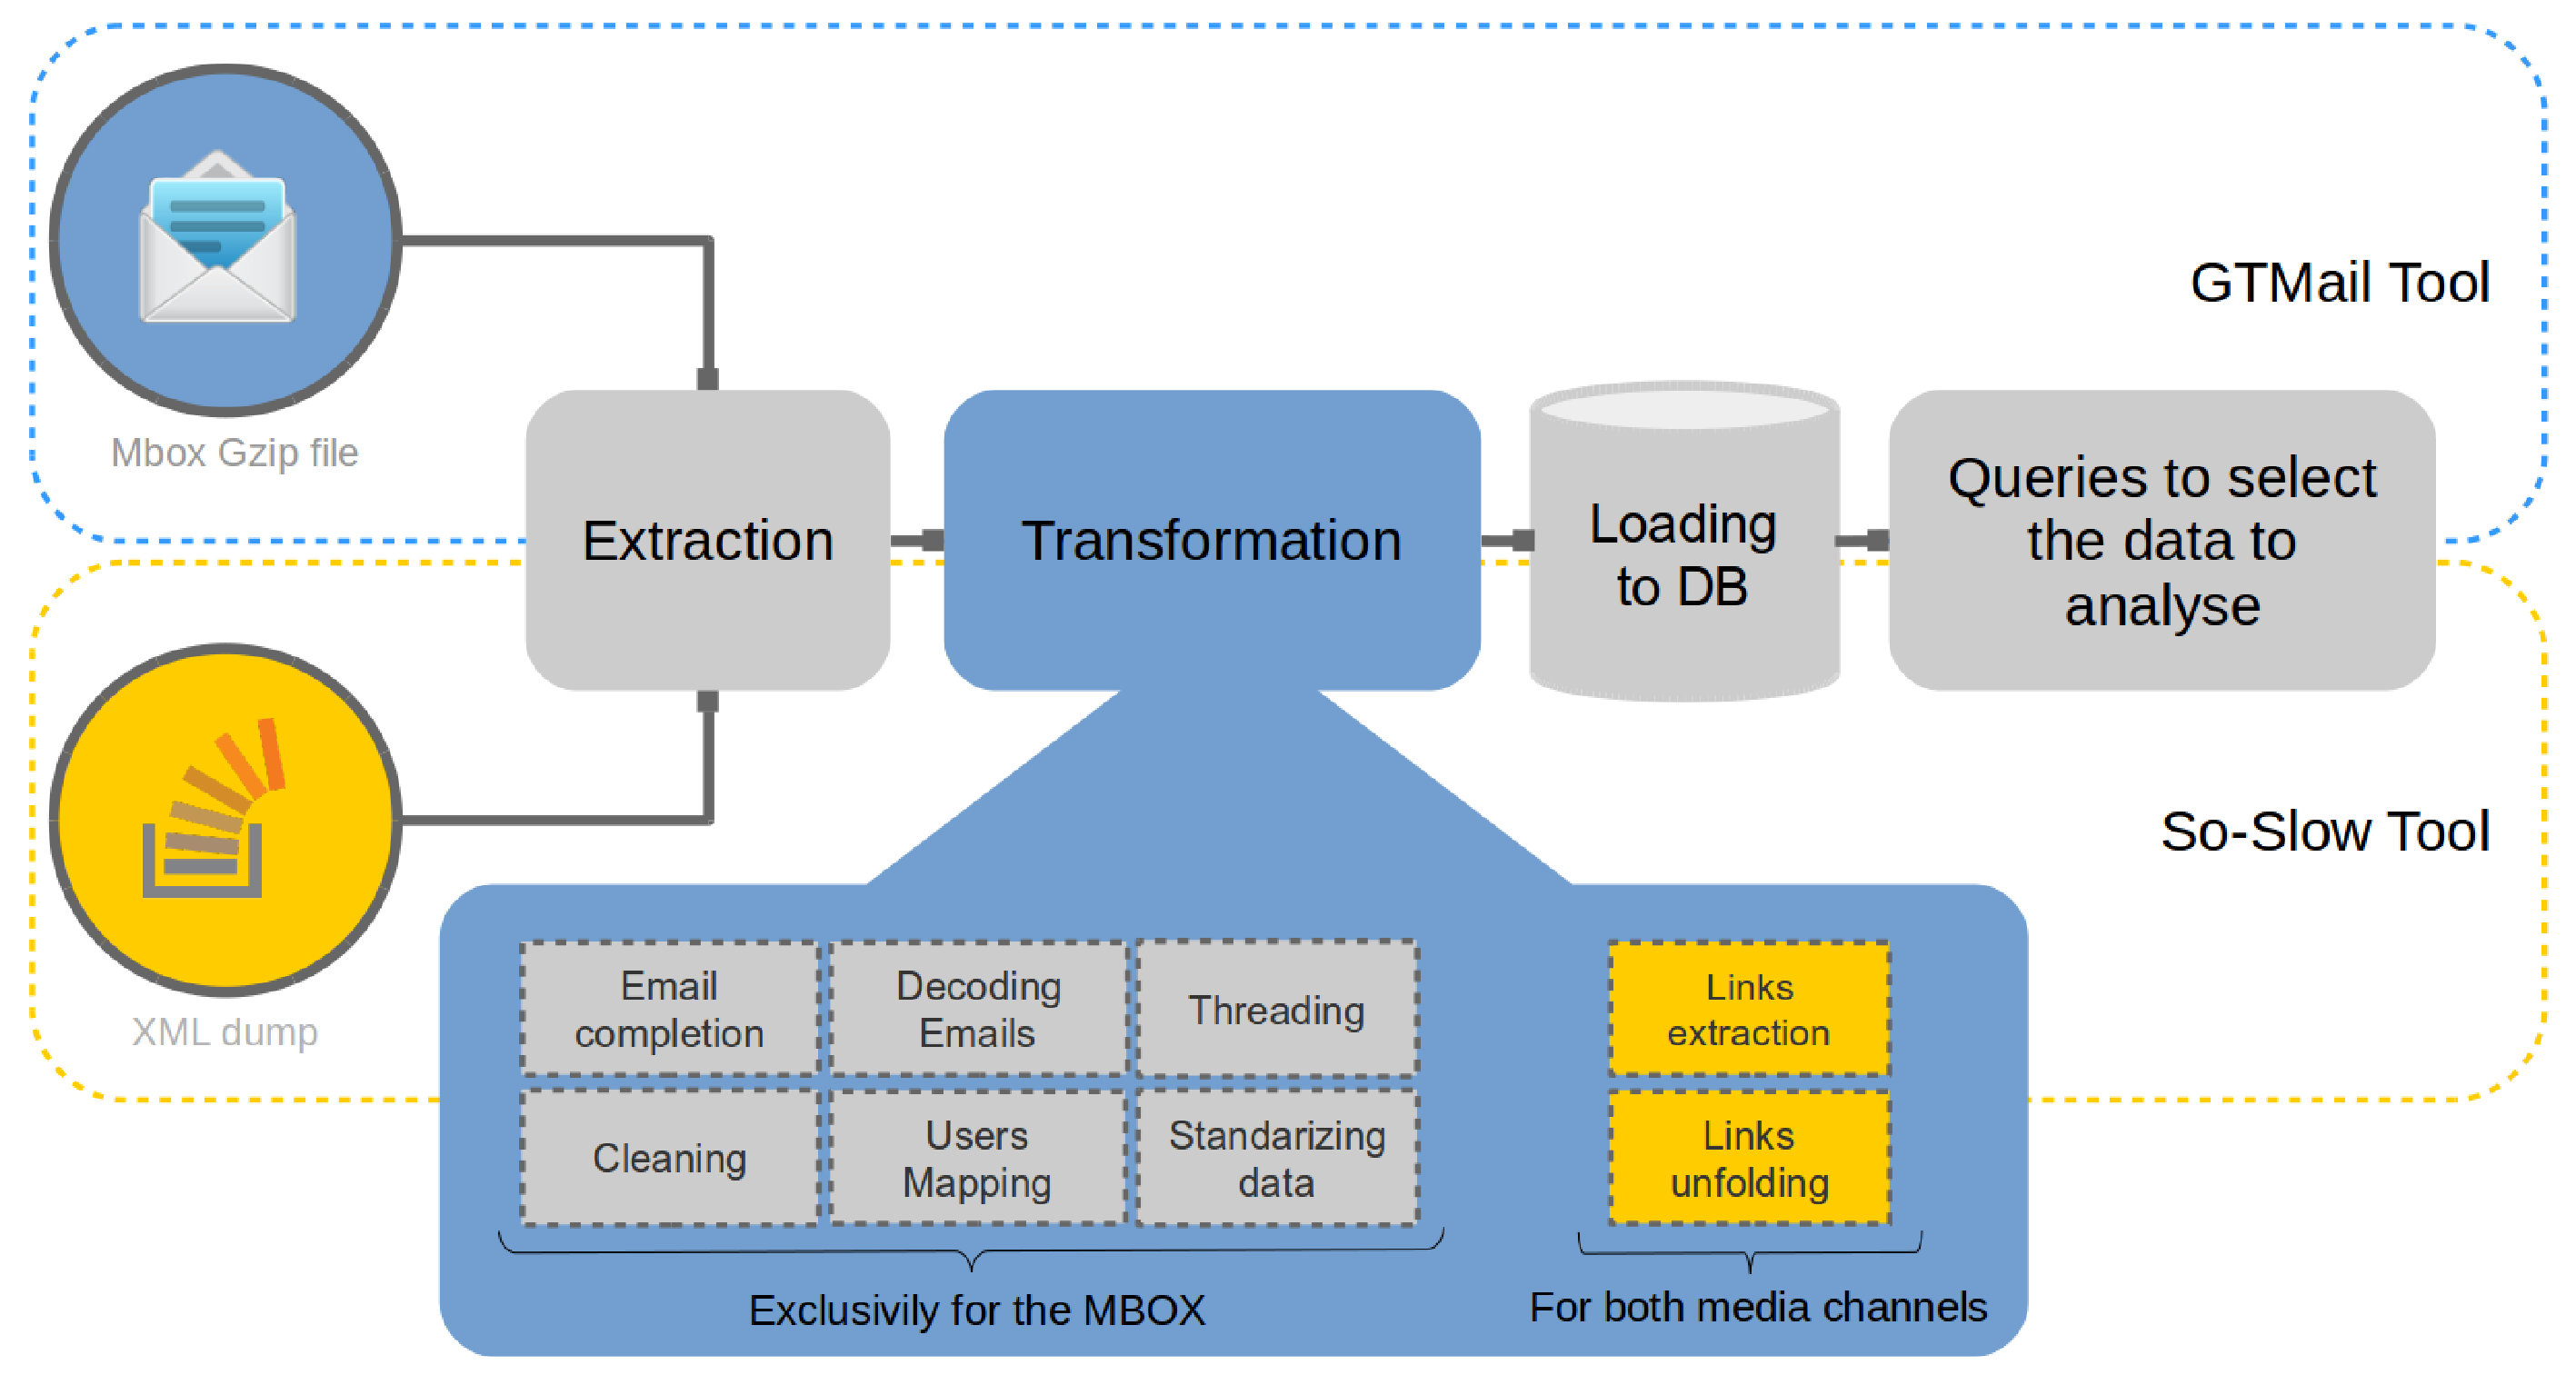
\includegraphics[width=\columnwidth]{Figures/data_extraction}
		\caption[Data process]{Process applied to the data of both media channels.}
		\label{fig:data_extraction}
	\end{figure}

	Table~\ref{table:data} depicts a summary of the data uploaded into the database. 
	The R-help has more questions, answers, and users than Stack Overflow, due the fact that there is approximately ten years of additional data.
	Only Stack Overflow's data contains ``comments'' information, so this field is empty for the R-help mailing list column.

	\begin{table}[!htb]
		\caption{Raw data collected for each channel.}
		\begin{center}
			\begin{tabular}{lrr}
				\toprule
				\multirow{2}{*}{Type} & \multirow{2}{*}{R-help} & Stack Overflow \\
				                      &                         & \multicolumn{1}{c}{(r---tag)}\\
				\midrule
				Questions     & 101,931 &  67,393 \\
				Answers       & 213,366 &  99,620 \\
				Comments      &       - & 286,124 \\
				Users         &  39,150 &  26,324 \\
				\bottomrule
			\end{tabular} 
		\end{center}
		\label{table:data}
	\end{table}

	The following subsections detail the analysis process for each media channel.

\subsubsection*{The R-help Mailing List}
\label{subsec:r-help}

	As stated earlier, the R-help archives are in the MBOX format. 
	However, the information inside of the email is still unstructured data.
	The MBOX format separates the metadata (header) from the content (body), but there is not a clear division between what are source code examples, the sender's message and signature, and other semantic elements that might exist on emails.
	The MBOX format only provides certain information about the email, such as the sender and receiver's email addresses, the subject of the email, and the emails on the thread.
	Figure \ref{fig:WellFormedEmail} depicts an example of a well-formed MBOX file.
	In the top, a clear defined information that can be extracted from the email (header), but the body is unstructured. To analyze the body, it has to be cleaned from noisy data such as signatures and quoting text.

	\begin{figure}[!htb]
		\centering
		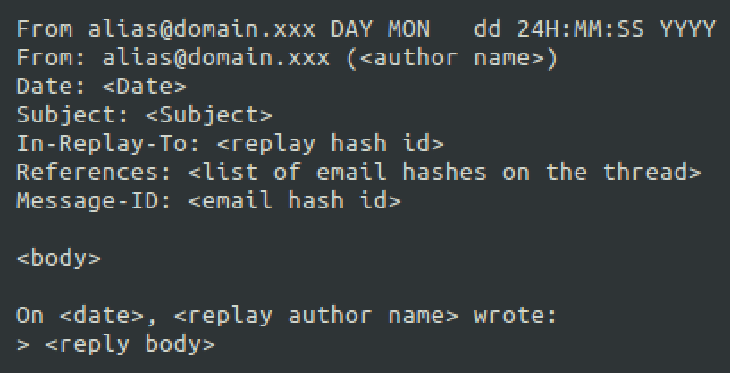
\includegraphics[width=0.8\columnwidth]{Figures/WellFormedEmail}
		\caption[Example of a well-formed MBOX file]{Example of a well-formed email in the MBOX format.}
		\label{fig:WellFormedEmail}
	\end{figure}

	Bettenburg \textit{et al}.~\cite{Bettenburg2009} proposed a series of recommendations for proper processing of mailing list data, to ensure accurate research results.
	In my search of existing tools, I found a couple used for research that handles MBOX data, such as Herraiz \textit{et al}. tool, MailingListStats\footnote{\url{https://github.com/MetricsGrimoire/MailingListStats}}, and REmail\footnote{\url{https://code.google.com/p/r-email/}} tool.
	However, I could not find evidence of how MailingListStats was constructed, or if it is resilient to MBOX format inconsistencies. While the REmail tool was meant for a totally different purpose--- to match source code with emails from projects' archives.

	To pre-process the R-help archives, I created a Java application based on Bettenburg's recommendations that:
	(1) standardizes the MBOX format considering spacing and email address formatting,
	(2) extracts information from the MBOX files like sender's date, subject and message,
	%<<
	(3) groups e-mails into threads using Jamie Zawinski's algorithm\footnote{\url{https://www.jwz.org/doc/threading.html}} which provides support for sub-threading (threads that might exist at the inside of a main thread),
	%>>
	(4) removes duplicated emails,
	(5) removes URLs in footnotes and signatures,
	(6) reconstructs threads when neither \textit{Reference} nor \textit{Reply} appear in th header, but the body of the message shows text from previous emails (for this purpose, I matched e-mails by subject and organized them by arrival time),%---Figure \ref{fig:Thread} depicts an example of a thread to highlight the complexity of the reconstruction);
	(7) extracts URLs and unfolds shortened URLs,
	(8) downloads emails with coding problems from the URL left by the mailing list server after scrubbing the body,
	(9) solves text encoding issues (i.e., text that it is not in UTF-8 format),
	(10) transforms the email addresses to MD5 hashes,
	(11) changes the creation date (the R-help mailing list time zone is UTC+2) to UTC (Stack Overflow's server time),
	and (12) uploads the data to our database.
	Figure \ref{fig:ML-ERD} depicts the entity--relational model used to store the data from the mailing list.

	\begin{figure} [!ht]
		\centering
		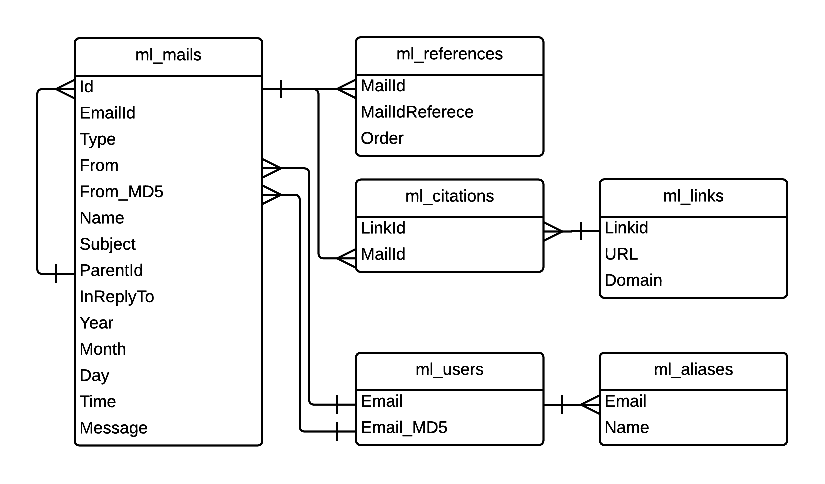
\includegraphics[width=\columnwidth]{Figures/ML-ERD}
		\caption{Entity Relation Diagram of the R-help mailing list data.}
		\label{fig:ML-ERD}
	\end{figure}

\subsubsection*{Stack Overflow}
	% time zone of the mailing list is UTC
	%Update on the table
	Every three months, Stack Exchange releases a new data dump file in XML format that contains data from all their Websites\footnote{\url{http://stackexchange.com/sites}}.
	However, the last dump file containing email addresses as MD5 hashes was released in September 2013--- 
	the Stack Overflow dump files produced after September 2013 do not provide users' email addresses.
	The email hashes were used to match users from Stack Overflow with users in the R-help mailing list. 
	This technique was used to answer RQ4 and is explained later in this chapter.
	Because of this, I used the data dump file from September 2014, but updated the table \texttt{users} with the hashes in the dump file from September 2013, for whose \texttt{ID}s were identical in both data sets.
	In case a user from the 2013 data file did not exist in the 2014 data (e.g., as consequence of the \textit{right to be forgotten}\footnote{\url{https://en.wikipedia.org/wiki/Right\_to\_be\_forgotten}}), I ignored the user.

	As stated previously, I used a modified version of Sam Saffron's application, So-Slow.
	The purpose of this is to extract the information in the file using XML tags (e.g., post, user, and comment), and load it in a database.
	I filtered all R-related data by selecting only messages with the R tag (i.e., \texttt{r}) and its synonyms\footnote{\url{http://stackoverflow.com/tags/r/synonyms}} (i.e., \texttt{rstats} and \texttt{r-language}).
	Figure \ref{fig:SO-ERD} depicts the entity--relational model used to store the Stack Overflow data.

	\begin{figure} [!ht]
		\centering
		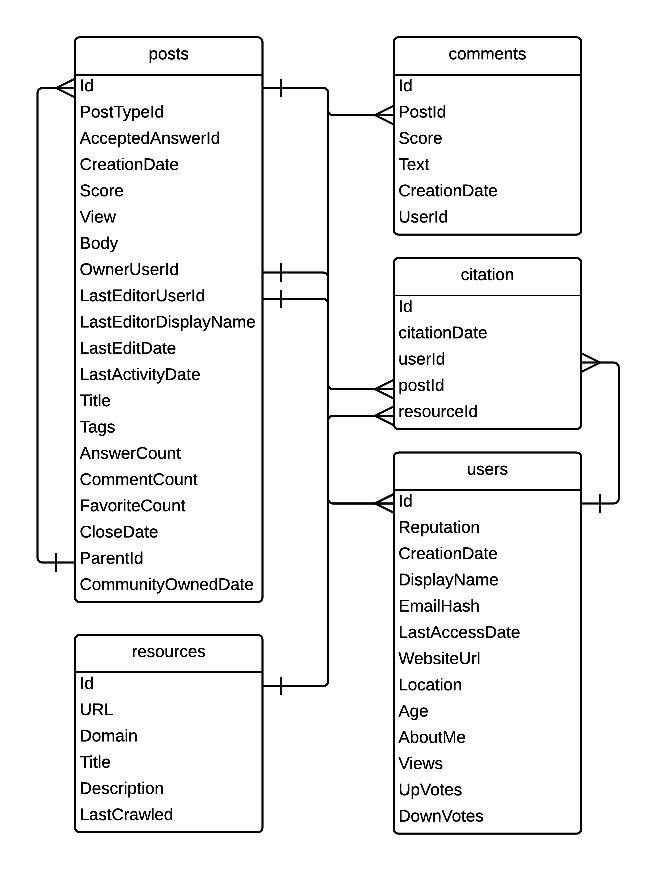
\includegraphics[width=0.8\columnwidth]{Figures/SO-ERD}
		\caption{Entity--Relation Diagram of the Stack Overflow data.}
		\label{fig:SO-ERD}
	\end{figure}

\subsubsection*{Data Merging}
	There are some studies that propose different techniques for merging users' identities by analysing the data from multiple repositories (e.g., mailing lists, bug tracking information, and source code management tools)~\cite{Bird2006, Kouters2012,Vasilescu2014c}.
	Bird \textit{et al}.~\cite{Bird2006} proposed a heuristic to match users' identities across multiple mailing list archives by combining parts of user names and email addresses. For example, the \textit{cagomezt} prefix is likely to belong to \textit{Carlos Arturo Gomez Teshima}.
	Furthermore, Kouter \textit{et al}.~\cite{Kouters2012} used a natural language processing technique called Latent Semantic Analysis to merge identities on very noisy data.
	However, it has been demonstrated that all existing approaches produce false positives and false negatives~\cite{Goeminne2013}.

	For this work, I used the approach proposed by Vasilescu \textit{et al}.~\cite{Vasilescu2014c}, which is the most conservative technique considering the available data~\cite{Vasilescu2014b}---it does not use any method to infer email addresses based on user name.
	Vasilescu's technique consists of matching Stack Overflow's email MD5 hashes with the MD5 hash version of email addresses from the R-help mailing list data.
	With this technique, the resulting set included 1,421 different users with the same email address on both media channels.

	Because Stack Overflow only provides the email addresses as MD5 hashes, and to make both data sets comparable, the mailing list emails were converted to their corresponding MD5 hashes.

	It is important to note that MD5 hashes are not \textit{collision resistant}\footnote{\url{https://en.wikipedia.org/wiki/Collision_resistance}} and therefore, this could possibly lead to false positive resistant outcomes. 
	However, it is unlikely for two different email addresses to share a MD5 hash.
	According to the Request for Comment (RFC) 1312\footnote{\url{https://www.ietf.org/rfc/rfc1321.txt}} from the Internet Engineering Task Force (IETF), the probability to find a MD5 collision is less than $1/2^{64}$.

\paragraph{Data Analysis Process}
\label{sec:dap}

	I used a qualitative data analysis approach to study the data that flows through Stack Overflow and the R-help mailing list.
    A qualitative and exploratory approach best suits research when a concept or phenomenon requires more understanding, since there is little pre-existing research~\cite{Creswell2009}.

	In particular, I used the inductive approach of Runeson \textit{et al}.~\cite{Runeson2012} to analyse the data from Stack Overflow and the R-help mailing list.
	This approach is iterative, across the study it is necessary to switch between data selection and data analysis, or between data reporting and data collection.
	To reduce bias, it is advised the involvement of multiple researchers~\cite{Runeson2012}.
	As a consequence, this study was conducted by two researchers, both computer scientists with a background in qualitative data analysis.

	%<<
	\begin{figure} [!htb]
		\centering
		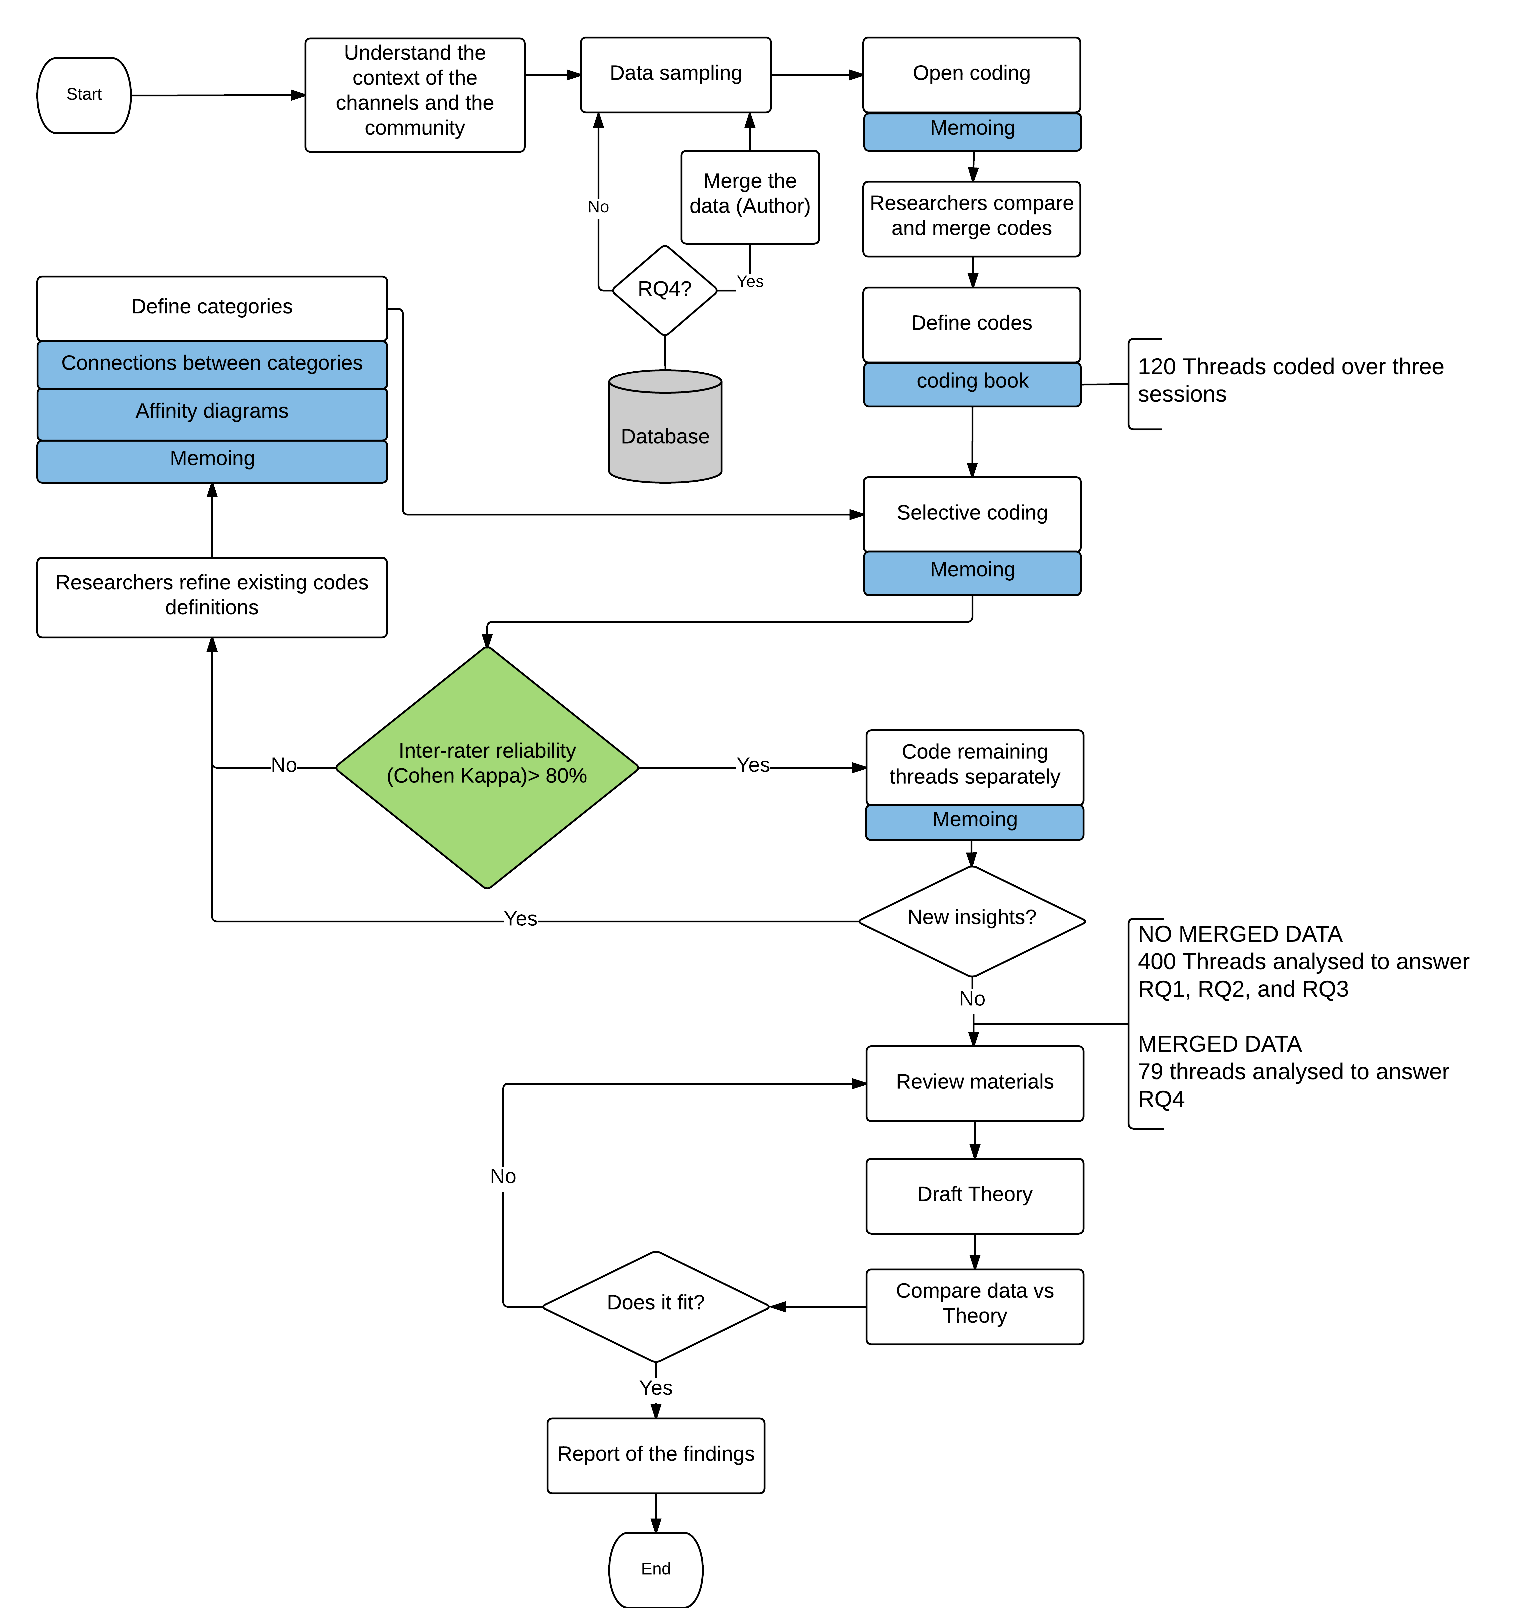
\includegraphics[width=1\columnwidth]{Figures/ContentAnalysisFlow_3}
		\caption[Our content analysis method]{Qualitative approach used to analyse Stack Overflow and the R-help mailing list data. This chart shows the process and techniques (coloured figures) used to analyse and develop the findings of this work.}
		\label{fig:ContentAnalysisFlow}
	\end{figure}
	%>>

	Figure \ref{fig:ContentAnalysisFlow} depicts a visual explanation of the data analysis process for this study.
	My colleague and I refined our codes and categories by repeating numerous times the process of collecting and analysing the data.

	The next sections, for the sake of clarity for the reader, have been presented in a linear fashion. 
	However, the process as depicted in Figure \ref{fig:ContentAnalysisFlow} is not linear. 

\paragraph{Techniques Used to Support the Analysis}
	Figure~\ref{fig:ContentAnalysisFlow} contains some coloured shapes that depict the techniques used to support the data analysis, which are explained as follow:

	\begin{itemize}
		\item \textbf{Memoing} refers to the act of taking notes (coding) about what the researcher is learning from the data during the analysis~\cite{Groenewald2008}, for example, the hypotheses regarding a code, and relationships between concepts.
		During this stage, reflective memos were written in a spreadsheet next to the applicable codes as the researcher coded (see figure \ref{fig:CodingExample}).
		These memos were used to create the codes, and hypotheses about the relationships between concepts.

		\item \textbf{Affinity diagrams} is a technique that allows one to organize ideas and data into groups and to find the relationships between concepts~\cite{Scupin1997}.
		During the study I used affinity diagrams when discussing new insights with my colleague, and while defining categories and relationships between them.

		\item \textbf{Inter-rater agreement \textit{Cohen Kappa}} is a coefficient used to measure the agreement between two coders who classify items into mutually exclusive categories~\cite{Stemler2004}.
		Ladis and Koch suggest that values above 0.60 or 60\% to obtain substantial results~\cite{Landis1977}.
		In a previous study~\cite{Gomez2013}, we used the same coefficient to measure agreement between coders.
		Based on this experience, I set a value above 0.80 or 80\% as the minimum to obtain substantial results.
		%<<
		In this study, I used the Cohen Kappa coefficient after each coding session as a way to trigger discussion.
		%>>

		\item \textbf{Code book} is the book that contains the definitions of the codes that the researchers look during the data analysis~\cite{MacQueen1998}.
		Codes are the building blocks for theory and foundations on which the researcher's argument rest.
		We coded an initial set of 120 threads over three sessions.
		In each session, my colleague and I separately coded 40 threads.
		The multiple sessions allowed us to refine definitions in the codebook.
		Each entry in the code book is associated with a title, a formal definition, an example, and space for notes from the researcher.
		The final version of the codebook with the corresponding categorizations are detailed in Chapter~\ref{cha:findings}.
	\end{itemize}

\paragraph{The Analysis Process}

	The focus of the analysis is to \textit{understand the context of the media channels and the community}.
	The process consisted of:
	First, a recollection of the official information for both channels and the community to build a background of the community of practice and the channels studied.
    From the channels, I collected posting guides, rules, channel objectives, and competitors, whereas from the community I collected the number of members, how it works, and the media channels that the community uses.

	Second, a mapping between messages from Stack Overflow (i.e., question, answer, update, comment, and flag) with messages on the R-help mailing list.
    This is to overcome how the data is structured in both channels.
    Stack Overflow has a clear delimitation of what is a question, an answer, a comment, a flag and an update, while the R-help mailing list is just plain text.
    The mapping of messaged between both channels was as follows:

	\begin{itemize}
		\item \textbf{Question:} the message is the first on the thread, and it contains the main question.
		\item \textbf{Answer:} the message provides a solution to the main question of the thread.
	 	\item \textbf{Update:} the message claims for a modification to a question (or answer) made by the author of such a question (or answer).
		\item \textbf{Comment:} the message offers a clarification to a specific part of the question or answer.
		\item \textbf{Flag:} the message requests attention from the moderator (e.g., repeated questions, spam, or rude behaviour).
	\end{itemize}

	Next, for the \textit{data sampling} step, to answer RQ1, RQ2 and RQ3, I used a simple database query that selected a time frame and randomly returned threads from each channel.
	%<<
	The data set was capped at 400 threads for each channel (0.4\% and 0.6\% of the data available at the time of writing this thesis for the R-help mailing list and Stack Overflow respectively), when my collaborator and I deemed our observations as being saturated.
	To answer RQ4, I used the same query as before, but I added a condition that matched, on both channels, messages with the same subject written by the same author (we merged the data).
	%>>
	Given that only 79 threads were returned from this query, my colleague and I analysed the entire population available. 

	To code the data, we used an \textit{open coding} technique that involves reporting \textit{what the researcher saw} during each coding session. 
	The researcher has to keep in mind, all the time, the objective of the study and perform the coding based on it.
	Each researcher coded the data on a separated way.
	During the coding session, we wrote memos as needed, and marked repetitive patterns.
	Later, we met to compare and discuss findings, and begin developing codes.

	From our initial codes, we began the process of creating a \textit{coding book} to outline definitions. 
	This set of codes were used later during the \textit{selective coding} step.
	At this point, the researcher stops coding every occurrence, and begins seeing larger trends and connections within the data and codes.
	It is possible that during the \textit{selective coding} step some codes have to be reformulated, or maybe split into more codes. 
	Also, it is possible to formulate completely new codes as needed.
	Whenever there is a new code or any is changed, it is necessary to go back and recode the material.

	As a coding tool, my colleague and I used a spreadsheet in which each row represents a message of the thread.
	%<<
	If for any reason a message appeared to fit in more than one category, each researcher selected, at their own discretion, a primary category to represent the message.
	%>>
	Figure~\ref{fig:CodingExample} depicts an example of the coding spreadsheet that we used.
	The number in the first column identifies if the message is a question, an answer or a comment. 
	For instance, if the number assigned to the question was ``1'', then the answers were enumerated with consecutive numbers separated by a point (e.g., 1.1); and the comments were enumerated in a similar way to enumerated answers, but using three numbers: the first number represents the question, the second represents the answer, and the third represents the comment consecutive (e.g., 1.0.1). 
	The second column contains the message, the third column the channel, the fourth column the question categorization, and so on.
	The last column contains the URL to the thread on the channel.
	Inside each cell, a semicolon ($;$) represents a sub-category, and the double pipe ($||$) divides two different ideas (e.g., in the \textit{MEMOS} column), or indicates that a message was re-classified after an update (e.g, \textit{ANSWER} column).

	At the beginning of the coding, before we created the code book, the spreadsheet had only the \textit{ID}, the \textit{MESSAGE}, the \textit{MEMOS}, and the \textit{URL} columns.
	During each iteration, the spreadsheet was updated with the classification and type of messages that my colleague and I were defining.

	Originally, both researchers read the threads directly from the spreadsheet.
	However, this method of reading turned out uncomfortable, and we fell back to read the threads directly from each channel rather than the spreadsheet.

%	\begin{landscape}
	 	\begin{figure}[!ht]
			\centering
			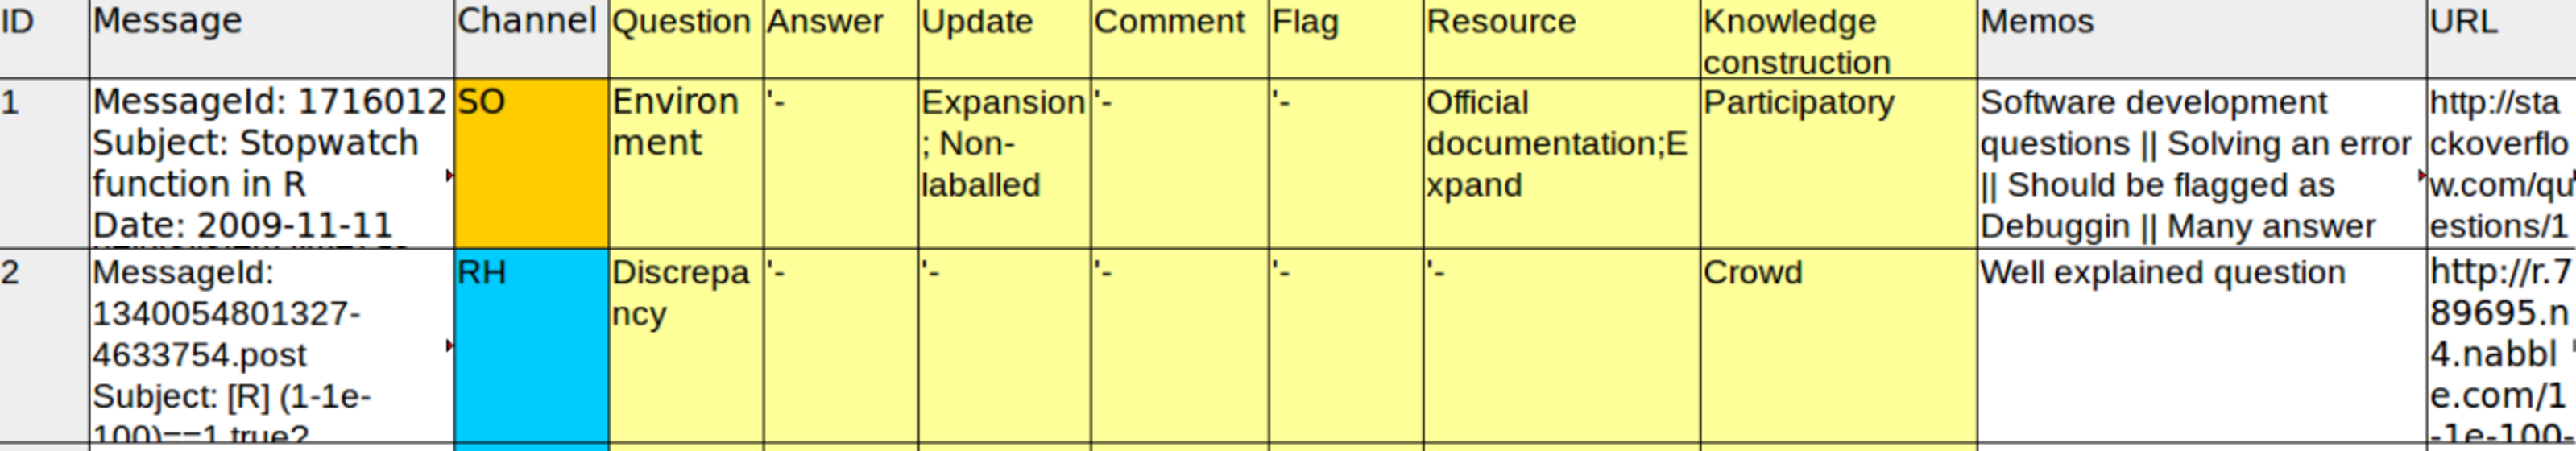
\includegraphics[width=1\columnwidth]{Figures/CodingExample}
			\caption[Example of how we coded the data]{Example of the way we coded the data. Each row of the spread sheet represents a message of the thread. Questions, comments, and answers can be identified with the number on the first column. The columns in yellow contain the codification for each message type. The last two columns contain the memos and the URL of the thread.}
			\label{fig:CodingExample}
		\end{figure}
%	\end{landscape}

\subsection{Phase 2: The Survey} 

	In \textit{phase 2}, I conducted a survey\footnote{A copy of the survey is published in \url{http://goo.gl/mxmH5J}} with members of the R community with the purpose of obtaining additional insights on the findings.
	First, I created a draft of the survey and did two pilots:
	(1) with colleagues in our research group, and
	(2) with R users at the University of Victoria.
	The objective was to test and refine the questions, tone, rankings, and the format of the survey.
	The survey questions were structured into five sections:
	(1) the user,
	(2) Stack Overflow use,
	(3) the R-help mailing list use,
	(4) Stack Overflow and the R-help mailing list if both used, and
	(5) resources linked to used.
	Survey's sections 2, 3 and 4 would only become active if the participant was a user of the channel.

	I announced our survey on Twitter, Reddit, the R-help mailing list, and Meta Stack Exchange to reach users of both channels, and minimize the selection bias. 
	However, on Stack Exchange the announcement was not well received and therefore was deleted a few minutes later after posting it.
	I received 26 valid responses out of 32 from the R community members.
	The survey did not collect any personal information.


\section{Findings}
\label{cha:findings}

	This chapter presents:
	(1) a characterization of the non-mutually exclusive categories and properties of Stack Overflow and R-help mailing list according types of knowledge the channels contains;
	(2) remarks about the ways knowledge is constructed on these two media channels;
	(3) an explanation of how links support the construction of knowledge;
	(4) a characterization of the knowledge based on the analysis of active users using both channels; and
	(5) interesting remarks about users regarding their behaviour on these two media channels.

\subsection{RQ-1. What types of knowledge are shared on Stack Overflow and the R-help mailing list within the R community?}
%\section{Types of Knowledge}
\label{cha:findings-types}

	As mentioned above, the R-help is not a specialized mailing list, therefore we were motivated to investigate whether Stack Overflow shares the same types of knowledge as R-help.
	As a result, we were able to identify that the messages from the Stack Overflow R tag and R-help mailing list contain five types of knowledge:
	(1) Questions;
	(2) Answers;
	(3) Updates;
	(4) Flags;
	(5) Comments.

\subsubsection*{Questions}

	Questions express one or more problems or doubts that a Stack Overflow or R-help user is experiencing.
	Through our coding my colleague and I identified 10 type of categories related to questions.
	This is explained as a result of the analysis of the R-help mailing list that by definition is more flexible on the topics allowed on the channel (e.g., announcements)

	Our 10 categories related to \textit{questions} are:
	\begin{enumerate}[\bfseries (1)]
	\item \textbf{How-to}: Questions that ask how to do something specific.
	\item \textbf{Bug/Error/Exception}: Questions that ask for a solution or reasons for a error message.
	\item \textbf{Discrepancy}: Questions that ask about an unexpected result of a specific function, process, or package.
	\item \textbf{Set-up}: Questions that ask for possible ways to set up the R environment before or after deployment.
	\item \textbf{Decision help}: Questions that ask needs help making a decision.
	\item \textbf{Conceptual/Guidance}: The user requests a conceptual clarification or guidance on topics related with R or statistics.
	\item \textbf{Code reviewing}: Questions that ask for a code review explicitly or implicitly.
	\item \textbf{Non-functional}: Questions that ask for help (or suggestions) with a non-functional requirement such as performance, and memory usage.
	\item \textbf{Future reference}: Questions that users ask---and normally answered themselves---that might not exist on the channel, but that are interesting enough to create a thread as a future reference.
	\item \textbf{Other}: Questions that ask for other assistance (i.e., questions not related to the channel) or the message contains unrelated information (e.g., announcements, ideas for improvement).

	\end{enumerate}

%	Table \ref{table:questions} shows examples from each channel for every type of knowledge shared through questions.%\remarks{I'm not sure about the use of USER in all the descriptions. I would rewrite them to remove the term, but that's me. If you stick with this format, should you differentiate between the user that posts a question vs the users that post answers, etc? Perhaps it's not important. Maybe ask Peggy.}

%	\begin{footnotesize}
%		\begin{longtable}{|p{3.9cm}|p{5cm}|p{5cm}|}
%			\caption{Examples of questions from both channels by type of knowledge.}
%			\label{table:questions}
%			\tabularnewline
%			\hline \textbf{Type of Knowledge} & \textbf{Stack Overflow} & \textbf{R-help} \tabularnewline

%			\hline \hline \textbf{How-to}
%			& \textit{``...Does anyone know a way of subsetting those 3 months of the time series?...''} {\footnotesize URL: \href{http://goo.gl/C5g1F3}{Q6356829}\footnote{URL transformation for StackOverflow: QXXXXXXXX where XXXXXXXX is the id of the question, such that http://stackoverflow.com/questions/XXXXXXXX/}}
%			& \textit{``...but I can't figure out how to resize each panel along the y axis and show only categories that have corresponding x values in each panel...''} {\footnotesize URL:  \href{http://goo.gl/Qat1yH}{QQat1yH}\footnote{URL transformation for R-help mailing list: QYYYYYY where YYYYYY is the URL shortened id, such that http://goo.gl/YYYYYY}} \tabularnewline

%			\hline \textbf{Bug / Error / Exception}
%			& \textit{``I'm getting a weird error when training a glmnet regression...''} {\footnotesize URL:  \href{http://goo.gl/6m1xwX}{Q1712316}}
%			& \textit{``Gives the error messages: Error in coxme.varcheck...''} {\footnotesize URL:  \href{http://goo.gl/KkYBe6}{QKkYBe6}} \tabularnewline

%			\hline \textbf{Discrepancy}
%			& \textit{``...But for some reason, a lot of lines get merged -- e.g., in row 500 of my data frame, I'll see something like...''} {\footnotesize URL:  \href{http://goo.gl/8kyzpR}{Q1407647}}
%			& \textit{``When I use wilcox.test, I get vastly different p-values than the problems from Statistics textbooks''} {\footnotesize URL:  \href{http://goo.gl/nXVLyD}{QnXVLyD}} \tabularnewline

%			\hline \textbf{Set-up}
%			& \textit{``When running Sweave from emacs-ess, errors are provided with a code chunk number. Is there an easy way to navigate among the code chunks by number?...''} {\footnotesize URL:  \href{http://goo.gl/cRV3nt}{Q4501404}}
%			& \textit{``Hi, exist any way to create a windows installable package from a Linux R installation''} {\footnotesize URL:  \href{http://goo.gl/cOHVdp}{QcOHVdp}} \tabularnewline

%			\hline \textbf{Decision help}
%			& \textit{``I have been asked to change a software that currently exports .Rdata files so that it exports in a 'platform independent binary format' such as HDF5 or netCDF...''} {\footnotesize URL:  \href{http://goo.gl/fu4Wqg}{Q7838027}}
%			& \textit{``I have two time series. Both measure the same thing and I would like to determine which one is noisier...''} {\footnotesize URL:  \href{http://goo.gl/ytDnBU}{QytDnBU}} \tabularnewline

%			\hline \textbf{Conceptual / Guidance}
%			& \textit{``What are some practices I can adopt so that my code will always be a pleasure to work with? I'm thinking about things like''} {\footnotesize URL:  \href{http://goo.gl/G5HrAc}{Q1266279}}
%			& \textit{``I would like to understand what are the units defined on the y-axis when you plot the one-dimensional predictions (histograms) from lda() (MASS) discriminant function objects?...''} {\footnotesize URL:  \href{http://goo.gl/kaP4Up}{QkaP4Up}} \tabularnewline

%			\hline \textbf{Review}
%			& \textit{``I'm trying to get all five outputs from the 5 data frames within the list x at the same time, but I am stuck here...''} {\footnotesize URL:  \href{http://goo.gl/QiNeN4}{Q17998174}}
%			& \textit{``...ghyp package and simulated series of t-distributed variables when suddenly i was not able to reproduce the log likelihood values reported by the package...''} {\footnotesize URL:  \href{http://goo.gl/H8GFiU}{QH8GFiU}} \tabularnewline

%			\hline \textbf{Non-functional}
%			& \textit{``The best implementation I could come up with uses a nested-loop, which I realize is probably the least efficient,...There must be a more efficient way of doing this?''} {\footnotesize URL:  \href{http://goo.gl/xj9Q3B}{Q1510039}}
%			& \textit{``...is there a better or more efficient way of doing this, maybe with apply or something...''} {\footnotesize URL:  \href{http://goo.gl/djtmdC}{QdjtmdC}} \tabularnewline

%			\hline \textbf{Future reference}
%			& \textit{``...I know the answer and I already tend to avoid sapply. I just wish there was a nice answer here on SO so I can point my coworkers to it. Please, no "read the manual" answer...''} {\footnotesize URL: \href{http://goo.gl/fA4dq6}{Q12339650}}
%			& \textit{``I've just posted a demo made with the rgl package to Youtube, visible
%			here: \href{http://goo.gl/vBWksU}{[link]} For future reference, here are the steps I used: 1.  Design a shape to be displayed, ''} {\footnotesize URL:  \href{http://goo.gl/HnUvMB}{QHnUvMB}} \tabularnewline

%			\hline \textbf{Other}
%			& \textit{``I would like to learn some SAS because I am interested in a few industries that tend to use it exclusively.''} {\footnotesize URL:  \href{http://goo.gl/Pjt4gn}{Q501917}}
%			& \textit{``...SolutionMetrics is presenting R and S+ courses in Brisbane, Melbourne \& Sydney - August \& September, 2013 ...''} {\footnotesize URL:  \href{http://goo.gl/Z5PVl2}{QZ5PVl2}} \tabularnewline
%			\hline
%		\end{longtable}
%	\end{footnotesize}

\subsubsection*{Answers}

	Answers represent solutions to questions.
	my colleague and I found nine types of knowledge related to \textit{answers}:
	\begin{enumerate}[\bfseries (1)]
	\item \textbf{Redirecting}: The user provides a link to an existing solution that is not in the thread (e.g., external application, tutorial, or project).
	\item \textbf{Tutorial}: The user answers the question with a set of steps in order to teach people how to solve the issue.
	\item \textbf{Source code}: The user provides a chunk of source code as the solution without an extensive explanation about the answer.
	\item \textbf{Clue/Suggestion/Hint}: The user provides possible ways to solve the issue without solving it.
	\item \textbf{Alternative}: The user provides a different approach to a solution that is related to but not exactly what the user is asking for (e.g., mathematical approaches, data structure modification).
	\item \textbf{Explanation}: The user provides a solution that explains the approach to answer the question and lists steps on how to do it.
	\item \textbf{Announcement}: The user provides a notification about something (e.g., packages, libraries).
	\item \textbf{Benchmark}: The user provides a benchmark of multiple solutions posted by authors of the answer or compares answers on the thread.
	\item \textbf{Opinion}: The user provides their own opinion or expands other answers by adding scenarios and examples.
    %\item \textbf{Acceptance}: the user corroborates that the answer provided was accepted.
    On Stack Overflow there is a check mark element that represent the acceptance of the answer (see figure \ref{fig:SOInterface_B}).
	\end{enumerate}

%	Table \ref{table:answers} shows examples from each channel for every type of knowledge shared through answers.

%	\begin{footnotesize}
%		\begin{longtable}{|p{3.9cm}|p{5cm}|p{5cm}|}
%			\caption{Examples of answers from both channels by type of knowledge.}
%			\label{table:answers}
% 			\tabularnewline
% 			\hline \textbf{Type of Knowledge} & \textbf{Stack Overflow} & \textbf{R-help} \tabularnewline

%			\hline \hline \textbf{Redirecting}
%			& \textit{``What about \href{http://rattle.togaware.com/}{[Rattle]}?''} {\footnotesize URL:  \href{http://goo.gl/BHTOu5}{Q1386767}}
%			& \textit{``There's also the work of a former PhD student in our Dept: \href{http://arxiv.org/pdf/1007.1032.pdf}{[here]}''} {\footnotesize URL:  \href{http://goo.gl/bv8QCL}{Qbv8QCL}} \tabularnewline

%			\hline \textbf{Tutorial}
%			& \textit{``The difference between the two calls is small, but it can have important consequences. Especially if you write production code and/or are concerned with correctness in your research, it's best to avoid unnecessary repetition of variable names''} {\footnotesize URL:  \href{http://goo.gl/RmWido}{Q1296646}}
%			& \textit{``The quick answer is that in the ANOVA situation where you are interpreting individual level parameters, you are testing for the difference of a particular group from a shared mean (the intercept) across all three groups, whereas with the t-test you are only considering two groups at a time... ''} {\footnotesize URL:  \href{http://goo.gl/N2pXTv}{QN2pXTv}} \tabularnewline

%			\hline \textbf{Source code}
%			& \textit{``How about: [source code] which yields: [output]''} {\footnotesize URL:  \href{http://goo.gl/oU9qGK}{Q2391364}}
%			& \textit{``...I think this comes close to what you want (escaping manual work). [source code]''} {\footnotesize URL:  \href{http://goo.gl/Ul9rOJ}{QUl9rOJ}} \tabularnewline

%			\hline \textbf{Clue / Suggestion / Hint}
%			& \textit{``Without knowing the particulars of this packages, John Chambers "Software for Data Analsys" (2008, Springer) has a good discussion on debugging, for example via...''} {\footnotesize URL:  \href{http://goo.gl/BJlzOx}{Q1712316}}
%			& \textit{``GWAF uses the kinship package. The documentation is pretty good for it, and I've used it successfully. It may be helpful to get that working before trying automate some tasks using GWAF.''} {\footnotesize URL:  \href{http://goo.gl/Im8MRf}{QIm8MRf}} \tabularnewline

%			\hline \textbf{Alternative}
%			& \textit{``And, in case you were dealing with an estimated quantity, plotmath{grDevices} also offers the possibility of adding a hat to your greek letter...''} {\footnotesize URL:  \href{http://goo.gl/7arZMr}{Q6044800}}
%			& \textit{``I have coded up the algorithm from the Cameron and Turner paper... It is not designed to work with actual "streaming" data --- I don't know how to do that''} {\footnotesize URL:  \href{http://goo.gl/KlLXrY}{QKlLXrY}} \tabularnewline

%			\hline \textbf{Explanation}
%			& \textit{``Trying to shoehorn the data into a data frame seems hackish to me. Far better to consider each row as an individual object, then think of the dataset as an array of these objects...''} {\footnotesize URL:  \href{http://goo.gl/oSkefm}{Q2321786}}
%			& \textit{``First define a function from those points:... and now you can apply integrate() or trapz()... trapz()...''} {\footnotesize URL:  \href{http://goo.gl/wFq3RY}{QwFq3RY}} \tabularnewline

%			\hline \textbf{Announcement}
%			& \textit{``...I recently added sort.data.frame to a CRAN package... If you are one of the original authors of this function, please contact me...''} {\footnotesize URL:  \href{http://goo.gl/RmWido}{Q1296646}}
%			& \textit{``...SolutionMetrics is presenting R and S+ courses in Brisbane, Melbourne \& Sydney - August \& September, 2013...''} {\footnotesize URL:  \href{http://goo.gl/rj6jdL}{Qrj6jdL}} \tabularnewline

%			\hline \textbf{Benchmark}
%			& \textit{``...Benchmarks: Note that I loaded each package in a new R session since... dd[with(dd, order(-z, b)), ] 778...''} {\footnotesize URL:  \href{http://goo.gl/RmWido}{Q1296646}}
%			& \textit{``...the test of system.time is : [answer 1] [time] [answer 2] [time]...''} {\footnotesize URL:  \href{http://goo.gl/YeOygd}{QYeOygd}} \tabularnewline

%			\hline \textbf{Opinion}
%			& \textit{``Agreed that Sweave is the way to go, with xtable for generating LaTeX tables...''} {\footnotesize URL:  \href{http://goo.gl/C0gTk5}{Q1429907}}
%			& \textit{``I don't think we (the R foundation) will ever change away from "R"...''} {\footnotesize URL:  \href{http://goo.gl/0TIukq}{Q0TIukq}} \tabularnewline

%%			\hline \textbf{Acceptance}
%%			& ---
%%			& \textit{``Marvelous! That is exactly what I have been looking for. Many thanks...''} {\footnotesize URL:  \href{http://goo.gl/rFKU4p}{QrFKU4p}} \tabularnewline
%			\hline
%		\end{longtable}
%	\end{footnotesize}

\subsubsection*{Updates}

	An update is a modification to a question or answer.
	On the R-help mailing list, updates are not easily identifiable as a consequence that all communications are presented as plain text emails.
	Therefore, I defined updates on the R-help mailing list as \emph{emails submitted by the author of the question or answer}.

	In contrast, on Stack Overflow updates are presented in multiple ways:
	\begin{itemize}
		\item \textbf{Labelled updates} are explicitly shown in the body of questions or answers next to a label that identifies the update (e.g., edit, update, and p.s.).
		In the case where multiple update labels appear in a message, each label is accompanied by a number (e.g., \textit{``[Edit 1:]''} {\footnotesize URL:  \href{http://goo.gl/ptYAG0}{Q1452235}}), by a date (e.g., \textit{``Edit/Update (April 2011):''} {\footnotesize URL:  \href{http://goo.gl/ptYAG0}{Q1452235}}), or by a bulleted list (e.g., ``EDIT: - anova... -drop1...'' {\footnotesize URL:  \href{http://goo.gl/sQiq0M}{Q7273695}})

		\item \textbf{Non-labelled updates} are only visually recognizable through the message history system. There is no clear indication of the change except for a box at the end of the message that contains the user who performed the change and the date when they changed it.
	\end{itemize}

	Depending of the type of update (i.e., labelled or non-labelled), the usage is different.
	Non-labelled updates are mainly used to correct format, grammar, spelling, and semantic mistakes, or to incorporate explanations, examples, and suggestions without changing the meaning of the question or answer. Labelled updates are for everything else.
	Our analysis showed that there are six types of knowledge related to \textit{updates}:
	\begin{enumerate}[\bfseries (1)]
		\item \textbf{Announcement:} Announces specific events (e.g., bounties, future updates).
		\item \textbf{Background:} Adds additional context to the question or answer (e.g., what the user did previously or what the user already knows).
		\item \textbf{Correction:} Corrects format, grammar, spelling, and semantic mistakes.
		\item \textbf{Expansion:} Expands the question or answer by providing scenarios or examples.
		\item \textbf{Explanation/Clarification}: Explains or clarifies a specific point in the question or answer, such as why the user chose a specific data structure, or the meaning of a variable.
		\item \textbf{Solution:} The user answers their own question.

	\end{enumerate}

%	Table \ref{table:updates} shows examples from each channel for every type of knowledge shared through updates.

%	\begin{footnotesize}
%		\begin{longtable}{|p{3.9cm}|p{5cm}|p{5cm}|}
%			\caption{Examples of updates from both channels by type of knowledge.}
%			\label{table:updates}
%			\tabularnewline
%			\hline \textbf{Type of Knowledge} & \textbf{Stack Overflow} & \textbf{R-help}\tabularnewline

%			\hline \hline \textbf{Announcement}
%			& \textit{``Update: Added bounty. Interested to know differences ...''} {\footnotesize URL:  \href{http://goo.gl/6l6cSy}{Q1395102}}
%			& \textit{``That works as well. I'll collate your response and a couple of others, and post tomorrow.''} {\footnotesize URL:  \href{http://goo.gl/V92PUr}{QV92PUr}} \tabularnewline

%			\hline \textbf{Background}
%			& \textit{``[Edit 1:]: To be clear, I know that there are C and C++ (and Java, Python, etc.) interfaces to R (rJava, rcpp, Rpy, etc.)...''} {\footnotesize URL:  \href{http://goo.gl/dZRtQv}{Q1452235}}
%			& \textit{``...about 4 years ago, I asked for speedier alternatives to lm (and you helped me on this one, too), and then checked into the speed/accuracy...''} {\footnotesize URL:  \href{http://goo.gl/HlYXB9}{QHlYXB9}} \tabularnewline

%			\hline \textbf{Correction}
%			& \textit{``...www.ptechnologies.org...''} $\rightarrow$ \textit{``...[www.ptechnologies.org][1]...''} {\footnotesize URL:  \href{http://goo.gl/MFTkzx}{Q5706756}}
%			& \textit{``correcting a typo (400 MB, not GB)...''} {\footnotesize URL:  \href{http://goo.gl/c9XR11}{Qc9XR11}}\tabularnewline

%			\hline \textbf{Expansion}
%			& \textit{``edit: combined with plyr, this becomes not bad at all...''} {\footnotesize URL:  \href{http://goo.gl/8v2qGO}{Q7290947}}
%			& \textit{``Clarified summary of problem: I have an excel spreadsheet has a row for every student registered at....''} {\footnotesize URL:  \href{http://goo.gl/gYc0oz}{QgYc0oz}}\tabularnewline

%			\hline \textbf{Explanation / Clarification}
%			& \textit{``EDIT: the original file doesn't contain progressive numbers, so this is not a solution...''} {\footnotesize URL:  \href{http://goo.gl/FWiajp}{Q1874443}}
%			& \textit{``Changing from ts.union() to ts.intersect() did not make a difference. So, I went back to bare metal by using awk to generate two-column text files...''} {\footnotesize URL:  \href{http://goo.gl/57hxb8}{Q57hxb8}} \tabularnewline

%			\hline \textbf{Solution}
%			& \textit{``PROBLEM SOLVED: The problem was that "trialid," a factor variable, had levels that did not include "1"... '' } {\footnotesize URL:  \href{http://goo.gl/58GJbJ}{Q15563589}}
%			& \textit{``Two solutions proposed -- not entirely orthogonal, but both do the trick. Instead of nesting cbin in a loop (as I did originally -- OP, below)...''} {\footnotesize URL:  \href{http://goo.gl/7jnLEh}{Q7jnLEh}} \tabularnewline
%			\hline
%		\end{longtable}
%	\end{footnotesize}

\subsubsection*{Flags}

	On Stack Overflow, a flag is a mechanism to get a moderator's attention.
	Flags are short announcements shown below a question, containing information about the alias of the user who flagged the question and the reason why it was flagged---the reason is shown on the table \ref{table:flags} as a subtype.
	Flags can accomplish a variety of objectives: they mark spam messages, rude or abusive behaviour; they identify messages that do not answer the question, duplicate questions, off-topic messages, unclear questions, questions that are too broad, primarily opinion-based questions, and low-quality answers.
	Depending of the type of the flag threads can be closed (e.g., duplicate question, and off-topic), or users can lose reputation point (i.e., rude or abusive behaviour).
	Figure \ref{fig:SOFlagsExample} depicts an example on a flagged message on Stack Overflow.

	\begin{figure} [!htb]
		\centering
		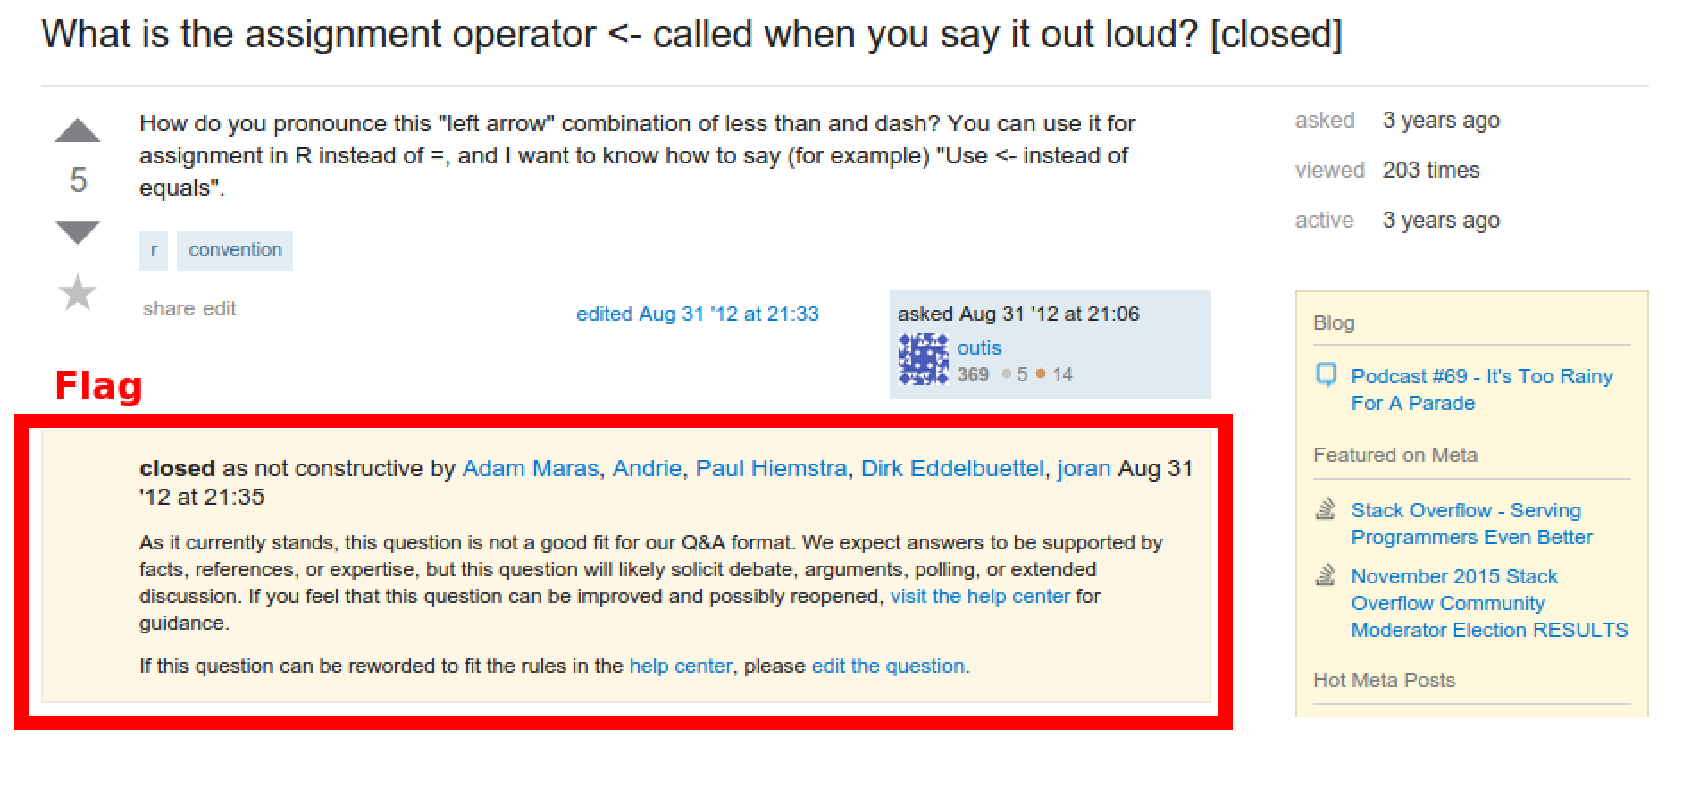
\includegraphics[width=0.9\columnwidth]{Figures/SOFlagsExample}
		\caption{Flagged post on Stack Overflow}
		\label{fig:SOFlagsExample}
	\end{figure}

	% <<UPDATED 08-12-2015 BEGIN
	On the R-help mailing list, the flag concept does not exist. 
	However, based on the definition of flags on Stack Overflow, I defined flags as messages used to call the attention of other community members.
	Based on the previous definition, flags on the R-help mailing list are used to keep a healthy community, promote discussion, and call the attention of community members to certain issues.
	In contrast with Stack Overflow, flags might be used by the person who asked or answered a question.
	Due to the plain text format of messages on the R-help mailing list, flags can be mixed among the text of answers, comments, questions and updates.
	Flags in the R-help mailing list do not constrain users to answer questions, or to clarify what it is already asked.
	% END>>

	Our analysis showed that there are six types of knowledge related to \textit{flags}:
	\begin{enumerate}[\bfseries (1)]
		\item \textbf{``Off-topic''}, \textbf{``Not constructive''} or \textbf{``opinion-based''}: They are used to identify questions that are not related to the list's interests or which answers are based on the opinion of channel participants (not actual facts).
		These flags can be assigned for different reasons or they can be used on different ways.
		\begin{itemize}
			\item \textit{Typographical error}: The problem was caused by typographical error.
			\item \textit{Debugging help}: User is asking help for debugging.
			\item \textit{Book, tool, software library}: User is asking for a book, tool, software library, tutorial or other off-site resource.
			\item \textit{Minimal understanding of the problem}: User did not demonstrate a minimal understanding of the problem being solved.
			\item \textit{Insufficient information}: the question lacks sufficient information to diagnose the problem
			\item \textit{Extra information}: User provide extra information that is not related with the questions but that it might be interesting for the user who asked the question.
			\item \textit{Homework}: When users ask something that looks like an assignment.
		\end{itemize}
		\item \textbf{``Not an answer''}: It is used to emphasize \textit{alternative answers} that are outside of the scope of the question, or to identify that a specific solution that does not answer the question.
		\item The \textbf{``Repeated question''} flag is used to acknowledge that the user is asking a repeated question. For example, because they could not find a proper answer that fit their needs, or because people did not search the archives to see if the question had already been asked.
		\item The \textbf{``Too localized''} flag is used for questions that are too specific and do not help any future reader.
		\item \textbf{``Unclear''} and  \textbf{``Not a real question''} flags are for questions that are difficult to understand.
	\end{enumerate}

%	Table \ref{table:flags} shows examples from each channel for every type of knowledge shared through flags.
%	Some flags and sub-categories are specifically of one of the channel, to the best of our knowledge, there is no example available.
%	It is worth mentioning that there are \textit{temporary flags}, and therefore, flags in one channel might not longer exist in our data.
%	For instance, in Stack Overflow an \textit{offensive} flag expires after 48 hours, which explains why there are no examples under the type \textit{rude or abusive behaviour} in Table \ref{table:flags}.

%	\begin{footnotesize}
%		\begin{longtable}{|p{4cm}|p{10cm}|}
%			\caption[Examples of flags from both channels by type of knowledge.]{Examples of flags from both channels by type of knowledge.}
%			\label{table:flags}

%			\tabularnewline
%			\hline \textbf{Type} & \textbf{Stack Overflow} \tabularnewline

%			\hline \hline \textbf{Too broad}
%			& \textit{``What tricks or functions do you use?''} {\footnotesize URL: \href{http://goo.gl/yZtDb0}{Q32888757}}\tabularnewline

%			\hline \textbf{Duplicate}
%			& \textit{``Possible duplicate of \href{http://goo.gl/yZtDb0}{Reading multiple files into R - Best practice}''} {\footnotesize URL: \href{http://goo.gl/dVhVVi}{Q32900021}}\tabularnewline

%			\hline \textbf{Unclear}
%			& \textbf{Not a real question}: \textit{``Is there any R package (or C++) that has sieve bootstrap? (The bootstrap is a method for estimating the distribution of an estimator or test statistic by resampling one’s data or a model estimated from the data...''} {\footnotesize URL: \href{http://goo.gl/FJYGgP}{Q12207195}}

%			\textbf{Unclear}: \textit{``I have a text file in the following format and I wish to extract certain lines using R. read.table("") also does not seem to work [code]''} {\footnotesize URL: \href{http://goo.gl/BeJk43}{Q12070554}}\tabularnewline

%			\hline \textbf{Off-topic}
%			& \textbf{Typographical error}: \textit{``Missing closing quotes after 9 in states''} {\footnotesize URL: \href{http://goo.gl/jDTp1W}{Q32918405}}

%			\textbf{Debugging help}: \textit{``But this code is not working. Any hints would be appreciated.''} {\footnotesize URL: \href{http://goo.gl/upGDG8}{Q32903807}}

%			\textbf{Book, tool, software library}:
%			\textit{``I want to view the R source code with any comments included, to see how the author of the package is running his code...''} {\footnotesize URL: \href{http://goo.gl/Kz9bGH}{Q18005488}}

%			\textbf{Not constructive}: \textit{``How do you pronounce this "left arrow" combination of less than and dash?...''} {\footnotesize URL: \href{http://goo.gl/8X7JAv}{Q12222481}}

%			\textbf{Minimal understanding of the problem}: \textit{``It may sound trivial in this example, but it's not in my sample. for the computation of the means, sds ect...''} {\footnotesize URL: \href{http://goo.gl/sx922W}{Q18028285}}

%			\textbf{Insufficient information}: \textit{``I'm a beginner in r programming and I'm trying to sample 25 cells all of them separated by a minimum distance...''} {\footnotesize URL: \href{http://goo.gl/UU3nEN}{Q18067248}} \tabularnewline

%			\hline \textbf{Repeated question}
%			& \textit{``This question has been asked before and already has an answer. If those answers do not fully address your question...''}  {\footnotesize URL: \href{http://goo.gl/rGtuoY}{Q15301476}} \tabularnewline

%			\hline \textbf{Too localized}
%			& \textit{``I have a folder of 100 CSV files. Each CSV file has same variables over same time period. My instructor has asked me to write a R script that will allow me to read each file to a separate Dataframe, and then call each Dataframe in R console, to get the summary statistics of the data...''}  {\footnotesize URL: \href{http://goo.gl/1wUBpH}{Q14253317}} \tabularnewline

%			%%------- R-HELP
%			\hline \hline \textbf{Type} & \textbf{R-help} \tabularnewline

%			\hline \hline \textbf{Rude or abusive behaviour}
%			& \textit{``...next time you decide to answer my question with ``RTFM'', please also include the number of the page that answers my specific question.''} {\footnotesize URL: \href{http://goo.gl/1MupSk}{Q1MupSk}}\tabularnewline

%			\hline \textbf{Not an answer}
%			& \textbf{Alternative solution}: \textit{``This is not an answer to your question, but I have used SparseM package to represent large travel time matrices efficiently... if the traveltime matrix is symmetric.''} {\footnotesize URL: \href{http://goo.gl/nnUxbM}{QnnUxbM}};

%			\textbf{Not an answer}: \textit{``Thank you very much for pointing me to meta-analysis. Although it	may not solve my problem with the normalization''} {\footnotesize URL: \href{https://goo.gl/xfTDgx}{QxfTDgx}} \tabularnewline

%			\hline \textbf{Too broad}
%			& \textit{``Your request seems too broad to allow a more focused response. Perhaps we could be more helpful if you told us what you are trying to accomplish.''} {\footnotesize URL: \href{http://goo.gl/kDYuwL}{QkDYuwL}}\tabularnewline

%			\hline \textbf{SPAM}
%			& \textit{``SPAM?''} {\footnotesize URL: \href{http://goo.gl/UHjz4f}{QUHjz4f}}\tabularnewline

%			\hline \textbf{Off-topic}
%			& \textbf{Off-topic} \textit{``The main questions here are not R-related, but statistical modeling questions, and much too broad for the R list.''} {\footnotesize URL: \href{http://goo.gl/3AGaEi}{Q3AGaEi}}

%			\textbf{Extra information}: \textit{``N.B. Off topic. This is an incredibly nice feature of R. SAS overparameterizes the design matrix and employs the sweep algorithm to zero out redundant parameters.''} {\footnotesize URL: \href{http://goo.gl/IpGVMq}{QIpGVMq}}

%			\textbf{Homework}: \textit{``This is not a homework help-line...''} {\footnotesize URL: \href{http://goo.gl/KMYykN}{QKMYykN}}
%			\tabularnewline

%			\hline \textbf{Repeated question}
%			& \textit{``I'm very sorry for my repeated question, which i asked 2 weeks ago, namely:''} {\footnotesize URL: \href{https://goo.gl/Gbek3R}{QGbek3R}}\tabularnewline
%			\hline
%		\end{longtable}
%	\end{footnotesize}

\subsubsection*{Comments}
	% <<UPDATED 08-12-2015 BEGIN
	Stack Overflow defines comments\footnote{\url{http://stackoverflow.com/help/privileges/comment}} as \textit{``...temporary `Post-It' notes left on a question or answer..''}.
	Comments can be visualized in a specific section below each question or answer.
	On Stack Overflow, comments can be used as a follow-up to questions, to answer a question, or to clarify a question.

	On the R-help mailing list, I defined comments as messages written to \emph{improve an answer in response to an incomplete question, or as follow-up on a discussion}.
	Most importantly, messages should be written by a \emph{different person than the author of the question or answer} to which they are responding.
	The difference between an update and a comment on the R-help mailing list is the motivation of the user who wrote the message and the author of the message.
	For example, if user A posts a question, B asks A to clarify something about the question, and A answers back to B, then the last message is an update and the message sent by B to A is a comment (see Figure \ref{fig:ExCommentUpdate1} top). 
	Similarly, if user A posts a question, B answers A's question, A asks B to clarify something about the answer, and B answers back to A, then the second message is an answer, the third message is a comment, and the last message is an update (see Figure \ref{fig:ExCommentUpdate1} bottom).
	% END>>

	\begin{figure}
		\centering
		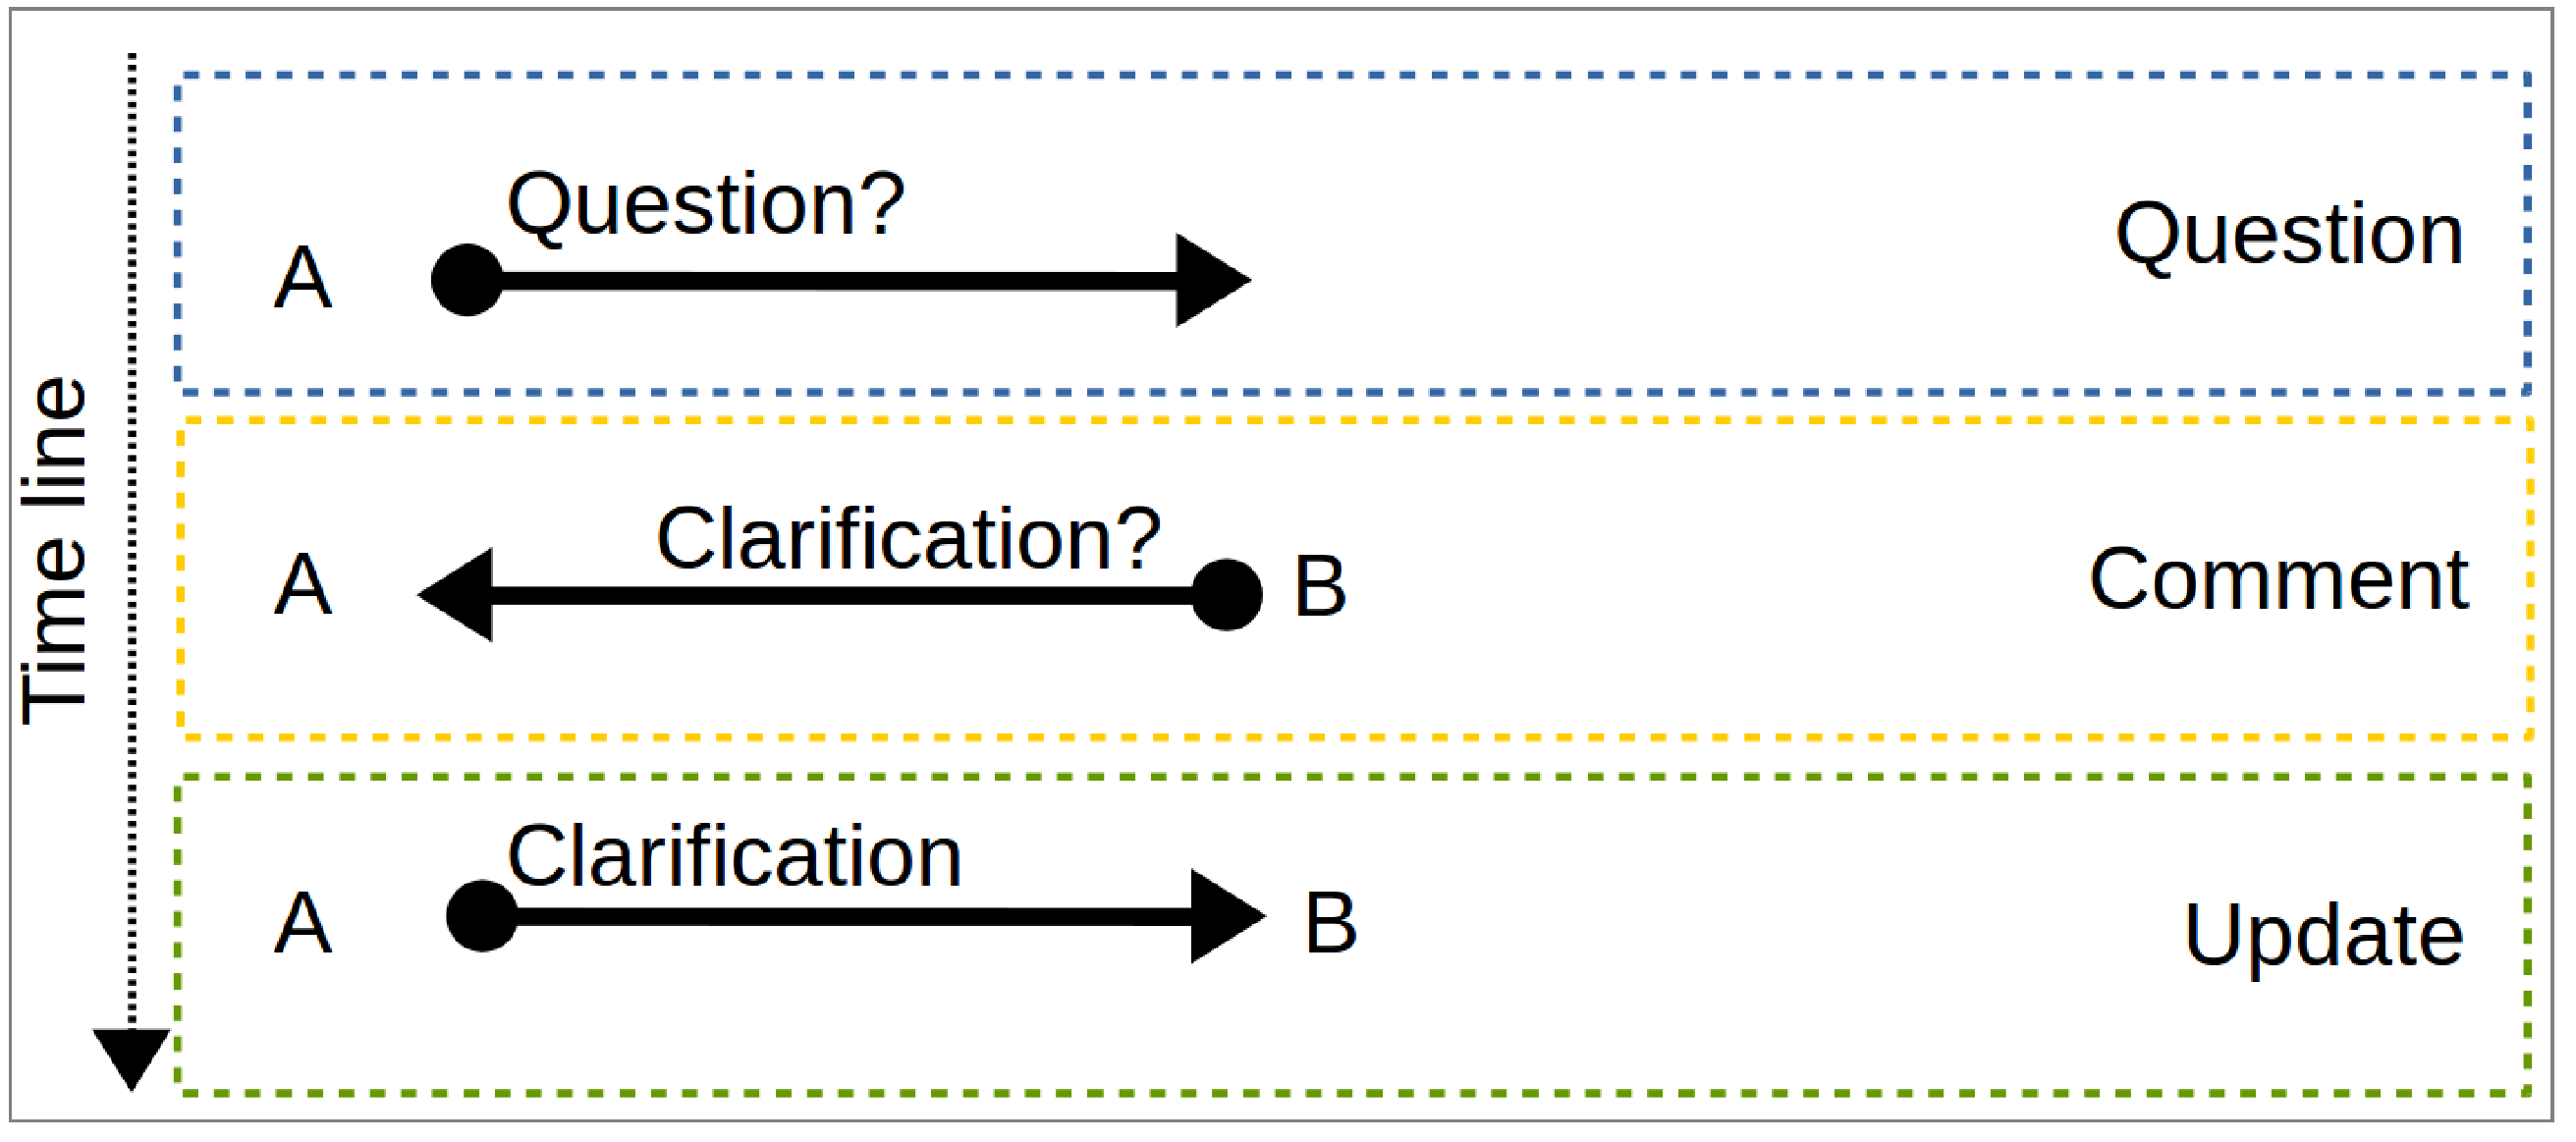
\includegraphics[width=0.7\columnwidth]{Figures/ExCommentUpdate1}
		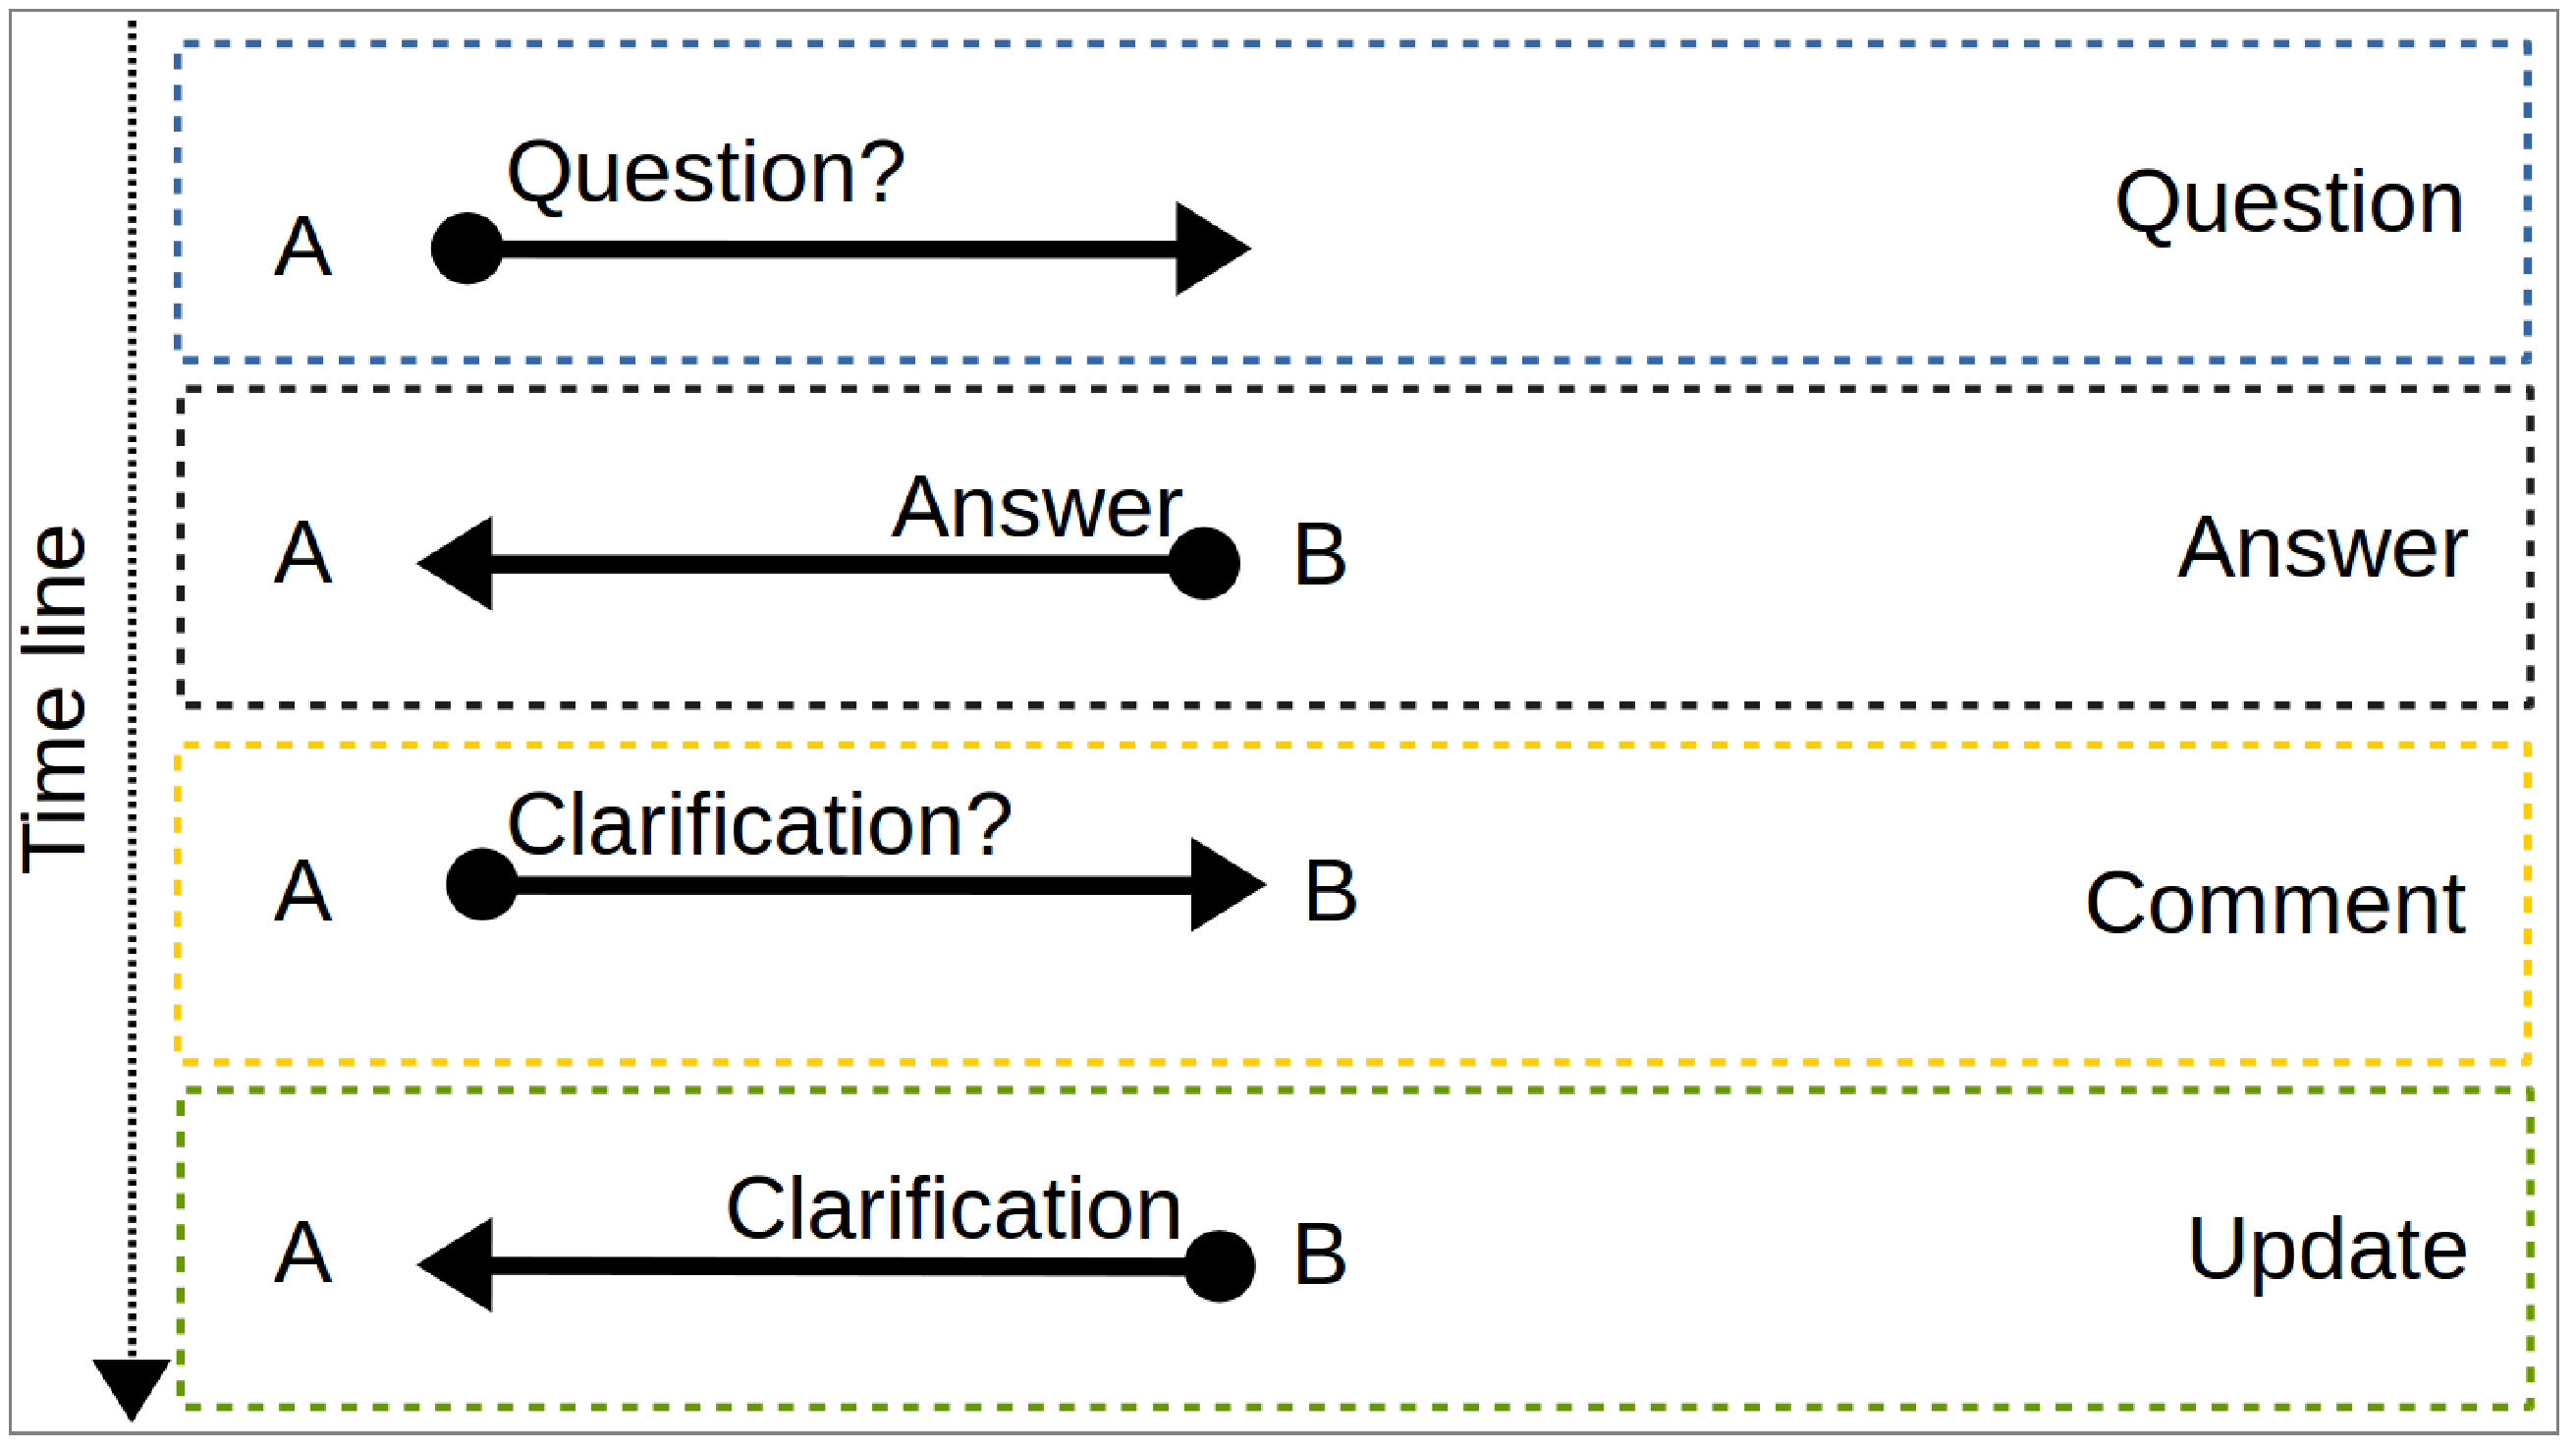
\includegraphics[width=0.7\columnwidth]{Figures/ExCommentUpdate2}
		\caption{The arrows represent a message sent to the mailing list, and the labels specify the motivation behind the message. \emph{Example 1 (Top)}: a user A posts a question; later, B asks to A to clarify something about the question; and A answers back to B. \emph{Example 2 (bottom)}: a user A posts a questions; later, B answers A's question; A asks to B to clarify something about the answer; and B answers back to A.}
		\label{fig:ExCommentUpdate1}
	\end{figure}

	Our analysis showed that there are five types of knowledge related to \textit{comments}:
	\begin{enumerate}[\bfseries (1)]
		\item \textbf{Clarification/Related question:} Provides (or requests) additional information about a question or answer.
		\item \textbf{Expansion:} Provides additional information.
		\item \textbf{Correction/Solution/alternative:} Suggests a change to a question or an answer, offers an alternative solution or a correction.
		\item \textbf{Compliment/confirmation/Criticism:} Posts something good, offers thanks, provides an opinion or criticise someone.
		\item \textbf{External reference:} References an external resource.
	\end{enumerate}

%	Table \ref{table:comments} shows examples of comments posted on each channel.

%	\begin{footnotesize}
%		\begin{longtable}{|p{3.9cm}|p{5cm}|p{5cm}|}
%			\caption{Examples of comments from both channels by type.}
%			\label{table:comments}
%			\tabularnewline
%			\hline \textbf{Type} & \textbf{Stack Overflow} & \textbf{R-help} \tabularnewline

%			\hline \hline \textbf{Clarification / Related question}
%			& \textit{``I'm not sure what that means... $>\_>$''} {\footnotesize URL:  \href{http://goo.gl/EuokIK}{Q1497539}} or \textit{``... are you aware of any coding style guidelines similar to the Python PEP?...''} {\footnotesize URL: \href{http://goo.gl/Sa8JsL}{Q1266279}}
%			& \textit{``What ``initial result''?''} {\footnotesize URL:  \href{http://goo.gl/yFlTUV}{QyFlTUV}} or \textit{``...I will actually be installing on a VM on top of an Intel box. Does that change things?...''} {\footnotesize URL: \href{http://goo.gl/5ksQUp}{Q5ksQUp}} \tabularnewline

%			\hline \textbf{Expansion}
%			& \textit{``Character vectors are supported in HDF5''} {\footnotesize URL: \href{http://goo.gl/yQA7lU}{Q7838027}}
%			& \textit{``Just to follow up on Ted's comments.... for other points in polygon algorithms. Eric Haines has made some performance evaluation of the methods... ''} {\footnotesize URL: \href{http://goo.gl/kHlQa6}{QkHlQa6}} \tabularnewline % overlap with updates

%			\hline \textbf{Correction / Alternative / Solution}
%			& \textit{``...2 simplifications: since you already are using within, there's no need to use theTable\$Position, and you could just do sort(-table(...)) for decreasing order.''} {\footnotesize URL: \href{http://goo.gl/vxPa1q}{Q5208679}}
%			& \textit{``> You seem confused. Not particularly, but he needs to be aware of \_which\_ shell R is executing in system() calls. These things work for me:''} {\footnotesize URL: \href{http://goo.gl/bdbs2x}{Qbdbs2x}}
%			\tabularnewline

%			\hline \textbf{Compliment / confirmation / Criticism}
%			& \textit{``Agreed, I'm making substantial use of 'sqldf'...''} {\footnotesize URL: \href{http://goo.gl/8wNNXy}{Q11784115}} or \textit{``+1 because those packages are great for analyzing dataframes...''}
%			{\footnotesize URL: \href{http://goo.gl/rrChQM}{Q3375808}}
%			& \textit{``Thanks ray, I really appreciate your concern...''} {\footnotesize URL: \href{http://goo.gl/kHlQa6}{QkHlQa6}}\tabularnewline

%			\hline \textbf{External reference}
%			& \textit{``See also \href{http://stackoverflow.com/q/6874867}{[here]} and \href{http://stackoverflow.com/q/2769510}{[here]}. The \href{http://www.burns-stat.com/pages/Tutor/R_inferno.pdf}{R Inferno} is also another great read.''} {\footnotesize URL: \href{http://goo.gl/X9JcRV}{Q9508518}}
%			& \textit{``I think this paper elucidates the problem Bert mentioned... \href{http://www.stat.uiowa.edu/files/stat/techrep/tr378.pdf}{paper}...''} {\footnotesize URL: \href{http://goo.gl/kHlQa6}{QkHlQa6}} \tabularnewline
%			\hline
%		\end{longtable}
%	\end{footnotesize}

	%<<
	The format of the message in Stack Overflow and the R-help mailing list, permits participants to ask multiple questions in the same thread.
	Therefore, the categorization of knowledge presented in this chapter is non-mutually exclusive. 
	%>>

\subsection{RQ-2. How is knowledge constructed on Stack Overflow and the R-help mailing list?}
\label{sec:rq2}
%\section{Construction of Knowledge}

	%[Chapter Methodology] 	We wondered if this applied to the creation and sharing of knowledge in these two channels. Our goal was to identify the mechanisms and strategies on Stack Overflow and the R-help mailing list used to construct knowledge collaboratively and individually (if any).

	Through our analysis of Stack Overflow and the R-help mailing list threads, I identified two different approaches to constructing knowledge:
	\begin{itemize}
		\item \textbf{Participatory knowledge construction} refers to answers that are created based on the cooperation of multiple users in the same thread.
		Participants complement each other's questions by providing pros and cons about the answer, different viewpoints, or additional context and examples.
		Participatory knowledge is comparable with the team concept in which people work together in a cooperative way for the same objective.

		\item \textbf{Crowd knowledge construction} leverages the experiences of many users; it allows them to contribute their individual explanations and practices adding variety to the pool of solutions.
		Crowd knowledge is comparable with the group concept in which people work towards the same objective but not necessarily together. Participant can vote over others ideas, but the idea is not constructed through a discussion process.
	\end{itemize}

	On the R-help mailing list, participatory knowledge takes place when:
	(1) previous answers are included in the actual answer and it is possible to infer a link between them; or
	(2) when a direct reference to other answers or authors is expressed in the message.
	Figure \ref{fig:ML-PK1} depicts two examples of the way participatory knowledge occurs on the R-help mailing list:
	direct citation of the author of a previous answer (top), and inferable links between answers (right).

	
	\begin{figure}[!htb]
		\centering
		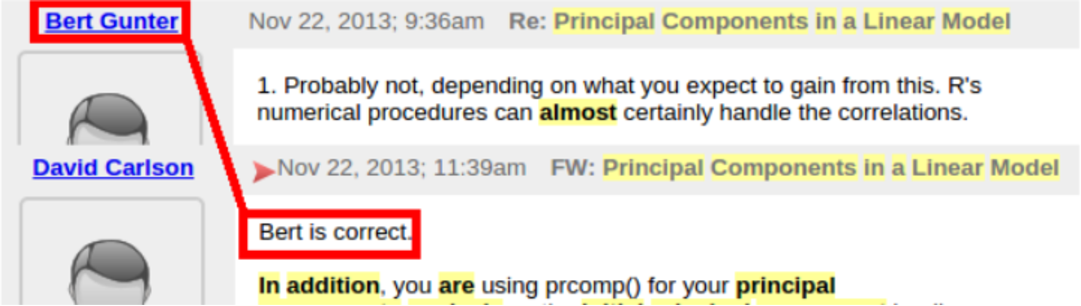
\includegraphics[width=0.8\columnwidth]{Figures/ML-PKimg2}
		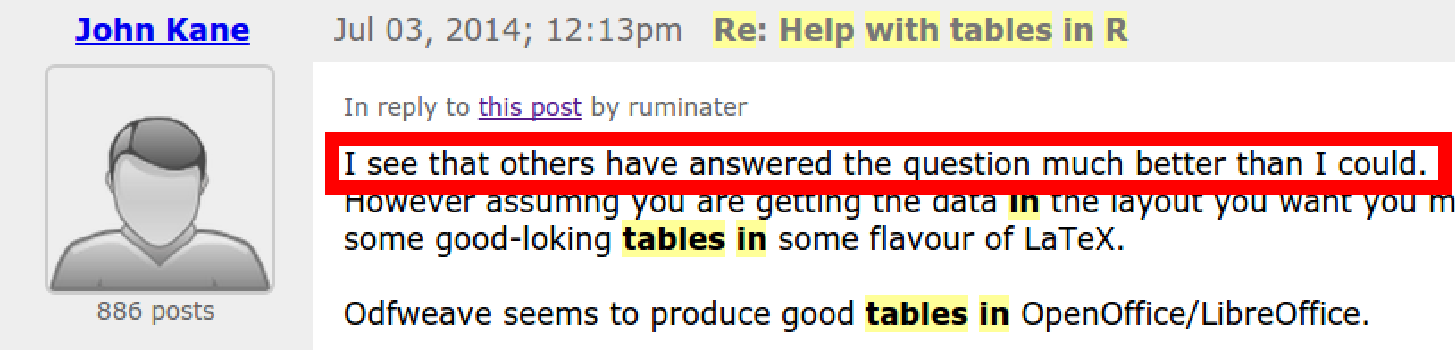
\includegraphics[width=0.8\columnwidth]{Figures/ML-PKimg11}
		\caption[Participatory knowledge on the R-help mailing list.]{Participatory knowledge on the R-help mailing list.}
		\label{fig:ML-PK1}
	\end{figure}

	On Stack Overflow, participatory knowledge takes place when:
	(1) it is possible to infer a link between answers (i.e., direct or indirect reference); or
	(2) comments complement the answer, or directly cite another author.

	On Stack Overflow, participatory knowledge happens in different places, perhaps as a consequence of its rich interface.
	We see this, when a user answers a question and directly cites or links to the author of another answer in the thread, or when a user cites the author of a question or answer in a comment made on that question or answer, by including more information or by suggesting that the answer provided is an additional solution.
	Figure \ref{fig:SO-PK1} depicts four examples where participatory knowledge occurs in Stack Overflow: one answer references the author of another answer (top left); the comments expand the answer (top right); the comments reference another answer for a specific scenario (bottom left); and an inferable link between the actual answer and a previous one (bottom right).

	\begin{figure}[!htb]
		\centering
		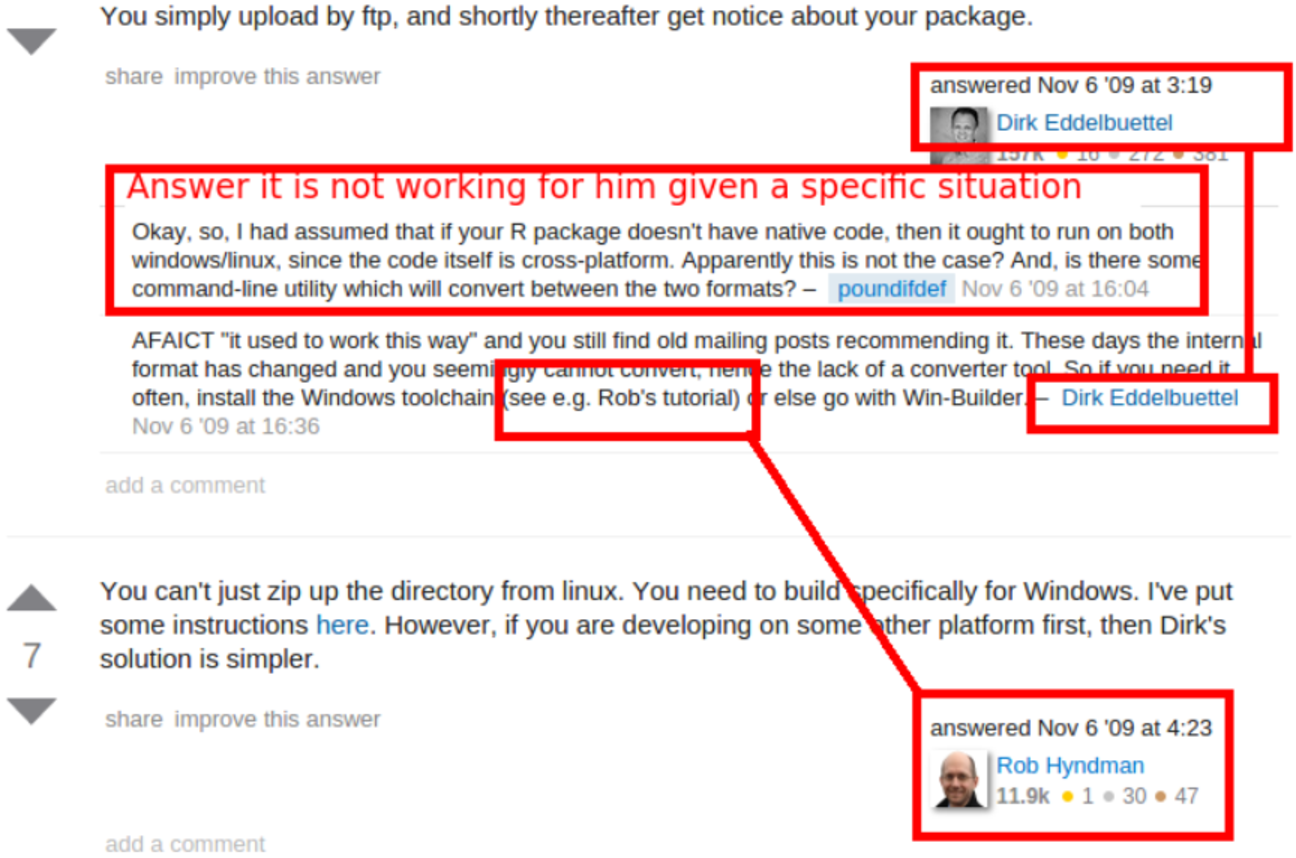
\includegraphics[width=.8\columnwidth]{Figures/SO-PKimg5}
		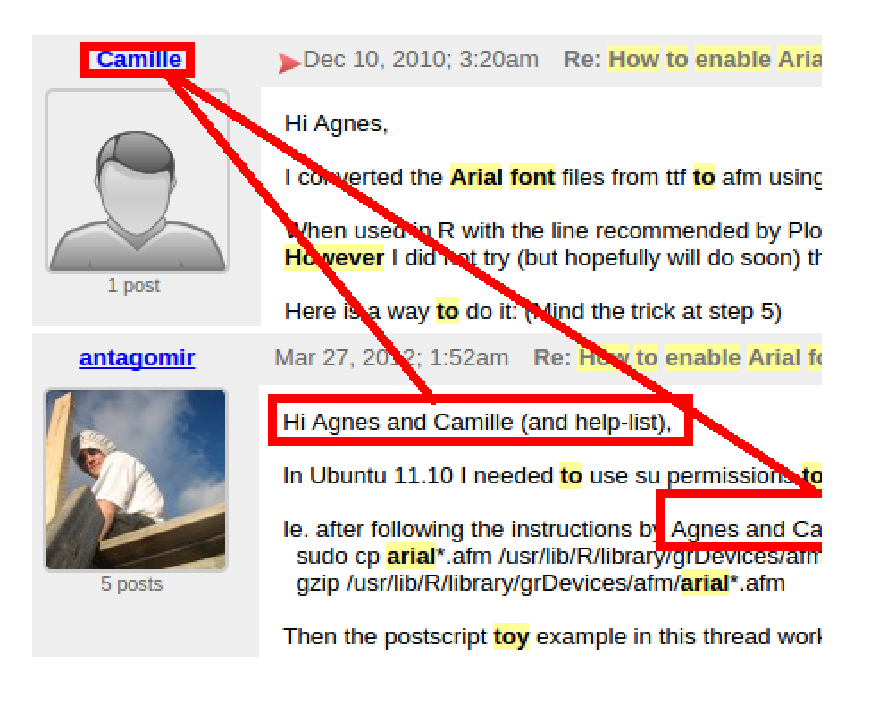
\includegraphics[width=.8\columnwidth]{Figures/ML-PKimg1}
		\caption{Participatory knowledge on Stack Overflow.}
		\label{fig:SO-PK1}
	\end{figure}

	Crowd knowledge construction is observable when: 1. There is not a direct or inferable reference between answers, 2. Answers are a variation of one of the answers on the thread.
	Figure \ref{fig:CKC_MLSO} depict an example of how crowd knowledge construction is visible on Stack Overflow.
	As can be seen from the figure, there are two of the three answers that provided a repeated solution.

%	\remarks{FIX THE FIGURE}

	\begin{figure} [!htb]
		\centering
		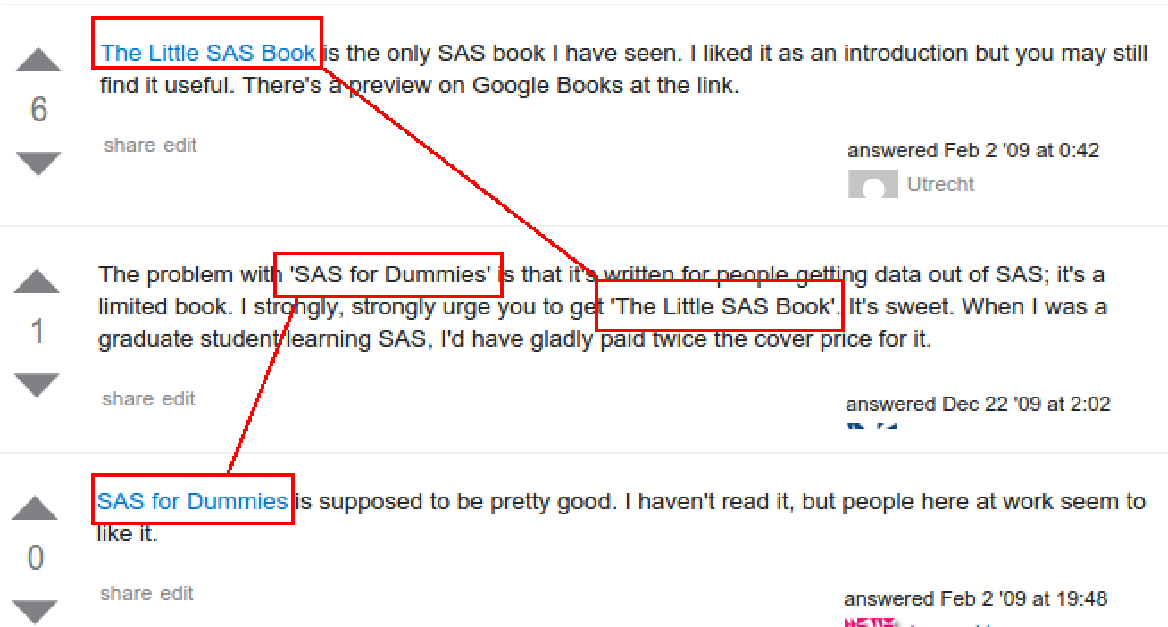
\includegraphics[width=0.8\columnwidth]{Figures/SO-CSimg2}
		\caption{Examples of how crowd knowledge construction occurs.}
		\label{fig:CKC_MLSO}
	\end{figure}

\subsection{RQ-3. How does the sharing of links on Stack Overflow and the R-help mailing list support knowledge construction? }
%\section{External Resources and the Construction of Knowledge}

	% [Chapter Methodology]	We wondered if this was also true for the R-help mailing list. More importantly, we wanted to know how this network of links contributes to the construction of knowledge.

	External resources contain information that is valuable for questions and answers.
	More importantly, they contribute to the construction of knowledge, often by simplifying answers and other contributions.
	However, depending on the type of resource (e.g., forum, Q\&A Website, or Wiki), the support might be different.
	% <<UPDATED 08-12-2015 BEGIN
	We found that each type of resource is shared and supports knowledge on Stack Overflow and the R-help mailing list in the same way.
	% END>>

	Our analysis showed that there are 11 resource types:
	\begin{enumerate}[\bfseries (1)]
		\item \textbf{Q\&A channels}: A online media channels for asking questions and answers (e.g., Stack Overflow and the R-help mailing list).
		\item \textbf{Source code management systems, project hosting or issue trackers}: Online services that provided support for management of changes to documents (e.g., GitHub), hosting of projects (e.g., SourceForge or Google Code), and management of the software issues (e.g., Bugzilla).
		\item \textbf{File hosting}: Online services that provide support for management of files (e.g., MediaFire and Dropbox).
		\item \textbf{Digital Libraries, papers, books and journals}: Online services that provide access to papers, books, journals (e.g., R Journal arXiv).
		\item \textbf{Forums}: Online discussion website where people can hold conversations in the form of posted messages (e.g., Google Groups).
		\item \textbf{Wiki}: Online website that allows collaborative modification of its content through the web browser (e.g., Wikipedia).
		\item \textbf{Blog}: An informal website to published discussion, ideas, and tutorial (e.g., Wordpress).
		\item \textbf{Official documentation}: Documentation published by the original source of the technology (e.g., CRAN)
		\item \textbf{Libraries, packages and applications}: collection of non-volatile source code or resources used by programs (e.g., GGPLOT) or entire software solutions (e.g., RSTudio)
		\item \textbf{Online environments}: website that provide online environments such as IDE or notepads with source code syntax highlighting (e.g., GitHub Gits, or Pastebin)
		\item \textbf{Other}: Websites from companies, non- official documentation sites, or any other online services do not include on the previous resources list.
	\end{enumerate}

	Additionally, we identified 10 types of resources that are linked to support knowledge construction:
	\begin{enumerate}[\bfseries (1)]
		\item \textbf{Answers}: Links to an answer on a Q\&A media channel.
		\item \textbf{Tutorial/Guide}: Links to tutorial or guides.
		\item \textbf{Source code/Examples}: Links to source code example, implementation, or final products.
		\item \textbf{Channel}: Link to a an specific media channel.
		\item \textbf{Expand/Background}: Links to a source of information that should be read.
		\item \textbf{Books and papers}: Links to books, papers, and journals
		\item \textbf{Hacks}: Links to workarounds.
		\item \textbf{Images}: Links to images.
		\item \textbf{Data}: Links to data.
		\item \textbf{Announcement}: Links to company or personal webpage or project.
	\end{enumerate}

%	Table \ref{table:motiveType} summarizes the types of external resources my colleague and I found in our study and the ways these resources support the construction of knowledge.

%	\begin{footnotesize}
%		\begin{longtable}{|p{4cm}|p{10cm}|}
%			\caption{External resources and the construction of knowledge.}
%			\label{table:motiveType}
%			\tabularnewline
%			\hline \textbf{Resource Type} & \textbf{Ways to Support Knowledge}\tabularnewline
%			%%%%%
%			\hline \hline \textbf{Q\&A channels}
%			& \textbf{Answer}: \textit{``...Here's the salient Python code you can retrofit into your calls in rJython, borrowing directly from \href{http://mg.pov.lt/blog/unicode-emails-in-python}{the aforementioned blog post}: [code]...''} {\footnotesize URL:  \href{http://goo.gl/d2FNDo}{Q10027560}}

%			%Steps that have been followed
%			\textbf{Tutorial / Guide}: \textit{``As a end note, I read \href{http://stackoverflow.com/questions/5963269/how-to-make-a-great-r-reproducible-example}{How to make a great R reproducible example?} and tried my best''} {\footnotesize URL:  \href{http://goo.gl/XU1iLco}{Q5963269}}

%			\textbf{Channel}: \textit{``...If you have questions about xcode, ..., then a better place might be the r-sig-mac mailing list: \href{https://stat.ethz.ch/mailman/listinfo/r-sig-mac}{[here]}...''} {\footnotesize URL:  \href{http://goo.gl/YByST9}{QYByST9}}

%			\textbf{Source code/Examples}: \textit{``The following function (found \href{http://r.789695.n4.nabble.com/Email-out-of-R-code-td3530671.html\#a3948061}{here}) works well for messages containing ASCII characters...''} {\footnotesize URL:  \href{http://goo.gl/Ow1da5}{Q10027560}}
%			\tabularnewline

%			\hline \textbf{Source code management systems, project hosting or issue trackers}
%			& \textbf{Answer}: \textit{``Look into Sweave or knitr to combine R and LaTeX for producing reports. hth, Ingmar \href{http://www.statistik.lmu.de/~leisch/Sweave/}{[Sweave]} \href{https://github.com/yihui/knitr}{[knitr]}''} {\footnotesize URL:  \href{http://goo.gl/vJEJlU}{QvJEJlU}}

%			\textbf{Expand / Background}: \textit{``All I can suggest in this case is to update R and run update.packages() as indicated by FAQ1: \href{https://github.com/yihui/knitr/blob/master/FAQ.md}{[here]}''} {\footnotesize URL:  \href{http://goo.gl/d2rylY}{Qd2rylY}}

%			\textbf{Tutorial/Guide}: \textit{``...This way is taken from this rCharts 'official' \href{http://ramnathv.github.io/rCharts/}{tutorial} (find m1 plot code)...''}  {\footnotesize URL:  \href{http://goo.gl/SWVCpm}{Q19339766}}

%			\textbf{Books and papers}: \textit{``If you are still unable to find it, please go to: \href{https://github.com/downloads/yihui/lyx/sweave.pdf}{[LaTeX document on GitHub]} It is a compiled version of the manual. ''} {\footnotesize URL:  \href{http://goo.gl/q6b1Rr}{Qq6b1Rr}}

%			\textbf{Hacks}: \textit{``...As per mentioned by @GeorgeDontas in the comments, there is a little hack \href{https://github.com/rich-iannone/DiagrammeR/issues/77}{[Issue on GitHub]} that could allow to change the labels of the x axis to dates instead of 'w.01, w.02'...''} {\footnotesize URL:  \href{http://goo.gl/LJzWS6}{QLJzWS6}}
%			\tabularnewline

%			\hline \textbf{File hosting}
%			& \textbf{Images}: \textit{``I'm trying to plot some data over a background image. The problem is that both layers end up using the same scale. This is unfortunately problematic. An example.			I want to plot some data over this \href{https://dl.dropboxusercontent.com/u/39251/image.jpg}{image} ... Plotting the sample data, I get \href{https://dl.dropboxusercontent.com/u/39251/data.png}{this}...''}  {\footnotesize URL:  \href{http://goo.gl/XJzOi6}{Q16409935}}

%			\textbf{Source code / Examples}: \textit{``...I am doing sentiment analysis using score.sentiment... from the below link you can see how this work... \href{http://dl.dropbox.com/u/2698672/sentiment.r}{[r-file on dropbox]}...''} {\footnotesize URL:  \href{http://goo.gl/9g8UPi}{Q9g8UPi}}

%			\textbf{Data}: \textit{``I have weekly sales observations for several products drawn via ODBC. Source data is available at \href{https://www.dropbox.com/s/78vxae5ic8tnutf/asr.csv}{[here]} ''} {\footnotesize URL:  \href{http://goo.gl/tMpK31}{QtMpK31}}
%			\tabularnewline

%			\hline \textbf{Digital Libraries, papers, books and journals}
%			& \textbf{Tutorial / Guide}: \textit{``You can reduce the text size using the "grid.gedit" approach described at the end of the ggplot book, available on Hadley Wickham's website:
%			\href{http://had.co.nz/ggplot2/book.pdf}{[ggplot book]}''} {\footnotesize URL:  \href{http://goo.gl/xho3GJ}{Qxho3GJ}}

%			\textbf{Source code / Examples}: \textit{``...Meanwhile, I would like to point out that any of these linear restrictions can be reformulated as an exclusion restriction, see for example the remark on pages 5-6 of \href{http://www.econ.uiuc.edu/~roger/research/ranks/ranktests.pdf}{[Gutenbrunner et al. paper]} or the references cited there.  And using this sort of parametrization you can use anova.rq()...''} {\footnotesize URL:  \href{http://goo.gl/Z7OYEm}{QZ7OYEm}}

%			\textbf{Expand/Background}: \textit{``...I started by reading through \href{http://cran.r-project.org/doc/contrib/Ricci-distributions-en.pdf}{[Ricci distribution manual]}... ''} {\footnotesize URL:  \href{http://goo.gl/M21jAN}{QM21jAN}} or \textbf{Expand}: \textit{``I suspect you are trying to find your way into Circle 6 of 'The R Inferno' but haven't yet got in. \href{http://www.burns-stat.com/pages/Tutor/R\_inferno.pdf}{[R Inferno]}''} {\footnotesize URL:  \href{http://goo.gl/xF1j3R}{QxF1j3R}}
%			\tabularnewline

%			\hline \textbf{Forums}
%			& \textbf{Expand / Background}: \textit{``...to include the raw HTML in my page but I receive a 404 error with these as well as when I attempted to include it as an iframe within R-Shiny (following this \href{https://groups.google.com/forum/\#!msg/shiny-discuss/wcL9HE15rtk/3ipbwiR75D4J}{[Discussion Google Groups]})...''} {\footnotesize URL:  \href{http://goo.gl/BHymWY}{Q23618813}}

%			\textbf{Tutorial / Guide}: \textit{``Success. For myself and FWIW to other useR's here's how i spent the sunny half of my sunday to achieve it :/... \#\# Per- \href{http://ubuntuforums.org/showthread.php?t=1491846}{[ubuntuforums]}''} {\footnotesize URL:  \href{http://goo.gl/7cpqVb}{Q7cpqVb}}

%			\textbf{Source code / Examples}: \textit{``...this might be what you need (the following example is taken from \href{http://www.lispforum.com/viewtopic.php?f=2\&t=386}{[lispforum]})...''} {\footnotesize URL:  \href{http://goo.gl/Yhjxrq}{Q3300900}}

%			\textbf{Channel}: \textit{``There is a separate ggplot2 mailing list at \href{https://groups.google.com/forum/\#!forum/ggplot2}{[ggplot forum]}, please post future ggplot2 questions there.''} {\footnotesize URL:  \href{http://goo.gl/0c7ypZ}{Q0c7ypZ}}

%			\textbf{Answer}: \textit{``...If you're looking to improve the approach itself, \href{http://mathforum.org/library/drmath/view/54367.html}{[see here]}...''} {\footnotesize URL:  \href{http://goo.gl/duC1EB}{Q3137168}}
%			\tabularnewline

%			\hline \textbf{Wiki}
%			& \textbf{Expand / Background}: \textit{``...how to properly \href{https://en.wikipedia.org/wiki/Unicode\_and\_email}{[send Unicode email]}, which you're using Python to manage the underling SMTP connection for...''} {\footnotesize URL:  \href{http://goo.gl/d2FNDo}{Q10027560}}
%			\tabularnewline

%			\hline \textbf{Blog}
%			& \textbf{Expand / Background}: \textit{``...Slightly on topic, just yesterday, the CFPB announced they'll be using R in their work: \href{http://blog.revolutionanalytics.com/applications/}{[Instrumental Variables]}...''} {\footnotesize URL:  \href{http://goo.gl/kvyDvZ}{QkvyDvZ}}

%			\textbf{Tutorial / Guide}: \textit{``Saving full environments is possible, but it is very easy to start loosing track on where each variable came from. You might want to use this process: \href{http://www.r-bloggers.com/a-better-way-of-saving-and-loading-objects-in-r/}{[here]}''} {\footnotesize URL:  \href{http://goo.gl/NWMm2w}{QNWMm2w}}

%			\textbf{Answer}: \textit{``you can see the whole algorithm of sentiment analysis from the below link \href{https://dataissexy.wordpress.com/2012/02/01/twitter-sentiment-analysis-in-30-seconds/}{[here]}''}
%			{\footnotesize URL:  \href{http://goo.gl/9g8UPi}{Q9g8UPi}}
%			\tabularnewline

%			\hline \textbf{Official documentation}
%			& \textbf{Expand / Background}: \textit{``...You should be able to open a text connection using \href{http://stat.ethz.ch/R-manual/R-devel/library/base/html/connections.html}{?file} with the open argument set to write...''} {\footnotesize URL:  \href{http://goo.gl/6YfShw}{Q19601034}}

%			\textbf{Answer}: \textit{``However, you may be experiencing a problem in your PDF viewer (Preview?) due to anti-aliasing, which is noted here: \href{http://cran.r-project.org/doc/FAQ/R-FAQ.html\#Why-are-there-unwanted-borders}{[link]}''} {\footnotesize URL:  \href{http://goo.gl/bESGwE}{QbESGwE}}

%			\textbf{Tutorial/Guide}: \textit{``...I am trying to grok the information \href{http://cran.r-project.org/doc/manuals/R-exts.html\#Using-Makevars}{[here]}, where it says...''} {\footnotesize URL:  \href{http://goo.gl/l2EnfL}{Ql2EnfL}}
%			\tabularnewline

%			\hline \textbf{Libraries, packages and applications}
%			& \textbf{Answer}: \textit{``RStudio IDE (Server) may be the answer to your question. Have a look at \href{http://www.rstudio.com/ide/}{[RStudio]}''} {\footnotesize URL:  \href{http://goo.gl/6q2gSV}{Q13705519}}
%			\tabularnewline

%			\hline \textbf{Online environments}
%			& \textbf{Source code / Examples}: \textit{``Here is my version of the function... \href{https://gist.github.com/low-decarie/2599463}{It is available here as a gist}...''} {\footnotesize URL:  \href{http://goo.gl/qI7TZF}{Q10454973}}
%			\tabularnewline

%			\hline \textbf{Other}
%			& \textbf{Announcement}: \textit{``...It looks like it is what powers the awesome \href{http://www.rdocumentation.org/}{[rdocumentation.org]} site...''} {\footnotesize URL:  \href{http://goo.gl/6q2gSV}{Q13705519}}

%			\textbf{Source code / Examples}: \textit{``National Weather Service to generate graphics representing real-time hydrologic ensemble (probabilistic) forecasts. Go to: \href{http://www.erh.noaa.gov/mmefs/ }{[here]} to see. ''} {\footnotesize URL:  \href{http://goo.gl/kvyDvZ}{QkvyDvZ}}
%			\tabularnewline
%			\hline
%		\end{longtable}
%	\end{footnotesize}

\subsection{RQ-4. Why do Certain Users Post to Both Stack Overflow and the R-help Mailing List}
%\section{Characterization of the Knowledge \\from Active Users}

	For a community such as R, the variety of channels makes it possible to reach different users of the same community.
	Therefore, it is possible to find that a question is posted in both channels by the same user.
	I was motivated to understand the reasons, as well as the benefits or disadvantages of posting the same questions in both channels at the same time.

	I identified that being active on both channels at the same time brings some benefits:
	\begin{itemize}
		\item \textbf{Improve the existing answer:} If a question hasn't been answered in one channel, an answer may exist in another channel.
		\item \textbf{Support follow-up questions:} If a question is already closed and further questions arise, users can use other channels to reach out for help.
		\item \textbf{Speeds up answers:} Users can ask the same question on both channels to speed up the process, and at the same time, get more points of view. However, this behaviour is not encouraged by the community as it is deemed impolite.
	\end{itemize}

%	Table \ref{table:multiChannel} provide examples of the benefits of using both channels.

%	\begin{footnotesize}
%		\begin{longtable}{|p{5cm}|p{9cm}|}
%			\caption{Examples of the benefits of using both channels.}
%			\label{table:multiChannel}
%			\tabularnewline
%			\hline \textbf{Type} & \textbf{Description}\tabularnewline

%			\hline \hline \textbf{Improve the existing answer} %\remarks{choose another example, this one is not working anymore}
%			& \textbf{Cross-posting warning}: A user asks a question on Stack Overflow ({\footnotesize URL:  \href{http://goo.gl/k9OqUH}{Q17133550}}). A few days later, the user asks the same question on the R-help mailing list ({\footnotesize URL:  \href{http://goo.gl/hPZmXo}{QhPZmXo}}) warning readers that she posted the same question on Stack Overflow without any successful answer. Years later, the question is answered on Stack Overflow. \tabularnewline

%			\hline \textbf{Support follow-up questions}
%			& A user posts a question on the R-help mailing list {\footnotesize URL:  \href{http://goo.gl/QaUoJ3}{QQaUoJ3}} and gets some answers. However, the follow-up question is not answered on the R-help list, so the user asks the extra questions on Stack Overflow. {\footnotesize URL:  \href{http://goo.gl/nmiKhj}{Q12156939}} \tabularnewline

%			\hline \textbf{Speed up answer}
%			& \textbf{Cross-posting without warning (no one noticed the cross-posting)}: A user sent an email to the R-help mailing list ({\footnotesize URL:  \href{http://goo.gl/ZCCLj7}{QZCCLj7}}), and a few minutes later, asked the same question on Stack Overflow ({\footnotesize URL:  \href{http://goo.gl/xaB5kO}{Q12156939}}). On both channels, the community answered the question.
%			Next, the user asked a follow-up question on just the R-help mailing list, which was answered satisfactorily.

%			\textbf{Cross-posting without warning (someone noticed the cross-posting)}: A user asks a question on Stack Overflow, Cross Validate and the R-help mailing list. Someone notices it and posts back to the R-help list saying \textit{``Crossposting to CrossValidated and StackOverflow and to Rhelp is deprecated. You should offer code and data and explain why the answers you have already been given are not adequate.''} {\footnotesize URL:  \href{http://goo.gl/xW5gdw}{QxW5gdw}}
%			\tabularnewline
%			\hline
%		\end{longtable}
%	\end{footnotesize}

\subsection{User Behaviours}
\label{sec:userbeh}

	While analysing questions and answers, my colleague and I identified user behaviours that are not reflected in the categories we developed, but that I believe are worth mentioning.
	These behaviours provide evidence of their altruistic way of thinking and the strong commitment that users have within the community.
	\begin{itemize}
		\item \textbf{I answered my own question}: Some questions are answered by the same user who asked the question. They posted back to the channel to document their solution.
		(e.g., \textit{``I've discovered the answer to my own question.''} {\footnotesize URL:  \href{http://goo.gl/FG59Mw}{Q18450396}} or \textit{``Just for the records (and if anyone ever wants to find the ``solution"), I solved my own problem.''} {\footnotesize URL:  \href{https://goo.gl/r3z0DX}{Qr3z0DX}}).

		\item \textbf{I did it for you}: There are occasions when answering authors provides an extensive amount of source code to help others. For instance, \textit{``I have coded up the algorithm from the Cameron and Turner paper. Dunno if it gives exactly the same results as my (Splus?) code from lo these many years ago...''} {\footnotesize URL:  \href{http://goo.gl/GXWGG3}{QGXWGG3}}.

		\item \textbf{Answered, updated or continued years later}: Some answers are provided months or years after the question was asked.
		For instance, a user on Stack Overflow modified an answer to provide a more updated version of the source code (i.e., {\footnotesize URL:  \href{http://goo.gl/k6ZARR}{Q1724024}}); and a question asked on the R-help mailing list in 2012 was continued two years later (i.e., {\footnotesize URL:  \href{http://goo.gl/kgSHZv}{QkgSHZv}}).

		\item \textbf{Ideas for improvement or creation of the channel}: This behaviour is specific for the R-help mailing list. Sometimes users suggest modifications or new features to improve the channel. For instance a user proposes to create a package repository that can be accessible through a public wiki, or version control interface (i.e., {\footnotesize URL:  \href{http://goo.gl/p0IunD}{Qp0IunD}}).
%		There are also messages to motivate community members to generate new ideas. For instance, a user encourages the community to provide new ideas to improve a well known site for review and tag R packages (i.e.,{\footnotesize \href{http://goo.gl/63AFxN}{Q63AFxN}}).
%		Finally, a user proposes to discuss the future of the R-help mailing list given the existence of Stack Overflow ({\footnotesize URL:  \href{http://goo.gl/GtUpfb}{QGtUpfb}}).
	\end{itemize}

	I also identified two behaviours that might result in a bad response from the community:
	\begin{itemize}
		\item \textbf{Cross-posting:} The user posts the same question in both channels at the same time.
		For instance: \textit{``-1 for cross posting to r-help – [user name]''} {\footnotesize URL: \href{http://goo.gl/ENKrVK}{Q5436630}}
		\item \textbf{Posting guidelines violation:} The user behaves in such a way that it becomes apparent that they did not read the posting guidelines.
		For instance, a user asked a question that seems to be the opposite of what the posting guide recommend, and someone answered: \textit{``...If you read the Posting Guide I think you will find precisely the opposite expectation explicitly presented. Using my "cheeky code" would only be part of the recommended actions to take before posting if you follow the recommendations of the "Do your homework before posting:"...''} {\footnotesize URL: \href{http://goo.gl/FUm1HC}{QFUm1HC}}
	\end{itemize}

\subsection{Survey Results}
\label{sec:survey}

	As previously mentioned, the objective of the survey was to bring further insights on the study.
	In the survey, the main findings aligned with the thesis results come from the open questions that gather information about the experiences of the participants on Stack Overflow and the R-help mailing list.
	Given the nature of my study, I was interested in the opinions regarding the preferences of one channel over the other, as well as any challenges that the participants might have experienced.
	Tables \ref{table:surveySO} and \ref{table:surveyML} summarize the results of the following open questions (scattered among sections 2 to 4 of the survey) in terms of the pros and cons of both media channels.

	{\itshape
	\begin{itemize}
		\item Have you experienced any challenges using Stack Overflow? Please elaborate.
		\item What motivates you to answer questions or add comments on Stack Overflow? Please elaborate.
		\item Have you experienced any challenges using the R-Help Mailing List? Please elaborate.
		\item What motivates you to answer questions on the R-Help Mailing List? Please elaborate.
		\item Why do you think the R-Help Mailing List has been replaced by Stack Overflow? Please elaborate.
		\item In what situations would you choose Stack Overflow over the R-Help Mailing List? Please elaborate.
		\item In what situations would you choose the R-Help Mailing List over Stack Overflow? Please elaborate.
	\end{itemize}
	}

	These questions were intended to provide insights to understand why these channels are used, as well as some opportunities for improvement.
	Table \ref{table:surveySO} refers to the pros and cons of Stack Overflow.
	The reported benefits of using Stack Overflow were as follows: peer recognition, a friendly and rich interface, answers are straight to the point, it is easy to search for information, and questions are answered faster.
	However, the drawbacks of Stack Overflow include: strict rules become an obstacle sometimes and add complexity, the abundance of related questions, certain level of experience is required to understand the answers, and limitations on the scope of topics to discuss.

	Similarly, Table \ref{table:surveyML} refers to the pros and cons of the R-help mailing list.
	The benefits of using the R-help list include: the convenience of just handling email, the information can be used to learn, the answers are more focused, the participation of highly experienced users (i.e., rock stars), and its flexibility.
	The disadvantages that were reported include: sometimes there can be aggressive behaviour, performing search is not easy, email is not a desirable interface, and the lack of categorization given the massive volume of information.

%	\begin{footnotesize}
%		\begin{longtable}{|p{14cm}|}
%			\caption{Summary of pros and cons for Stack Overflow. The numbers between square brackets correspond to how many users support the same topic {\footnotesize (*) \textit{UX} is the participants ID for the survey where X the participant ID}}
%			\label{table:surveySO}
%			\tabularnewline
%			\hline
%			\textbf{\large Pros}
%			\tabularnewline
%			\hline
%			\hline
%			\textbf{Peer recognition}: [U3, U31] \textit{``Stack is a nice place to get peer recognition. Plus it's very nice to be able to give back to the R community.''} U3 \textbf{(*)}
%			\tabularnewline
%			\textbf{Interface}: [U14] \textit{``SO is an excellent model for providing a rich resource for users of R, which the R-Help mailing list was not. Ability to include light markup, render code blocks nicely, not have nested email threads all helps the experience of searching for and finding the help that a user needs and I want to contribute to that.''} U14
%			\tabularnewline
%			\textbf{To the point}: [U3] \textit{``...If I actually want an answer and not a lecture.''} U3
%			\tabularnewline
%			\textbf{Searchability}: [U6,U16] \textit{``SO shines when searching because of tags and ratings.''} U6
%			\tabularnewline
%			\textbf{Response time and clarity}: [U35] \textit{``I tend to prefer Stack Overflow for posting questions. The response time is often quite fast. The question and answers are preserved cleanly for the future.''} U35
%			\textbf{Learning}: [U7,U23] \textit{``If it is an area, I want to increase my proficiency in I may use it as a study device...''} U7
%			\tabularnewline
%			\tabularnewline
%			\hline	\hline
%			%			%CONS
%			\textbf{\large Cons}\tabularnewline	\hline	\hline
%			\textbf{Strict}: [U4] \textit{``I find the rules about asking confusing and very strictly monitored. I often find questions that I would love to be answered get closed for being against the rules.''} U4
%			\tabularnewline
%			\textbf{Complexity}: [U14] \textit{``Only learning the Stack Exchange Ethos of what good questions \& answers constitute and the way the system has evolved in terms of community/tag curation regarding questions (e.g. changes to close vote reasons)''} U14
%			\tabularnewline
%			\textbf{Duplicity}: [U2, U13] \textit{``Too many related questions, needs i) de-duplication ii) more maintenance to avoid duplication''} U2
%			\tabularnewline
%			\textbf{Friendliness}: [U3,U35] \textit{``If I'm feeling just a little too good about myself and I want someone on the internet to tell me what a n00b I am.''} U3
%			\tabularnewline
%			\textbf{Participants experience}: [U25, U26] \textit{``The widely varying expertise of the contributors necessitates careful consideration of some of the answers''} U25
%			\tabularnewline
%			\textbf{Ownership of the information}: [U27] \textit{``...I don't know how SO is funded, but it looks for-profit, and many R users won't support it for that reason. There's also a concern that it may shut itself down at some point, and all the postings on it will be lost. There are multiple archives of the R-help list, so that's unlikely. There can't be multiple archives of SO, because they claim copyright on the compilation.''} U27
%			\tabularnewline
%			\textbf{Topic limitation}: [U35, U31] \textit{``...StackOverflow has more limited range of help topics (help for code only), whereas R-help is broader (philosophy, posting announcements, etc.).''} U35
%			\textbf{Answers context or background}: [U7,U26] \textit{``Some answers are so terse as to be unhelpful to a beginner. While this does not prevent my use of the service, it does make it a bit less useful to inexperienced users. R-help tends to have much more context to the answers.''} U7
%			\tabularnewline
%			\hline
%		\end{longtable}
%	\end{footnotesize}

%	\begin{footnotesize}
%		\begin{longtable}{|p{14cm}|}
%			\caption{Summary of pros and cons for the R-help mailing list. The numbers between square brackets correspond to how many users support the same topic.}
%			\label{table:surveyML}
%			\tabularnewline
%			\hline
%			\textbf{\large Pros} \tabularnewline
%			\hline
%			\hline
%			\textbf{Convenience}: [U6] \textit{``it's right there in my email. I read it every day. if I see something interesting sometimes I answer.''} U6
%			\tabularnewline
%			\textbf{Learning}: [U6, U22] \textit{``If I want to take a break and learn some R, I read R-help for pleasure.''} U6
%			\tabularnewline
%			\textbf{Better answers, and more focused}: [U7] \textit{``Many of the core developers and primary educators provide great answers, that are well documented on R-help. It is certainly more focused.''} U7
%			\tabularnewline
%			\textbf{Rock stars}: [U23, U5, U29] \textit{``Older users are probably more familiar with mailing lists and these are the same people who are most knowledgeable.''} U5 and
%			\textit{``If I really want an answer from someone in R-core or closely related people, I would definitely choose the mailing list.''} U23
%			\tabularnewline
%			\textbf{Practising}: [U22] \textit{``allows me to keep up with a random flow of how other people do things.''} U22
%			\tabularnewline
%			\textbf{Confrontation}: [U22] \textit{``It is less confronting to help out on the mailing list.''} U22
%			\tabularnewline
%			\textbf{Flexibility}: [U31,U35] \textit{``StackOverflow will close threads that are only "discussions", so these must happen on R-help.''} U31 or \textit{``If my question was not 100\% help-me-code-this.''} U35
%			\tabularnewline
%			\tabularnewline
%			\hline
%			\hline
%			\textbf{\large Cons} \tabularnewline
%			\hline
%			\hline
%			\textbf{Friendliness}: [U23, U7, U31] \textit{``Some of the most experienced developers can be a bit harsh when a question is badly posed, or if they don't see the meaning of the question. Usually not a big problem though. I think it is the worst for those who address r-help as a company customer support.''} U23
%			\tabularnewline
%			\textbf{Searchability}: [U2] \textit{``Search is bad, threading as well''} U2
%			\tabularnewline
%			\textbf{Interface}: [U14,U37,U4] \textit{``...email is such a poor way relative to web 2.0 to present computer/software related problems''} U14
%			\tabularnewline
%			\textbf{Volume of information}: [U22] \textit{``The volume of questions and responses and lack of categorization''} U22
%			\tabularnewline
%			\hline
%		\end{longtable}
%	\end{footnotesize}

	In the following chapter I provide selected quotes from the survey, where each participant is identified by an anonymized identifier (U\#).


\section{Theory}
\label{cha:theory}

	This chapter presents a theory that encapsulates the observations and insights found during the analysis of the data, including, the comparison of the way knowledge is shared on both channels, and the recommendations of the use of Q\&A media channels

%Categorization of the way resources are used on Q\&A media channels.
\subsection{Comparison of How Knowledge is Shared on Both Channels}

	Based on the categorization performed, both channels provide roughly the same knowledge support for questions and answers.
	However, there are some differences between both channels which are summarized in Table~\ref{table:constrat}.
	These observations are tendencies, and they are not behaviours unique of each channel.

    \begin{table}[!htb]
      \centering
	  \caption{Comparison of the way knowledge is shared on Stack Overflow and the R-help mailing list.}
	  \label{table:constrat}
	  \begin{tabular}{@{}lll@{}}
        \toprule
        \textbf{}     & \textbf{Stack Overflow} & \textbf{R-help}\\
        \midrule
        Knowledge              & \multirow{2}{*}{Crowd} & \multirow{2}{*}{Participatory} \\
        ~~~~~~~construction    &                   &  \\
        Topic restriction      & Topic restriction & No topic restriction \\
        Knowledge              & Curated knowledge & Knowledge development\\
        \bottomrule
	  \end{tabular}
	\end{table}


	\subsubsection{Knowledge construction}

	Stack Overflow's gamification system encourages participation by giving points to those who participate~\cite{Singer2013}.
	Even when the diversity of answers provided in Stack Overflow is high, users tend to not contribute (edit or comment) in such answers; instead, some users provide their own answers.
	For instance, in the Stack Overflow thread \textit{``Resources for learning SAS if you already familiar with R''}\footnote{\url{http://goo.gl/Mb4Pbk}}, three of the six answerers referenced the same books.
	The gamification mechanism gives reputation to those who answer the questions, even when each extra answer might not add any new insight about how to solve a specific problem.
	Stack Overflow curation mechanism (i.e., vote system) provides information about the popularity of answers, but not why, or how it is better than others answers.

	In contrast, the R-help mailing list tends to be more collaborative on how users construct knowledge, and discuss proposed answers.
	Participants of the R-help mailing list tend to provide more background to the answers as well as to explain answers of other participants.
	For example, the question \textit{``Arrange elements on a matrix according to rowSums + short `apply' Q''}\footnote{R-help URL \url{http://goo.gl/PGflT5}, and Stack Overflow URL \url{http://goo.gl/a8AES8}} was posted on both Stack Overflow and R-help mailing list.
	Both communities answered the question using a different knowledge construction approach.
	On Stack Overflow, each participant provided their own solution without any evidence of collaboration between them.
	Whereas users on the R-help mailing list complemented each other answers by providing extra information.

	The Stack Overflow's knowledge construction is not limited to crowd knowledge construction, it also presents collaborative ways to construct knowledge.
	However, the crowd one seems more prevalent.
	On the R-help mailing list happens the same as on Stack Overflow, but the other way around.

	\subsubsection{Topic restriction}

	One of the best ways in which the R-help mailing list complements Stack Overflow is on the topics that can be posted on both channels, and the format of the questions that can be answered. 
	On the R-help mailing list, questions related to R, but not focused on software development, are not rejected by the community (see section \ref{cha:findings-types} Flags).
	Also, topics that trigger a discussion, even when they are not related to software development, are welcomed in to the R-help mailing list.
	For instance, when users discuss the creation or improvement of the R community channels (see section \ref{sec:userbeh}); or when a question about installing R on \textit{Linux} is asked on the R-help mailing list (like {\href{http://goo.gl/1JLOUF}{\textit{``R on X11 under Linux''}}}).
	In contrast, on Stack Overflow, questions that trigger discussion are flagged as opinion-based, or as off-topic, and they might be closed. 
	For example, the questions \textit{``What's a good example of really clean and clear [R] code, for pedagogical purposes?''}\footnote{\url{http://goo.gl/9JjZW1}} was closed as off-topic because the question was not related to software development.

	%that are focused on software development topics, and onli are answered faster~\cite{Singer2013,Mamykina2011}

	As explained by, one of the participants discussing on \textit{``creating an equivalent of r-help on r.stackexchange.com?''}\footnote{\url{http://goo.gl/mTccwx}} commented:
	\begin{quote}
	    \textit{``got an R programming question that you think has a definite answer? Post to [Stack Overflow]. Want to ask something for discussion, like what options there are for doing XYZ in R, or why lm() is faster than glm(), or why are these two numbers not equal-- post to R-help. Questions like that do get posted to [Stack Overflow], but we [moderated] them down for being off-topic and they disappear pretty quickly.''}
    \end{quote}


	\subsubsection{Curated knowledge and knowledge development}

	On the R-help mailing list questions tend to have more background than on Stack Overflow.
	The knowledge embedded in the R-help mailing list's answers can be used to learn new procedures, as well as identify the train of thought that guided participants when forming an answer.
	For instance, U26 explains:
    \begin{quote}
	    \textit{``Because many developers share my view that [Stack Overflow] is a very bad model, and that the pulverisation of information into answers to apparent questions, removes the value added by reading list traffic that doesn't seem directly relevant to a currently conceptualised question, but which may lead to a new conceptualisation (out of the frame thinking). [Stack Overflow] cannot do that.''}
    \end{quote}
	Similarly, U35 explains that it uses the R-help mailing list if the questions are not 100\% \textit{``help-me-to-code-this''}.

	In contrast, Stack Overflow shines when questions have to be kept for posterity. 
	The curation mechanism provides tools to keep the channel clean of what seems to be unnecessary information (e.g., flagging questions, deleting comments, editing messages, and demoting irrelevant answers).

    \begin{quote}
        \textit{``[Stack Overflow] is an excellent model for providing a rich resource for users of R, which the R-Help mailing list was not. 
        Ability to include light markup, render code blocks nicely, [and] not [having] nested email threads all helps the experience of searching for and finding the help that a user needs, and I want to contribute to that.''} [U14]
	\end{quote}

%{Compendium of best practices to assist in the usage of multiple Q\&A media channels.}
\subsection{Recommendations For Using Multiple Q\&A Media Channels}

	One of the interests in this thesis was to derive a set of recommendations for using media channels, as a mechanism to improve the benefits of their usage.
	Based on the analysis of the \textit{flags} (which are often used to point out users' behaviours); rules, manuals and FAQ resources from Stack Overflow and the R-help mailing list; threads that were posted in both channels (i.e., the same question by the same user in both channels); and the answers of the survey.
	From this data, I can provide a set of four recommendations.
	Table~\ref{table:recomendations} presents a summary of the recommendations that I construct for using multiple channels.

    \begin{table}[!htb]
      \centering
	  \caption{Recommendations for using multiple channels.}
	  \label{table:recomendations}
	  \begin{tabular}{@{}l@{}}
        \toprule
        \textbf{Recommendation}\\
        \midrule
			Choose the correct channel according to the topic, type of\\
		    \hspace{3em}question, and audience \\
			Read the user manuals, channel rules, and learn the basic concept\\
			\hspace{3em}of the technology used \\
			Choose a channel according to the user experience \\
			Provide a background to the question \\
        \bottomrule
	  \end{tabular}
	\end{table}

	\subsubsection{Choose the correct channel}

		As described in Chapter~\ref{cha:background}, media channels provide a list of \textit{topics} permitted, this are available either in the description of the channel or in their limitations.
		The control of topics is often regulated by the community or channel's moderators.
		U35 explains that \textit{``...StackOverflow has more limited range of help topics (help for code only), whereas R-help is broader (philosophy, posting announcements, etc.)''}.
		Knowing what channel is \emph{more suitable for a specific topic can improve the response time or quality of the answer by taking advantage of the community members' knowledge}.

		Additionally, \emph{choosing the proper channel keeps the knowledge where it is most useful, thus enhancing the quality of the content of the channel}.
		For example, in the R-help's thread \textit{``Bumps chart in R''}\footnote{\url{http://goo.gl/EJHWrs}}, an user wrote: \textit{``(cross posting to the ggplot2 group for posterity) Here's how I'd approach it...''}, that is, cross-posting the question---previously posted and answered on the R-help list---in order to keep a record of the knowledge where it reaches more users, and where it is more useful to the community.

		In some cases there are questions that should be \emph{answered by a \textit{specific group} (e.g., r-core team) regardless of the topic}.
		U32 stated \textit{``If I really want an answer from someone in R-core or closely related people, I would definitely choose the mailing list''}.
		For example, in the R-help's thread \textit{``Cointegration and ECM in Package \{urca\}''}\footnote{\url{http://goo.gl/7olLv7}}, a participant asked the R-core team directly how to solve a problem: \textit{``Dear R Core Team, I am using package \{urca\} to do cointegration and estimate ECM model, but I have the following two problems...''}.

		In this scenario, \emph{websites of a specific package or library might be the best method to communicate directly with the creators of that technology}.
		In some cases, the description of the channel or package provides the necessary information, such as the maintainers or participants (e.g., R-help primary help webpage\footnote{\url{https://stat.ethz.ch/mailman/listinfo/r-help}}, \emph{rcpp} package\footnote{\url{https://cran.r-project.org/web/packages/Rcpp/index.html}}, or \textit{r-tag} info page on Stack Overflow\footnote{\url{http://stackoverflow.com/tags/r/info}}).
		Figure \ref{fig:CCchannel} depicts an example of how developers of a package can be reached using Stack Overflow (on the left) or by email (on the right). 

		\begin{figure} [!htb]
			\centering
			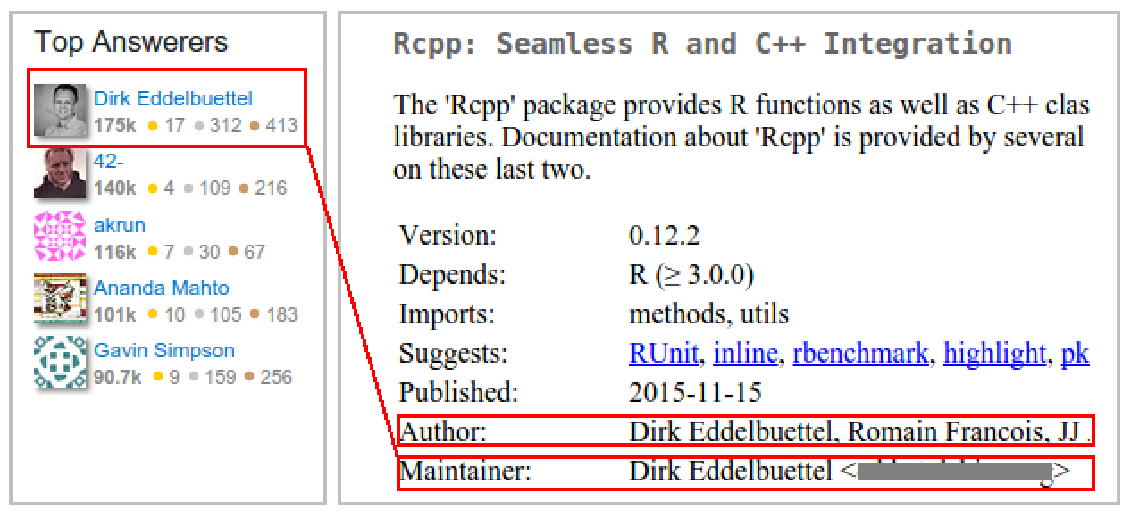
\includegraphics[width=0.7\columnwidth]{Figures/CCchannel}
			\caption{Example of how developers of the \emph{rcpp} package can be reached. On the left, Stack Overflow, and on the right, the webiste of \emph{rcpp}.}
			\label{fig:CCchannel}
		\end{figure}

		Finally, some channels are more suitable for certain \emph{type or format of questions}. 
		For example, R-help mailing list is a place for discussion, and Stack Overflow is a place for questions that have a clear answer.


	\subsubsection{Read the user manuals, channel rules and learn the basic concept of the technology used}

		Through the study, I noticed that most of the harsh responses from the community were give to users who did not read the posting guide or learned the basic concept for each technology (e.g., \textit{``An Introduction to R''}\footnote{\url{https://cran.r-project.org/doc/manuals/r-release/R-intro.pdf}})---users should demonstrate a minimum understanding and use of the programming language.
		The community expects that if someone wants to use a channel, they should learn about it in advance, and learn the basics of the technology that they are using.
		For instance, in the R-help's thread \textit{``Quantile''}\footnote{\url{http://goo.gl/Dc8gXw}} it is remarked the points of a guide that the user asking the question did not follow: \textit{``...Please read the Posting Guide. It asks that you not crosspost. If you post a followup to rhelp, then the reading of the Posting guide will tell you that much more in the way of detail about your setup was requested...''}.

		Depending on the channel, the amount of guide lines and posting guides available might differ. 
		Stack Overflow provides user manuals for each of the main features of the channel such as badges, questions\footnote{\url{http://stackoverflow.com/help/how-to-ask}}, answers\footnote{\url{http://stackoverflow.com/help/how-to-answer}}, flags, comments, and reputation system\footnote{\url{http://stackoverflow.com/help/whats-reputation}}.
		In contrast, the R-help mailing list only has the general instructions\footnote{\url{https://www.r-project.org/mail.html\#instructions}} and the posting guide user manual\footnote{\url{https://www.r-project.org/posting-guide.html}}, which make the R-help mailing list a more user friendly environment for new users in terms of what users have to read in advance.

		Moreover, depending on the technology, there are some \textit{community} user manuals that might be useful to read before participating in the channel.
		For instance, the post on Stack Overflow \textit{``How to make a great R reproducible example?''}\footnote{\url{http://stackoverflow.com/questions/5963269/how-to-make-a-great-r-reproducible-example}} provides tips and tricks for creating a reproducible example using the R language.
	 	Another example is the channel related user manual written by Hadley Wickham.
	 	It provides some tips for posting on the R-help mailing lists: \textit{``...Before putting all of your code in an email, consider putting it on \href{http://gist.github.com/}{[GitHub Gist app]}. It will give your code nice syntax highlighting, and you don't have to worry about anything getting mangled by the email system...''}

		Finally, there are technology manuals like \textit{``An Introduction to R''}), and the FAQ webpages that are available to the public---most of the time free of charge, from which any user can learn the basic of each technology.
		For instance, the R community provides a compendium of PDF documents for new users on different languages\footnote{The R Manuals are available at \url{https://cran.r-project.org/}}.
		While on Stack Overflow, supported technologies are provisioned with webpages and links to free and paid materials\footnote{Materials available at \url{http://stackoverflow.com/tags/r/info}}.
		Members are able to reference these materials when needed, e.g., \textit{``...You may want to acquaint yourself with the 'An Introduction to R' manual that came with your R installation to learn more about indexing.''}
		Figure~\ref{fig:RManuals} depicts the webpage on Stack Overflow with references to free and paid materials that can be reached using the info tab (on the left), and the R project website with free user manuals for the R language (on the right).

		\begin{figure} [!htb]
			\centering
			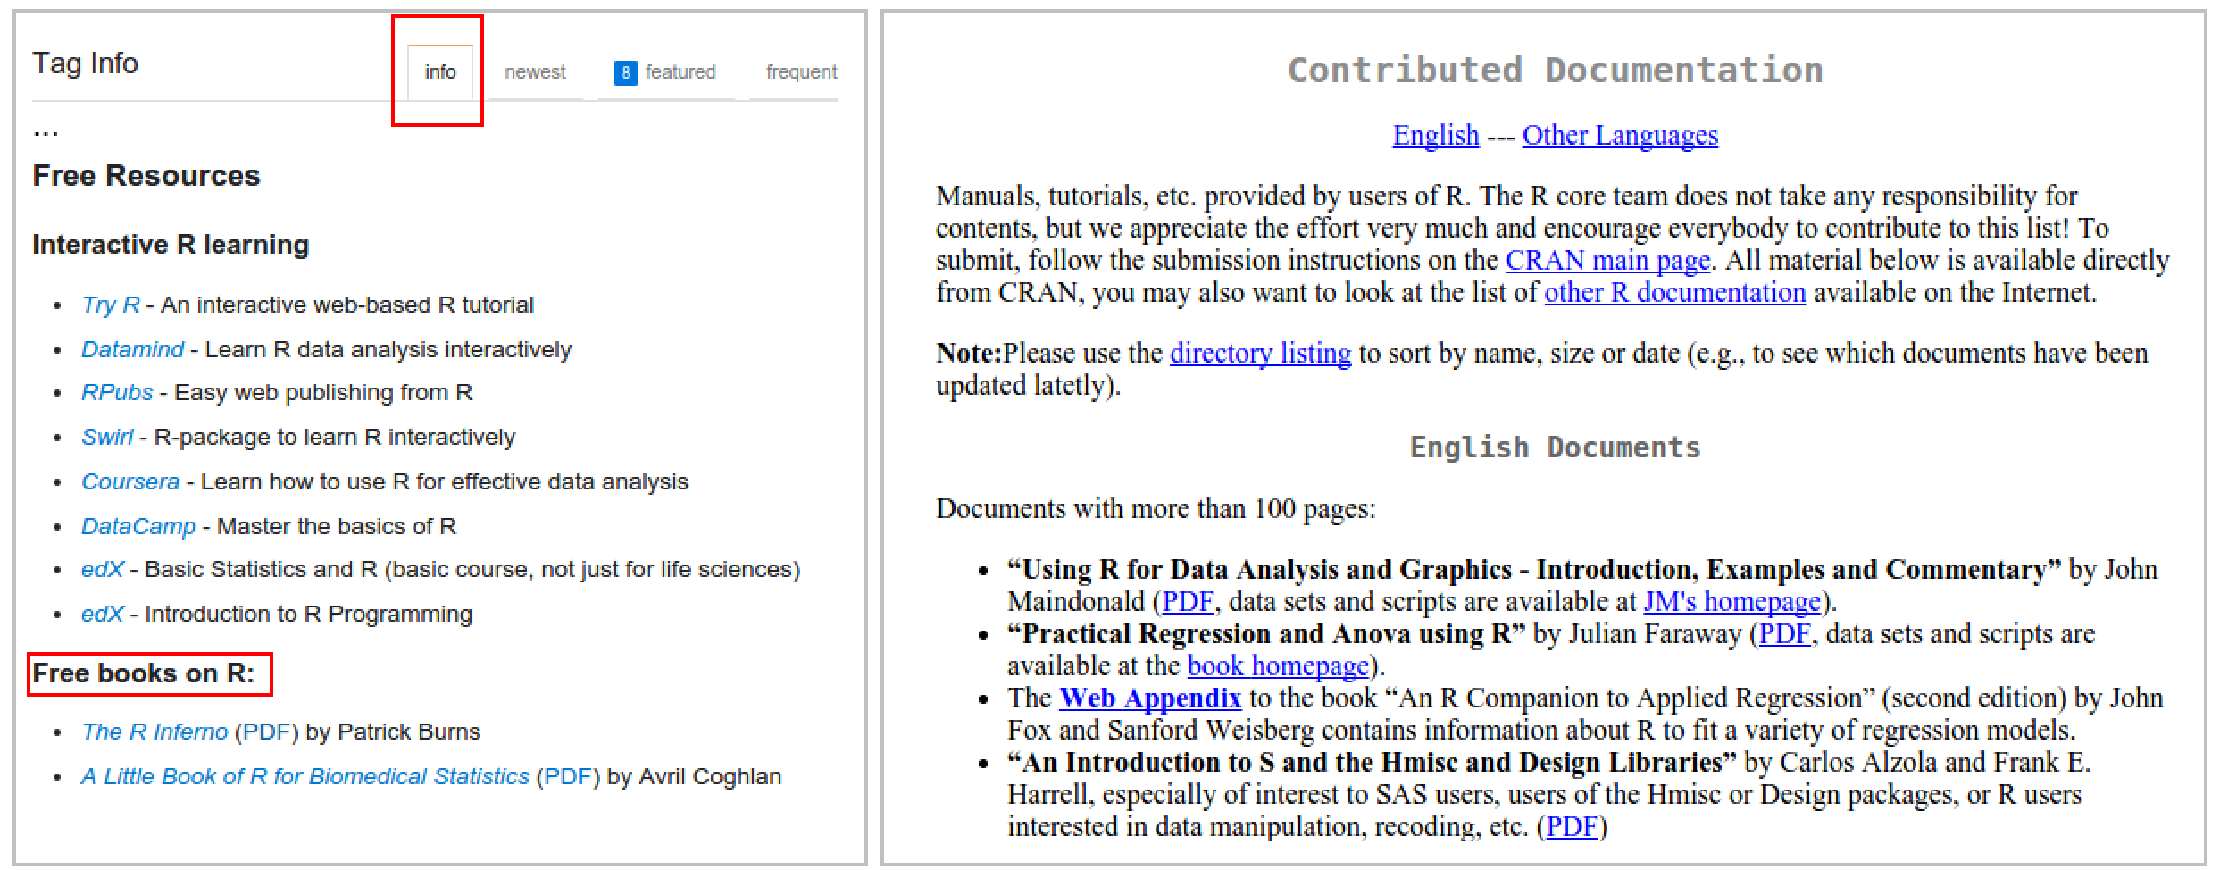
\includegraphics[width=1\columnwidth]{Figures/RManuals}
			\caption{Examples of free and paid manuals available through Stack Overflow and the technology community websites}
			\label{fig:RManuals}
		\end{figure}

	\subsubsection{Choose a channel according to the user experience}
		%Choose the less complex channel--- for newcomers

		Clearly, the variety of media channels can be overwhelming when having to choose one channel to post a question.
		Personal preferences (e.g., to use the most popular channel, or the one that answers question faster) are important elements when making a decision.
		It is always good to know the characteristics of the channels as a way to make a wise choice.
		For example, using Stack Overflow has many benefits such as low response time~\cite{Mamykina2011} and peer recognition~\cite{Singer2013}, but there are many user manuals that should be read prior participation, and a bad reputation in the channel might affect users in real life \cite{Singer2013}.
		U14 said that one of the biggest challenges of using Stack Overflow is learning the \emph{ethos} of the channel (see table \ref{table:surveySO})

		Sometimes communities have more than one channel that overlaps functionality with others.
		The R-help mailing list can be used for the same purpose as Stack Overflow, but it has a different audience as well as other benefits as demonstrated on this thesis.
		For instance, the R-help mailing list is less confronting (see table \ref{table:surveyML}-\textit{confrontation}); it can be used to learn rather than just get the answer (see table \ref{table:surveyML}-\textit{learning}, and \ref{table:surveySO}-\textit{To the point}); and it can be sometimes friendlier (see table \ref{table:surveySO}-\textit{Friendliness}).

	\subsubsection{Provide a Background to the Question}

        Sometimes, in spite of reading the documentation available, a user can fail to address the channel appropriately. 
        The community may feel that the question asked, the information provided or something else is not in compliance with the expectations and rules of the channel (e.g., read the posting guide, demonstrate minimum knowledge about the technology used).
		In such cases, one should describe the documentation read, the attempts made to answer the question on their own, and what they are actually trying to achieve.
		This would avoid answers like \textit{``read the manual''}, or \textit{``read the posting guide''}, as well as helping the participants to help.
		As an example, in the thread \textit{``lme4 GLMM''}\footnote{\url{https://goo.gl/Gbek3R}}, a user asked \textit{``I'm very sorry for my repeated question, which I asked 2 weeks ago, namely: I'm interested in possibly simple random-part specification in the call...''}.

\subsection{Recommendations For Using External Resources}

	When answering or asking questions, it is a common practice to provide links for sharing documentation, examples, source code, or other resources.
	As links point to online resources that might or not exist in the future, it is important to include the key points of the resource within the question or answer.
	For instance, when a question or answer contains information in an external file hosting service like Dropbox or Google Drive, the owner of the service account can break the link in any moment, leaving the message incomplete or impossible to reproduce, like the thread \textit{``Is it possible to create a 3d contour plot without continuous data in R?''}\footnote{\url{http://goo.gl/5nanFU}}.
	U33 suggested: \textit{``Questions should be self-contained as much as possible. Exceptions: recognizable links such as CRAN, R documentation, etc.''}.

	Based on our observations, I constructed a set of recommendations for links that are the exception of the rule:

	\begin{itemize}
		\item \emph{Well known websites}, that are expected to be maintained in the long term like Wikipedia, the official documentation in CRAN.
		For example, the Stack Overflow's thread \textit{``calculating convolution of multinomial distribution''}\footnote{\url{http://goo.gl/OAXoCl}} a user posted \textit{`I'm doing a simulation where I need to calculate a \href{https://en.wikipedia.org/wiki/Convolution_of_probability_distributions}{[Wikipedia convolution]} of \href{https://en.wikipedia.org/wiki/Multinomial_distribution}{[Wikipedia multinomial distributions]}...''}.

		\item Resources that support or \emph{expand the message}, but the important information is already explained in the message.
		For instance, the Stack Overflow's thread \textit{``How do I save all the draws from a MCMC posterior distribution to a file in R''}\footnote{\url{http://goo.gl/6YfShw}} clarifies \textit{``...You should be able to open a text connection using ?file \href{http://stat.ethz.ch/R-manual/R-devel/library/base/html/connections.html}{[more information]} with the open argument set to write...''}.

		\item The \emph{material relevant to the message is too big}, such as papers, or demonstrations.
		For instance, the R-help's thread \textit{``Using FUNCTION to create usable objects''}\footnote{\url{http://goo.gl/xF1j3R}} a user stated \textit{``I suspect you are trying to find your way into Circle 6 of 'The R Inferno' but haven't yet got in. \href{http://www.burns-stat.com/pages/Tutor/R\_inferno.pdf}{[R Inferno]}''}.
	\end{itemize}


\section{Discussion}
\label{cha:discussion}

	In this chapter, I discuss the findings presented in this thesis related with the analysis of the knowledge flow through Stack Overflow and the R-help mailing list in relation with the literature. 
	I also present the implication of the study and how it can be used for future research.

\subsection{Comparison of the Way Knowledge is Shared on Both Channel}

	Based on my findings, Stack Overflow is more suitable for questions with a clear answer, and the R-help mailing list is more suitable to discuss topics that are in and out of the software development domain.
	The study by Squire~\cite{Squire2015a} presents a similar difference between Stack Overflow and a mailing list of multiple projects through a different approach. 
	By studying communities that migrated development support towards Stack Overflow, Squire found that the main reason for communities coming back to the mailing list are topic restriction and the question's format expected on Stack Overflow.
	Squire and I suggest that communities of practice should evaluate what are the real benefits of each channel before moving to newer technologies.

	The comparison between channels presented in this thesis, as well as Vasilescu's work~\cite{Vasilescu2014c} about migration from Stack Overflow to the R-help mailing list, suggest that communities prefer to have access to a variety of answers (Stack Overflow), instead of single contextualized and discussed answers (the R-help mailing list). 
	To support this inference I presented two ways the community of the channel constructs knowledge: crowd and participatory. 
	The main benefit of using crowd knowledge construction is the existence of a pool of solutions, which combined with curation mechanisms, produces multiple ways to solve the same problem (diversity of solutions) in a clear solution that can be reused.

	Squire's study~\cite{Squire2015a} as well as my findings suggest that Stack Overflow might not be enough to fully support software developers.
	As it is suggested by the amount of active users on the R-help mailing list, a community might require a place to discuss topics that are in and out of the software development domain.
	Additionally, the fragmentation of topics within the Stack Exchange's Q\&A channels (each channel from Stack Exchange supports a small group of topics), the complex rules of their sites, and the gamification mechanism might be a difficult issue to handle for some users~\cite{Vasilescu2013}.
	However, more studies are necessary in order to confirm my inferences. 

	Finally, this study shows that the difference between media channels might be more complex than just the differences based on channels' features. 
	Every feature (e.g., gamification) might: affect the way in which community members work~\cite{Antin2011,Singer2013}, push away part of the community members~\cite{Vasilescu2013}, or change the way the knowledge is constructed.

\subsection{Message Categorization}

	In this thesis my colleague and I categorised the messages and the resources that flow through Stack Overflow and the R-help mailing list.
	In a previous study, Treude \textit{et al.}~\cite{Treude2011} categorized questions of different communities on Stack Overflow.
	The question categories \textbf{How-to}, \textbf{Bug/Error/Exception}, \textbf{Set-up}, \textbf{Decision help}, \textbf{Code reviewing}, and \textbf{Discrepancy} presented in this work, mirror the findings from Treude \textit{et al}. 
	The differences between my study and the study by Treude \textit{et al.} lie on the type of messages (i.e., questions, answers, updates, flags and comments) and community that my colleague and I analysed. 
	The question categorization presented in this work extends Treude \textit{et al.} findings by identifying a similar set of question categories over a different community and media channel (the R-help mailing list).

	%<<
%	Moreover, the message categorization proposed in this thesis was meant to be non-exclusive. 
%	The messages examples in chapter \ref{cha:findings} were primary classified in only one of the categories.
%	However, these messages might be also classified in other categories.
	%>>

	I believe that my categorization can help future studies to compare the knowledge of multiple channels by providing a common ground for comparison. 
	Furthermore, futures studies can extend our categories to include knowledge classification from other type of channels or domains. 
	Understanding the knowledge that flows through the channels might help to improve the tools that support developers. 
	Moreover, my knowledge categorization can be used to analyse in more detail the knowledge that flows through a channel. 
	For instance, it can be used to analyse unanswered questions~\cite{Asaduzzaman2013}, successful answers~\cite{Calefato2015}, or identify topic trends for each categorization type.

\subsection{Knowledge Construction}

	In this work, I present two ways to construct knowledge, the participatory and the crowd knowledge construction described in chapter \ref{cha:findings}.
	Tausczik \textit{et al}.~\cite{Tausczik2014} found the same collaborative knowledge construction over another knowledge domain and channel, the mathematics domain on Math Overflow (a Q\&A channel focused on solving mathematical problems).
	My findings extends what Tausczik \textit{et al}. found to other media channels and domains.

	The findings of this thesis can be used to identify how channels' features or community members might affect the construction of knowledge.
	For instance, I identified that gamification might affect collaboration between users. 
	Users prefer to create their own answer instead of collaborating with others.
	Additionally, it might be possible for indirect collaboration, like the one happening on the comments on Stack Overflow to improve discussion and participatory knowledge construction if there was a mechanism to provide points for this type of participation.
	However, more studies are required to extend my observation to other domains, communities, and channels.

	Moreover, through the survey I identified that there are certain benefits for keeping the history of the question available.
	As U26 said, there are some benefits to reading what a user thinks is not important for conceptualized questions, but which may lead to out of the frame thinking. 

	I believe that is important to understand how the knowledge is constructed on media channels, and how different mechanisms such as gamification or topic restriction can affect the knowledge construction~\cite{Li2015}.
	Through this understanding, researchers can gain insights of how to support future media channels, and user diversity~\cite{Vasilescu2014b}. 	

\subsection{GTMail}

	As previously mentioned in section \ref{sec:studyDesign}, I developed GTMail\footnote{Our open source JAVA tool is available online at \url{https://github.com/cagomezt/GTMail}}, a software tool used to pre-process the date from the R-help mailing list archives. 
	A few months later after creating my tool, and while my colleague and I were doing the analysis of the data, I noticed that Bettenburg has a similar tool based on his research\footnote{\url{https://github.com/nicbet/MailboxMiner}}.
	The main differences between my tool and Bettenburg's tool lays in the extra features added to deal with the particular issues presented in our data and the requirements of our study.
	Specifically, one of the requirements was downloading emails with coding issues from the URL left by the mailing list server after scrubbing the body, as well as dealing with standardizations issues (e.g., email addresses), and extraction of URLs resources. 
	All those changes can be added as extensions to Bettenburg's tool.

	Moreover, the extraction of URLs resources can be useful to analyse technology diffusion over media channels. 
	For instance, Squire \textit{et al}.~\cite{Squire2015} analysed URLs on different mailing list archives to identify the diffusion of tools such Pastebin and GitHub Gist (tool that support snippet code sharing, and syntax highlighting).

	One of the cleaning data processes that I never implemented in the GTMail tool was the elimination of source code from the body of the message. 
	As a consequence, this thesis relies on manual procedures to code the data as it was unnecessary to create the cleaning data step.
	However, according to Bacchelli \textit{et al}.~\cite{Bacchelli2012a}, the process of differentiating source code from users' messages might be necessary when analysing unstructured data from programmers (e.g., emails) using natural language processing techniques (e.g., Latent Dirichlet allocation or latent semantic analysis). 
	The approach of Bacchelli \textit{et al}.~\cite{Bacchelli2012a} could be a valuable extension to Bettenburg's tool.


\section{Threats to Validity and Limitations}
\label{cha:threats}

    This chapter outlines the threats to the validity of this study. As we had multiple researchers coding the data, and found using a case study methodology to be a challenging task, multiple limitations surfaced.

%\subsection*{Construct Validity}
%
%	%<<
%	According to Runeson~\cite{Runeson2012}, construct validity refers to the extent in which the operational measurements that are being studied, represent what the researcher has in mind and what is being investigated according to the research questions.
%	In this thesis, the GTMail tool was tested manually, and through out the study of the R-help mailing list data (see Appendix \ref{cha:appendicesD}).
%	All tests that I performed were not exhaustive, or formal.
%	In addition, the GTMail tool was not compared against other tools that accomplish the same objective (e.g., MailingListStats, and REmail), neither tested to be resilient to all the possible errors that might exist in the data.
%	This issue might represent a threat to validity of the GTMail tool.
%	%>>

\subsection{Internal Validity}

%	It is important to clarify that given the exploratory nature of the study, the evidence found in this work is not statistically significant
	Internal validity refers to the amount of bias within a study~\cite{Creswell2009}. 
	In an exploratory case study, the researchers' actions and biases affect the finished work in each step,  
	such as during the selection and analysis of data. 

	In this study, two researchers with a similar background---both computer scientists from the same country, with English as their second language---	worked together to code the data. 
	The open coding technique used in this work involved the analysis of large collections of messages based on the researchers' observations. 
	Our background might have biased how we coded the data, as well as our understanding of the context of the study. 
	Additionally, our results may have been influenced by the method we used to select data for analysis (as explained in section \ref{subsec:preparation}) or the pre-processing of the information that we did before loading the data to the database (as explained in section \ref{sec:dap}), which might be influence the reconstruction of threads for the R-help mailing list. 
	Moreover, there may have been bias in the mapping of message types between Stack Overflow and the R-help mailing. As the R-help mailing list contains unstructured data, our understanding of that data and the observations we made played a big role in the mapping exercise. 

	%<<
	In terms of the techniques applied during the study, I used Cohen Kappa coefficient on categories that were not mutually exclusive. 
	The purpose of calculating the coefficient were solely to trigger discussion between coders. 
	However, it might introduce bias to the study as a consequence of Cohen Kappa's limitations---it should be applied over mutually exclusive categories.
	%>>

	As consequence of our exploratory case study methodology and the parallel execution of \textit{phase 1} and \textit{2}, some of the survey results were not aligned with our findings. 
	Moreover, the survey recruitment methods listed in chapter \ref{cha:discussion} might have biased the population. 
	For instance, when we announced the survey through Stack Overflow, moderators removed our message a few minutes after we posted; for this reason, it is possible that we did not reach enough of the Stack Overflow population.
	The number of responses to the survey and the high variability of the answers might also contribute to the analysis bias---given that we could not obtain enough participants, we had to support users' opinions with just a few responses.  
	The survey questions were created solely by the author of this thesis, and while we tried to conduct pilot studies, no one else had a thorough enough understanding of the research. 
	After the survey data was collected, the author was the only researcher that analysed the information.
	Finally, as a consequence of running the survey phase in parallel with the data analysis some of the survey responses are not aligned with the results of this thesis.

	In terms of the tool presented in this thesis, our biggest limitation was identifying the existence of Bettenburg tool while we were already conducting the analysis.
	Indeed there are two different approaches that solve the same problem and that are based on the same process of data cleaning.
	However, some of the GTMail tool features can be applied to Bettenburg as an extension of his work.

	Moreover, the GTMail tool was tested manually, and through out the study of the R-help mailing list data.
	All tests that I performed were not exhaustive, or formal.
	In addition, the GTMail tool was not compared against other tools that accomplish the same objective (e.g., MailingListStats, and REmail), neither tested to be resilient to all the possible errors that might exist in the data.
	This issue might represent a threat to validity of the GTMail tool.

	%Moreover, I did not measure how accurate was the GTMail tool to recreate the data from the R-help mailing list, neither compare the tool against other tools. 
\subsection{External Validity}

	External validity is concerned with the extent to which the findings from this work can be generalized~\cite{Runeson2012, Calder1982}. 
	As a case study, it cannot be assumed that these cases can be generalizable until further evaluations have been conducted~\cite{Yin2009}.
	%<<
	The best example of the previous statement is that this thesis studied developers from the R community, which are not typical programmers.
	I consider R language users as \textit{casual developers} due to their limited (or non-existent) programming experience (e.g., biologists or statisticians).
	The R programming language is used to solve statistical problems, but it does not create any software product or tool at the end of the programming process---the final product is a script that process a specific data.
	As a consequence, this study might not represent the knowledge that a typical software developer community shares.
	%>>

	According to Yin~\cite{Yin2009}, \textit{``a case study (as with experiments) rely on analytic generalization. In analytical generalization, the investigator is striving to generalize a particular set of results to some broader theory''}. 
	For this reason, findings in this research should be tested in other communities and with other channels to see if our findings would apply to these other contexts.
	There are some of my findings that are prove to be true over other knowledge domains, communities, or media channels. 
	For instance, there are other studies that support some of our findings in other communities, such as Tausczik \textit{et al.}~\cite{Tausczik2014} (i.e., knowledge construction) and Treude \textit{et al.}~\cite{Treude2011} (i.e., question categorization).

\subsection{Standards of Rigour}
	This work incorporated a number of approaches to minimize the threats to validity mentioned above and to establish rigour~\cite{Runeson2012,Yin2009}.	
	These approaches included triangulating multiple sources of data (i.e., survey, documentation, and messages from both media channels), randomly selecting data, and using multiple researchers to code the data. 
	As a result, we were able to identify and report discrepancies and contradictions.

	This study was conducted over a one-year period in which we were heavily immersed in the information within the channel, such as messages and official community documentation. This allowed us to gain a good understanding of the context and the community. 
	When we began to code the data, I told my colleague to code by ``what she observed'', avoiding any previous knowledge she had related to the topic (if any). 
	The description of what we had to code was intentionally vague in order to minimize researcher bias.
	As was expected, our categorization did not always align, however, 
	we came to agree on our interpretation of the data before starting the next coding session. 
	As mentioned before, we used an inter-rater agreement coefficient (i.e., Cohen Kappa) to measure our mutual understanding and to promote discussion.

	In terms of the data selection process, we minimized the threats by randomly selecting the data to analyse (see chapter \ref{cha:methodology}).
	This guaranteed that the information selected had the same probability of being chosen for the study.

	In summary, even with all the countermeasures that we applied to minimize bias, our findings are limited by our experience in the qualitative research environment and our vision of the world.   


\section{Future Work}
\label{cha:future-work}

	In this thesis, I was motivated to investigate the way programmers use media channels to share \textit{knowledge} within a particular software development community. 
	I decided to study two channels within the R community: the R-help mailing list and Stack Overflow.
	During the development of this thesis, I identified several dimensions related to knowledge: a classification of types of knowledge, categories and properties; a set of recommendations for the usage of multiple media channels; and an understanding of knowledge construction. 
	The following subsections outline areas for future work based on our findings.

	% Generalization of these findings. Explore other communities both with mailing list and QA website.
	\paragraph{Is the categorization of knowledge different in other software development communities?}

	I presented a model for analysing knowledge based on the comparison of two Q\&A channels. 
	While my study was limited to the R community and two of its channels (the R-help mailing list and Stack Overflow), 
	other developer communities (e.g., Firefox, Linux, or Android) also use Q\&A channels.
	I believe that the type of knowledge (i.e., categories and properties) might be very similar among these other communities, but found in different channels.
	To address this question, our model can be applied to other similar communities of practice.

	% Verify if the topics are the same 
	\paragraph{Are the topics of discussion the same for the R-help mailing list and Stack Overflow?}

	I studied these two channels to understand the types of knowledge they shared, which I found to be very similar. 
	However, I did not study the topics of discussion they contained.
	I am interested in identifying if both channels discussed the same topics with the purpose of assisting users when posting questions to the correct channel. 
	To address this question, there are automatic techniques that can be applied. For instance, Latent Dirichlet Allocation (LDA)\footnote{\url{https://en.wikipedia.org/wiki/Latent_Dirichlet_allocation}} is a natural language processing technique that is used to analyse large bodies of text.

	% Changes over mailing list
	\paragraph{What should be the next evolutionary step for the R-help mailing list?}

	My study identified that the R-help mailing list brings the discussion benefit to the R community. 
	I feel that this shows its importance within the R community.
	Survey participants provided a list of things that can be implemented to improve the experience for R-help's users.
	I am interested in understanding the next logical step of evolution for the R-help mailing list to continue supporting its extensive user base.
	To address this question, functional and non-functional requirements need to be evaluated, along with the execution of user studies (e.g., surveys and interviews) to address specific usage concerns.


\section{Concluding Remarks}
\label{cha:conclusion}

	This thesis explores the knowledge that flows through Stack Overflow and the R-help mailing list within the R community.
	In my approach, we performed a systematic comparison of both media channels and performed open coding to understand and classify knowledge.
	In order to conduct a fair comparison, I collected raw data from both channels (i.e., XML and MBOX files), transformed this data to a common format (i.e., analysis of the messages to map questions, answers, and other elements), and uploaded the information into databases to facilitate queries and other study-related activities.

	Two researchers performed iterative open coding and attended regular meetings to compare results.
	After the analysis of more than 500 threads, we identified five types of messages (i.e., question, answer, comment, update, and flag) and more than 35 categories (along with their properties), including how-to question, tutorial answer, announcement update, not-an-answer flag, and clarifications comment (for the complete list, refer to chapter \ref{cha:findings-types}).

	Additionally, my colleague and I identified two mechanisms for the construction of knowledge: participatory, in which answers are created with the collaboration of various users; and crowd-based, which is non-collaborative and where solutions are posted without any acknowledgement to previous answers.
	We also analysed links and how these contribute to the construction of knowledge, such as by referencing source code, projects, and other posts related to a particular question.

	Furthermore, my colleague and I identified user behaviours based on their comments and noted certain usage characteristics in both channels (i.e., analysing equivalent questions in the same subject, by the same user posted in both channels), including solving their own question and providing the answer, and cross-posting.

	Finally, I conducted a survey that collected 26 answers from R users in order to bring further insights on the findings of this thesis. 
	My survey provided us with a list (based on the participants' opinions) of the pros and cons of using both channels that I incorporated into the set of recommendations for using multiple channels, and resources.

	In this work, I pose that understanding the interplay between channels should be the next step to gain further insights into software development practices.
	To that end, I provided a contrast of the way knowledge is shared on Stack Overflow and the R-help mailing list, as well as an extensible categorization of Q\&A channel messages that is meant to be used to compare and analyse knowledge in media channels.
	Additionally, I included a set of recommendations for using multiple media channels and external resources, a tool to pre-process MBOX format mailing list archives, and R community insights based on the analysis of the knowledge categorization and observations.
	I hope that my research will be useful to other researchers interested in how developers share knowledge.


\bibliographystyle{abbrv}
\bibliography{references}

\end{document}
